% Created 2011-09-12 Mon 13:52
\documentclass[captions=tableheading]{scrbook}



\subtitle{Second Edition}

\usepackage{lmodern}
\renewcommand{\sfdefault}{lmss}
\renewcommand{\ttdefault}{lmtt}

% needed packages
\usepackage{amsmath}
\usepackage{amssymb}
\usepackage{amsthm}
\usepackage[english]{babel}
\usepackage{epsfig}
\usepackage{fancyvrb}
\usepackage{fixltx2e}
\usepackage{float}
%\usepackage{floatflt}
\usepackage[T1]{fontenc}
\usepackage{footnote}
%\usepackage{graphics}
\usepackage{graphicx}
\usepackage[utf8]{inputenc}
\usepackage{latexsym}
\usepackage{longtable}
\usepackage{makeidx}
\usepackage{marvosym}
\usepackage{multicol}
%\usepackage{pslatex}
%\usepackage{showidx}
\usepackage{soul}
\usepackage{srcltx}
\usepackage{stmaryrd}
\usepackage{subfig}
\usepackage{textcomp}
%\usepackage{theorem}
\usepackage[subfigure]{tocloft}
\usepackage{txfonts}
\usepackage{upgreek}
\usepackage{url}
\usepackage{varioref}
\usepackage{verbatim}
%\usepackage{wasysym}
\usepackage{wrapfig}


% Page setup
\usepackage[paperwidth=7.44in,paperheight=9.69in]{geometry}
\geometry{verbose,tmargin=1in,bmargin=1in,lmargin=1in,rmargin=1in}
\pagestyle{headings}
\setcounter{secnumdepth}{2}
\setcounter{tocdepth}{1}

\makeindex

% PDF settings
\usepackage[hyperref,x11names]{xcolor}
\usepackage[	unicode=true, 
		bookmarks=true, 
		bookmarksnumbered=true, 
		bookmarksopen=true, 
		bookmarksopenlevel=0, 
		breaklinks=true,
		pdfborder={0 0 0},
		backref=page,
		colorlinks=true]{hyperref}
\hypersetup{pdftitle={Introduction to Probability and Statistics Using R},
 		pdfauthor={G. Jay Kerns}, 
		linkcolor=Firebrick4, 
		citecolor=black, 
		urlcolor=SteelBlue4}

% Listings setup
\usepackage{color}
\usepackage{listings}
\lstset{basicstyle={\ttfamily},
	language=R,
	breaklines=true,
	breakatwhitespace=true,
	keywordstyle={\ttfamily},
	numberstyle = {\ttfamily},
	morestring=[b]"
}




%%%%%%%%%%%%%%%%%%%%%%%%%%%%%% LyX specific LaTeX commands.
\providecommand{\LyX}{L\kern-.1667em\lower.25em\hbox{Y}\kern-.125emX\@}
\newcommand{\noun}[1]{\textsc{#1}}
%% Because html converters don't know tabularnewline
\providecommand{\tabularnewline}{\\}

% special logos
\providecommand{\IPSUR}
{\textsc{I\kern 0ex\lower-0.3ex\hbox{\small P}\kern -0.5ex\lower0.4ex\hbox{\footnotesize S}\kern -0.25exU}\kern -0.1ex\lower 0.15ex\hbox{\textsf{\large R}}\@}

%  user defined commands
% special operators

\renewcommand{\vec}[1]{\mbox{\boldmath$#1$}}

\makeatletter

%%%%%%%%%%%%%%%%%%%%%%%%%%%%%% Textclass specific LaTeX commands.

\numberwithin{equation}{section}
\numberwithin{figure}{section}

\theoremstyle{plain}
  \newtheorem{thm}{Theorem}[chapter]
  \newtheorem{fact}[thm]{Fact}
  \newtheorem{ax}[thm]{Axiom}
  \newtheorem{prop}[thm]{Proposition}
  \newtheorem{cor}[thm]{Corollary}
  \newtheorem{assumption}[thm]{Assumption}

\theoremstyle{definition}
  \newtheorem{defn}[thm]{Definition}
  \newtheorem{example}[thm]{Example}
  \newtheorem{xca}{Exercise}[chapter]

\theoremstyle{remark}
  \newtheorem{note}[thm]{Note}
  \newtheorem{rem}[thm]{Remark}
  \newtheorem*{note*}{Note}

\setlength{\cftfignumwidth}{1.5cm}

\@ifundefined{showcaptionsetup}{}{%
 \PassOptionsToPackage{caption=false}{subfig}}
\usepackage{subfig}
\AtBeginDocument{
  \def\labelitemii{\(\circ\)}
}

\makeatother


\newenvironment{exampletoo}{\begin{example}}{\end{example}}


\providecommand{\alert}[1]{\textbf{#1}}

\title{\fontsize{30}{35}\selectfont Introduction to Probability and Statistics Using \textsf{R}}
\author{\fontsize{24}{28}\selectfont G. Jay Kerns}
\date{\fontsize{24}{28}\selectfont \noun{Second Edition}}

\begin{document}

\maketitle

% Org-mode is exporting headings to 3 levels.


\pagenumbering{roman}
\setcounter{page}{2}

\noindent \IPSUR: Introduction to Probability and Statistics Using \textsf{R}

\noindent Copyright \textcopyright~2011 G.~Jay Kerns
\noindent ISBN: 978-0-557-24979-4
\medskip{}


\noindent Permission is granted to copy, distribute and/or modify
this document under the terms of the GNU Free Documentation License,
Version 1.3 or any later version published by the Free Software Foundation; with no Invariant Sections, no Front-Cover Texts, and no Back-Cover Texts. A copy of the license is included in the section entitled ``GNU Free Documentation License''.

\vspace{0.25in}
\noindent Date: \today
\noindent \vfill{}

\cleardoublepage
\phantomsection
\pdfbookmark[1]{Contents}{table}

\tableofcontents{}



\chapter*{Preface}

This book was expanded from lecture materials I use in a one semester upper-division undergraduate course entitled \emph{Probability and Statistics} at Youngstown State University. Those lecture materials, in turn, were based on notes that I transcribed as a graduate student at Bowling Green State University. The course for which the materials were written is 50-50 Probability and Statistics, and the attendees include mathematics, engineering, and computer science majors (among others). The catalog prerequisites for the course are a full year of calculus.

The book can be subdivided into three basic parts. The first part includes the introductions and elementary \emph{descriptive statistics}; I want the students to be knee-deep in data right out of the gate. The second part is the study of \emph{probability}, which begins at the basics of sets and the equally likely model, journeys past discrete/continuous  random variables, and continues through to multivariate distributions. The chapter on sampling distributions paves the way to the third part, which is \emph{inferential statistics}. This last part includes point and interval estimation, hypothesis testing, and finishes with introductions to selected topics in applied statistics.

I usually only have time in one semester to cover a small subset of this book. I cover the material in Chapter 2 in a class period that is supplemented by a take-home assignment for the students. I spend a lot of time on Data Description, Probability, Discrete, and Continuous Distributions. I mention selected facts from Multivariate Distributions in passing, and discuss the meaty parts of Sampling Distributions before moving right along to Estimation (which is another chapter I dwell on considerably). Hypothesis Testing goes faster after all of the previous work, and by that time the end of the semester is in sight. I normally choose one or two final chapters (sometimes three) from the remaining to survey, and regret at the end that I did not have the chance to cover more.

In an attempt to be correct I have included material in this book which I would normally not mention during the course of a standard lecture. For instance, I normally do not highlight the intricacies of measure theory or integrability conditions when speaking to the class. Moreover, I often stray from the matrix approach to multiple linear regression because many of my students have not yet been formally trained in linear algebra. That being said, it is important to me for the students to hold something in their hands which acknowledges the world of mathematics and statistics beyond the classroom, and which may be useful to them for many semesters to come. It also mirrors my own experience as a student.

The vision for this document is a more or less self contained, essentially complete, correct, introductory textbook. There should be plenty of exercises for the student, with full solutions for some, and no solutions for others (so that the instructor may assign them for grading). By \texttt{Sweave}'s dynamic nature it is possible to write randomly generated exercises and I had planned to implement this idea already throughout the book. Alas, there are only 24 hours in a day. Look for more in future editions.

Seasoned readers will be able to detect my origins: \emph{Probability and Statistical Inference} by Hogg and Tanis \cite{Hogg2006}, \emph{Statistical Inference} by Casella and Berger \cite{Casella2002}, and \emph{Theory of Point Estimation} and \emph{Testing Statistical Hypotheses} by Lehmann \cite{Lehmann1998,Lehmann1986}. I highly recommend each of those books to every reader of this one. Some \textsf{R} books with ``introductory'' in the title that I recommend are \emph{Introductory Statistics with R} 
by Dalgaard \cite{Dalgaard2008} and \emph{Using R for Introductory Statistics} by Verzani \cite{Verzani2005}. Surely there are many, many other good introductory books about \textsf{R}, but frankly, I have tried to steer clear of them for the past year or so to avoid any undue influence on my own writing.

I would like to make special mention of two other books: \emph{Introduction to Statistical Thought} by Michael Lavine \cite{Lavine2009} and \emph{Introduction to Probability} by Grinstead and Snell \cite{Grinstead1997}. Both of these books are \emph{free} and are what ultimately convinced me to release \IPSUR under a free license, too.

Please bear in mind that the title of this book is ``Introduction to Probability and Statistics Using \textsf{R}'', and not ``Introduction to \textsf{R} Using Probability and Statistics'', nor even ``Introduction to Probability and Statistics and \textsf{R} Using Words''. The people at the party are Probability and Statistics; the handshake is \textsf{R}. There are several important topics about \textsf{R} which some individuals will feel are underdeveloped, glossed over, or wantonly omitted. Some will feel the same way about the probabilistic and/or statistical content. Still others will just want to learn \textsf{R} and skip all of the mathematics.

Despite any misgivings: here it is, warts and all. I humbly invite said individuals to take this book, with the GNU Free Documentation License (GNU-FDL) in hand, and make it better. In that spirit there are at least a few ways in my view in which this book could be improved.

\begin{description}
\item[Better data.] The data analyzed in this book are almost entirely from the \texttt{datasets} package in base \textsf{R}, and here is why:
\begin{itemize}
\item I made a conscious effort to minimize dependence on contributed packages,
\item The data are instantly available, already in the correct format, so we need not take time to manage them, and
\item The data are \emph{real}.
\end{itemize}
\end{description}

I made no attempt to choose data sets that would be interesting to the students; rather, data were chosen for their potential to convey a statistical point. Many of the data sets are decades old or more (for instance, the data used to introduce simple linear regression are the speeds and stopping distances of cars in the 1920's).

In a perfect world with infinite time I would research and contribute recent, \emph{real} data in a context crafted to engage the students in \emph{every} example. One day I hope to stumble over said time. In the meantime, I will add new data sets incrementally as time permits.

\begin{description}
\item[More proofs.] I would like to include more proofs for the sake of completeness (I understand that some people would not consider more proofs to be improvement). Many proofs have been skipped entirely, and I am not aware of any rhyme or reason to the current omissions. I will add more when I get a chance.
\item[More and better\~{}graphics.] I have not used the \texttt{ggplot2} package \cite{Wickam2009} because I do not know how to use it yet. It is on my to-do list.
\item[More and better exercises.] There are only a few exercises in the first edition simply because I have not had time to write more. I have toyed with the \texttt{exams} package \cite{exams} and I believe that it is a right way to move forward. As I learn more about what the package can do I would like to incorporate it into later editions of this book.
\end{description}


\section*{About This Document}

\IPSUR contains many interrelated parts: the \emph{Document}, the \emph{Program}, the \emph{Package}, and the \emph{Ancillaries}. In short, the \emph{Document} is what you are reading right now. The \emph{Program} provides an efficient means to modify the Document. The \emph{Package} is an \textsf{R} package that houses the Program and the Document. Finally, the \emph{Ancillaries} are extra materials that reside in the Package and were produced by the Program to supplement use of the Document. We briefly describe each of them in turn.

\subsection*{The Document}

The \emph{Document} is that which you are reading right now -- \IPSUR's \emph{raison d'\^etre}. There are transparent copies (nonproprietary text files) and opaque copies (everything else). See the GNU-FDL in Appendix \ref{cha:GNU-Free-Documentation} for more precise language and details.


\begin{description}
\item[IPSUR.tex] is a transparent copy of the Document to be typeset with a \LaTeX{} distribution such as Mik\TeX{} or \TeX{} Live. Any reader is free to modify the Document and release the modified version in accordance with the provisions of the GNU-FDL. Note that this file cannot be used to generate a randomized copy of the Document. Indeed, in its released form it is only capable of typesetting the exact version of \IPSUR which you are currently reading. Furthermore, the \texttt{.tex} file is unable to generate any of the ancillary materials.
\item[IPSUR-xxx.eps, IPSUR-xxx.pdf] are the image files for every graph in the Document. These are needed when typesetting with \LaTeX{}.
\item[IPSUR.pdf] is an opaque copy of the Document. This is the file that instructors would likely want to distribute to students.
\item[IPSUR.dvi] is another opaque copy of the Document in a different file format.
\end{description}

\subsection*{The Program}

The \emph{Program} includes \texttt{IPSUR.lyx} and its nephew \texttt{IPSUR.Rnw}; the purpose of each is to give individuals a way to quickly customize the Document for their particular purpose(s).


\begin{description}
\item[IPSUR.lyx] is the source \LyX{} file for the Program, released under the GNU General Public License (GNU GPL) Version 3. This file is opened, modified, and compiled with \LyX{}, a sophisticated open-source document processor, and may be used (together with \texttt{Sweave}) to generate a randomized, modified copy of the Document with brand new data sets for some of the exercises and the solution manuals (in the Second Edition). Additionally, \LyX{} can easily activate/deactivate entire blocks of the document, /e.g./\~{}the \textsf{proofs} of the theorems, the student \textsf{solutions} to the exercises, or the instructor \textsf{answers} to the problems, so that the new author may choose which sections (s)he would like to include in the final Document (again, Second Edition). The \texttt{IPSUR.lyx} file is all that a person needs (in addition to a properly configured system -- see Appendix \ref{cha:Instructions-for-Instructors}) to generate/compile/export to all of the other formats described above and below, which includes the ancillary materials \texttt{IPSUR.Rdata} and \texttt{IPSUR.R}.
\item[IPSUR.Rnw] is another form of the source code for the Program, also released under the GNU GPL Version 3. It was produced by exporting \texttt{IPSUR.lyx} into\textsf{ R}/Sweave format (\texttt{.Rnw}). This file may be processed with Sweave to generate a randomized copy of \texttt{IPSUR.tex} -- a transparent copy of the Document -- together with the ancillary materials \texttt{IPSUR.Rdata} and \texttt{IPSUR.R}. Please note, however, that \texttt{IPSUR.Rnw} is just a simple text file which does not support many of the extra features that \LyX{} offers such as WYSIWYM editing, instantly (de)activating branches of the manuscript, and more.
\end{description}



\subsection*{The Package}

There is a contributed package on \texttt{CRAN}, called \texttt{IPSUR}. The package affords many advantages, one being that it houses the  Document in an easy-to-access medium. Indeed, a student can have the Document at his/her fingertips with only three commands:



Another advantage goes hand in hand with the Program's license; since \IPSUR is free, the source code must be freely available to anyone that wants it. A package hosted on \texttt{CRAN} allows the author to obey the license by default.

A much more important advantage is that the excellent facilities at \textsf{R}-Forge are building and checking the package daily against patched and development versions of the absolute latest pre-release of \textsf{R}. If any problems surface then I will know about it within 24 hours.

And finally, suppose there is some sort of problem. The package structure makes it \emph{incredibly} easy for me to distribute bug-fixes and corrected typographical errors. As an author I can make my corrections, upload them to the repository at \textsf{R}-Forge, and they will be reflected \emph{worldwide} within hours. We aren't in Kansas anymore, Toto.

\subsection*{Ancillary Materials}

These are extra materials that accompany \IPSUR. They reside in the \texttt{/etc} subdirectory of the package source. 

\begin{description}
\item[IPSUR.RData] is a saved image of the \textsf{R} workspace at the completion of the Sweave processing of \IPSUR. It can be loaded into memory with \textsf{File} \(\triangleright\) \textsf{Load Workspace} or with the command \texttt{load("/path/to/IPSUR.Rdata")}. Either method will make every single object in the file immediately available and in memory. In particular, the data BLANK from Exercise BLANK in Chapter BLANK on page BLANK will be loaded. Type BLANK at the command line (after loading \texttt{IPSUR.RData}) to see for yourself.
\item[IPSUR.R] is the exported \textsf{R} code from \texttt{IPSUR.Rnw}. With this script, literally every \textsf{R} command from the entirety of \IPSUR can be resubmitted at the command line.
\end{description}

\section*{Notation}

We use the notation \texttt{x} or \texttt{stem.leaf} notation to denote objects, functions, \emph{etc}.. The sequence ``\textsf{Statistics} \textsf{\(\triangleright\)} \textsf{Summaries} \textsf{\(\triangleright\)} \textsf{Active Dataset}'' means to click the \textsf{Statistics} menu item, next click the \textsf{Summaries} submenu item, and finally click \textsf{Active Dataset}.

\section*{Acknowledgements}

This book would not have been possible without the firm mathematical and statistical foundation provided by the professors at Bowling Green State University, including Drs. G\'\{a\}bor Sz\'\{e\}kely, Craig Zirbel, Arjun K. Gupta, Hanfeng Chen, Truc Nguyen, and James Albert. I would also like to thank Drs.\~{}Neal Carothers and Kit Chan. 

I would also like to thank my colleagues at Youngstown State University for their support. In particular, I would like to thank Dr. G. Andy Chang for showing me what it means to be a statistician.

I would like to thank Richard Heiberger for his insightful comments and improvements to several points and displays in the manuscript. 

Finally, and most importantly, I would like to thank my wife for her patience and understanding while I worked hours, days, months, and years on a \emph{free book}. Looking back, I can't believe I ever got away with it.

\vfill{}
\cleardoublepage
\phantomsection
\addcontentsline{toc}{chapter}{List of Figures}
\listoffigures

\vfill{}
\cleardoublepage
\phantomsection
\addcontentsline{toc}{chapter}{List of Tables}
\listoftables



\chapter{An Introduction to Probability and Statistics}
\label{sec-1}

\pagenumbering{arabic} 

\noindent This chapter has proved to be the hardest to write, by far. The trouble is that there is so much to say -- and so many people have already said it so much better than I could. When I get something I like I will release it here.

In the meantime, there is a lot of information already available to a person with an Internet connection. I recommend to start at Wikipedia, which is not a flawless resource but it has the main ideas with links to reputable sources.

In my lectures I usually tell stories about Fisher, Galton, Gauss, Laplace, Quetelet, and the Chevalier de Mere.
\section{Probability}
\label{sec-1-1}


The common folklore is that probability has been around for millennia but did not gain the attention of mathematicians until approximately 1654 when the Chevalier de Mere had a question regarding the fair division of a game's payoff to the two players, if the game had to end prematurely.
\section{Statistics}
\label{sec-1-2}


Statistics concerns data; their collection, analysis, and interpretation. In this book we distinguish between two types of statistics: descriptive and inferential. 

Descriptive statistics concerns the summarization of data. We have a data set and we would like to describe the data set in multiple ways. Usually this entails calculating numbers from the data, called descriptive measures, such as percentages, sums, averages, and so forth.

Inferential statistics does more. There is an inference associated with the data set, a conclusion drawn about the population from which the data originated.

I would like to mention that there are two schools of thought of statistics: frequentist and bayesian. The difference between the schools is related to how the two groups interpret the underlying probability (see Section \ref{sec:Interpreting-Probabilities}). The frequentist school gained a lot of ground among statisticians due in large part to the work of Fisher, Neyman, and Pearson in the early twentieth century. That dominance lasted until inexpensive computing power became widely available; nowadays the bayesian school is garnering more attention and at an increasing rate.

This book is devoted mostly to the frequentist viewpoint because that is how I was trained, with the conspicuous exception of Sections \ref{sec:Bayes'-Rule} and \ref{sec:Conditional-Distributions}. I plan to add more bayesian material in later editions of this book.

\newpage{}
\section{Exercises}
\label{sec-1-3}

\setcounter{thm}{0}
\chapter{Data Description}
\label{sec-2}

\label{cha:Describing-Data-Distributions}

\noindent In this chapter we introduce the different types of data that a statistician is likely to encounter, and in each subsection we give some examples of how to display the data of that particular type. Once we see how to display data distributions, we next introduce the basic properties of data distributions. We qualitatively explore several data sets. Once that we have intuitive properties of data sets, we next discuss how we may numerically measure and describe those properties with descriptive statistics.

\paragraph*{What do I want them to know?}

\begin{itemize}
\item different data types, such as quantitative versus qualitative, nominal versus ordinal, and discrete versus continuous
\item basic graphical displays for assorted data types, and some of their (dis)advantages
\item fundamental properties of data distributions, including center, spread, shape, and crazy observations
\item methods to describe data (visually/numerically) with respect to the properties, and how the methods differ depending on the data type
\item all of the above in the context of grouped data, and in particular, the concept of a factor
\end{itemize}
\section{Types of Data}
\label{sec-2-1}

\label{sec:Types-of-Data}

Loosely speaking, a datum is any piece of collected information, and a data set is a collection of data related to each other in some way. We will categorize data into five types and describe each in turn:

\begin{description}
\item[Quantitative] data associated with a measurement of some quantity on an observational unit,
\item[Qualitative] data associated with some quality or property of an observational unit,
\item[Logical] data which represent true or false and play an important role later,
\item[Missing] data which should be there but are not, and
\item[Other types] everything else under the sun.
\end{description}

In each subsection we look at some examples of the type in question and introduce methods to display them.
\subsection{Quantitative data}
\label{sec-2-1-1}

\label{sub:Quantitative-Data}

Quantitative data are any data that measure or are associated with a measurement of the quantity of something. They invariably assume numerical values. Quantitative data can be further subdivided into two categories. 

\begin{itemize}
\item \emph{Discrete data} take values in a finite or countably infinite set of numbers, that is, all possible values could (at least in principle) be written down in an ordered list. Examples include: counts, number of arrivals, or number of successes. They are often represented by integers, say, 0, 1, 2, \emph{etc}.
\item \emph{Continuous data} take values in an interval of numbers. These are also known as scale data, interval data, or measurement data. Examples include: height, weight, length, time, \emph{etc}. Continuous data are often characterized by fractions or decimals: 3.82, 7.0001, 4 \(\frac{5}{8}\), \emph{etc}.
\end{itemize}

Note that the distinction between discrete and continuous data is not always clear-cut. Sometimes it is convenient to treat data as if they were continuous, even though strictly speaking they are not continuous. See the examples.

\begin{example}
\textbf{Annual Precipitation in US Cities.} The vector \texttt{precip}\index{Data sets!precip@\texttt{precip}} contains average amount of rainfall (in inches) for each of 70 cities in the United States and Puerto Rico. Let us take a look at the data:


\begin{verbatim}
str(precip)
\end{verbatim}

\begin{verbatim}
  Named num [1:70] 67 54.7 7 48.5 14 17.2 20.7 13 43.4 40.2 ...
  - attr(*, "names")= chr [1:70] "Mobile" "Juneau" "Phoenix" "Little Rock" ...
\end{verbatim}


\begin{verbatim}
precip[1:4]
\end{verbatim}

\begin{verbatim}
      Mobile      Juneau     Phoenix Little Rock 
        67.0        54.7         7.0        48.5
\end{verbatim}

The output shows that \texttt{precip} is a numeric vector which has been \emph{named}, that is, each value has a name associated with it (which can be set with the \texttt{names}\index{names@\texttt{names}} function). These are quantitative continuous data.

\end{example}

\begin{example}
\textbf{Lengths of Major North American Rivers.} The U.S. Geological Survey recorded the lengths (in miles) of several rivers in North America. They are stored in the vector \texttt{rivers}\index{Data sets!rivers@\texttt{rivers}} in the \texttt{datasets} package (which ships with base \textsf{R}). See \texttt{?rivers}. Let us take a look at the data with the \texttt{str}\index{str@\texttt{str}} function.


\begin{verbatim}
str(rivers)
\end{verbatim}

\begin{verbatim}
  num [1:141] 735 320 325 392 524 ...
\end{verbatim}

The output says that \texttt{rivers} is a numeric vector of length 141, and the first few values are 735, 320, 325, \emph{etc}. These data are definitely quantitative and it appears that the measurements have been rounded to the nearest mile. Thus, strictly speaking, these are discrete data. But we will find it convenient later to take data like these to be continuous for some of our statistical procedures. 
\end{example}

\begin{example}
\textbf{Yearly Numbers of Important Discoveries.} The vector \texttt{discoveries}\index{Data sets!discoveries@\texttt{discoveries}} contains numbers of “great” inventions/discoveries in each year from 1860 to 1959, as reported by the 1975 World Almanac. Let us take a look at the data:


\begin{verbatim}
str(discoveries)
\end{verbatim}

\begin{verbatim}
  Time-Series [1:100] from 1860 to 1959: 5 3 0 2 0 3 2 3 6 1 ...
\end{verbatim}

\end{example}

The output is telling us that \texttt{discoveries} is a \emph{time series} (see Section \ref{sub:other-data-types} for more) of length 100. The entries are integers, and since they represent counts this is a good example of discrete quantitative data. We will take a closer look in the following sections.
\subsection{Displaying Quantitative Data}
\label{sec-2-1-2}

\label{sub:Displaying-Quantitative-Data}

One of the first things to do when confronted by quantitative data (or any data, for that matter) is to make some sort of visual display to gain some insight into the data's structure. There are almost as many display types from which to choose as there are data sets to plot. We describe some of the more popular alternatives. 

\paragraph*{Strip charts\index{strip chart} (also known as Dot plots)\index{dot plot| see\{strip chart\}}}
\label{par:Strip-charts}

These can be used for discrete or continuous data, and usually look best when the data set is not too large. Along the horizontal axis is a numerical scale above which the data values are plotted. We can do it in \textsf{R} with a call to the \texttt{stripchart}\index{stripchart@\texttt{stripchart}} function. There are three available methods.

\begin{description}
\item[overplot] plots ties covering each other. This method is good to display only the distinct values assumed by the data set.
\item[jitter] adds some noise to the data in the \(y\) direction in which case the data values are not covered up by ties.
\item[stack] plots repeated values stacked on top of one another. This method is best used for discrete data with a lot of ties; if there are no repeats then this method is identical to overplot.
\end{description}

See Figure \ref{fig:stripcharts}, which was produced by the following code.


\begin{verbatim}
stripchart(precip, xlab="rainfall")
stripchart(rivers, method="jitter", xlab="length")
stripchart(discoveries, method="stack", xlab="number")
\end{verbatim}

The leftmost graph is a strip chart of the \texttt{precip} data. The graph shows tightly clustered values in the middle with some others falling balanced on either side, with perhaps slightly more falling to the left. Later we will call this a symmetric distribution, see Section \ref{sub:Shape}. The middle graph is of the \texttt{rivers} data, a vector of length 141. There are several repeated values in the rivers data, and if we were to use the overplot method we would lose some of them in the display. This plot shows a what we will later call a right-skewed shape with perhaps some extreme values on the far right of the display. The third graph strip charts \texttt{discoveries} data which are literally a textbook example of a right skewed distribution.






  \begin{figure}[th]
    \includegraphics[angle=270, totalheight=4in]{img/stripcharts.ps}
    \caption[Strip charts of \texttt{precip}, \texttt{rivers}, and \texttt{discoveries}]{\small Three stripcharts of three data sets.  The first graph uses the \texttt{overplot} method, the second the \texttt{jitter} method, and the third the \texttt{stack} method.}
    \label{fig:stripcharts}
  \end{figure}


The \texttt{DOTplot}\index{DOTplot@\texttt{DOTplot}} function in the \texttt{UsingR}\index{R packages!UsingR@\texttt{UsingR}} package \cite{usingr} is another alternative.

\paragraph*{Histogram\index{Histogram}}

These are typically used for continuous data. A histogram is constructed by first deciding on a set of classes, or bins, which partition the real line into a set of boxes into which the data values fall. Then vertical bars are drawn over the bins with height proportional to the number of observations that fell into the bin. 

These are one of the most common summary displays, and they are often misidentified as ``Bar Graphs'' (see below.) The scale on the \(y\) axis can be frequency, percentage, or density (relative frequency). The term histogram was coined by Karl Pearson in 1891, see \cite{Miller}.

\begin{example}
\textbf{Annual Precipitation in US Cities.} We are going to take another look at the \texttt{precip}\index{Data sets!precip@\texttt{precip}} data that we investigated earlier. The strip chart in Figure \ref{fig:Various-stripchart-methods,} suggested a loosely balanced distribution; let us now look to see what a histogram says. 

There are many ways to plot histograms in \textsf{R}, and one of the easiest is with the \texttt{hist}\index{hist@\texttt{hist}} function. The following code produces the plots in Figure \ref{fig:histograms}.


\begin{verbatim}
hist(precip, main = "")
hist(precip, freq = FALSE, main = "")
\end{verbatim}

Notice the argument \texttt{main = ""} which suppresses the main title from being displayed -- it would have said ``Histogram of \texttt{precip}'' otherwise. The plot on the left is a frequency histogram (the default), and the plot on the right is a relative frequency histogram (\texttt{freq = FALSE}). 


\begin{verbatim}
m <- ggplot(as.data.frame(precip), aes(x = precip))
m + geom_histogram()
m + geom_histogram(binwidth = 5)
\end{verbatim}




\begin{verbatim}
par(mfrow = c(1,2)) # 2 plots: 1 row, 2 columns
hist(precip, main = "")
hist(precip, freq = FALSE, main = "")
par(mfrow = c(1,1)) # back to normal
\end{verbatim}



\begin{figure}[th]
    \includegraphics[angle=270, totalheight=4in]{img/histograms.ps}
    \caption{(Relative) frequency histograms of the \texttt{precip} data}
    \label{fig:histograms}
  \end{figure}

\end{example}

Please mind the biggest weakness of histograms: the graph obtained strongly depends on the bins chosen. Choose another set of bins, and you will get a different histogram. Moreover, there are not any definitive criteria by which bins should be defined; the best choice for a given data set is the one which illuminates the data set's underlying structure (if any). Luckily for us there are algorithms to automatically choose bins that are likely to display well, and more often than not the default bins do a good job. This is not always the case, however, and a responsible statistician will investigate many bin choices to test the stability of the display.

\begin{example}
Recall that the strip chart in Figure \ref{fig:Various-stripchart-methods} suggested a relatively balanced shape to the \texttt{precip} data distribution. Watch what happens when we change the bins slightly (with the \texttt{breaks} argument to \texttt{hist}). See Figure \ref{fig:histograms-bins} which was produced by the following code.



\begin{verbatim}
hist(precip, breaks = 10, main = "")
hist(precip, breaks = 200, main = "")
\end{verbatim}





\begin{figure}[th]
    \includegraphics[angle=270, totalheight=4in]{img/histograms-bins.ps}
    \caption{More histograms of the \texttt{precip} data}
    \label{fig:histograms-bins}
  \end{figure}

The leftmost graph (with \texttt{breaks = 10}) shows that the distribution is not balanced at all. There are two humps: a big one in the middle and a smaller one to the left. Graphs like this often indicate some underlying group structure to the data; we could now investigate whether the cities for which rainfall was measured were similar in some way, with respect to geographic region, for example.

The rightmost graph in Figure \ref{fig:histograms-bins} shows what happens when the number of bins is too large: the histogram is too grainy and hides the rounded appearance of the earlier histograms. If we were to continue increasing the number of bins we would eventually get all observed bins to have exactly one element, which is nothing more than a glorified strip chart.

\end{example}

\paragraph*{Stemplots (more to be said in Section \ref{sec:Exploratory-Data-Analysis})}

Stemplots have two basic parts: \emph{stems} and \emph{leaves}. The final digit of the data values is taken to be a \emph{leaf}, and the leading digit(s) is (are) taken to be \emph{stems}. We draw a vertical line, and to the left of the line we list the stems. To the right of the line, we list the leaves beside their corresponding stem. There will typically be several leaves for each stem, in which case the leaves accumulate to the right. It is sometimes necessary to round the data values, especially for larger data sets.

\begin{example}
\label{exa:-ukdriverdeaths-first}
\texttt{UKDriverDeaths}\index{Data sets!UKDriverDeaths@\texttt{UKDriverDeaths}} is a time series that contains the total car drivers killed or seriously injured in Great Britain monthly from Jan 1969 to Dec 1984. See \texttt{?UKDriverDeaths}. Compulsory seat belt use was introduced on January 31, 1983. We construct a stem and leaf diagram in \textsf{R} with the \texttt{stem.leaf}\index{stem.leaf@\texttt{stem.leaf}} function from the \texttt{aplpack}\index{R packages@\textsf{R} packages!aplpack@\texttt{aplpack}} package\cite{aplpack}.
\end{example}


\begin{verbatim}
library(aplpack)
stem.leaf(UKDriverDeaths, depth = FALSE)
\end{verbatim}


\begin{verbatim}
null device 
          1
1 | 2: represents 120
 leaf unit: 10
            n: 192
   10 | 57
   11 | 136678
   12 | 123889
   13 | 0255666888899
   14 | 00001222344444555556667788889
   15 | 0000111112222223444455555566677779
   16 | 01222333444445555555678888889
   17 | 11233344566667799
   18 | 00011235568
   19 | 01234455667799
   20 | 0000113557788899
   21 | 145599
   22 | 013467
   23 | 9
   24 | 7
HI: 2654
\end{verbatim}

The display shows a more or less balanced mound-shaped distribution, with one or maybe two humps, a big one and a smaller one just to its right. Note that the data have been rounded to the tens place so that each datum gets only one leaf to the right of the dividing line.

Notice that the \texttt{depth}s\index{depths} have been suppressed. To learn more about this option and many others, see Section \ref{sec:Exploratory-Data-Analysis}. Unlike a histogram, the original data values may be recovered from the stemplot display -- modulo the rounding -- that is, starting from the top and working down we can read off the data values 1050, 1070, 1110, 1130, and so forth. 

\paragraph*{Index plots}

Done with the \texttt{plot}\index{plot@\texttt{plot}} function. These are good for plotting data which are ordered, for example, when the data are measured over time. That is, the first observation was measured at time 1, the second at time 2, \emph{etc}. It is a two dimensional plot, in which the index (or time) is the \(x\) variable and the measured value is the \(y\) variable. There are several plotting methods for index plots, and we mention two of them:

\begin{description}
\item[spikes] draws a vertical line from the \(x\)-axis to the observation height (\texttt{type = "h"}).
\item[points] plots a simple point at the observation height (=type = ``p''=).
\end{description}


\begin{example}
\textbf{Level of Lake Huron 1875-1972.} Brockwell and Davis \cite{Brockwell1991} give the annual measurements of the level (in feet) of Lake Huron from 1875--1972. The data are stored in the time series \texttt{LakeHuron}\index{Data sets!LakeHuron@\texttt{LakeHuron}}. See \texttt{?LakeHuron}. Figure \ref{fig:indpl-lakehuron} was produced with the following code:


\begin{verbatim}
plot(LakeHuron, type = "h")
plot(LakeHuron, type = "p")
\end{verbatim}

The plots show an overall decreasing trend to the observations, and there appears to be some seasonal variation that increases over time. 





\begin{figure}[th]
    \includegraphics[angle=270, totalheight=4in]{img/indpl-lakehuron.ps}
    \caption{Index plots of the \texttt{LakeHuron} data}
    \label{fig:indpl-lakehuron}
  \end{figure}

\end{example}

\paragraph*{Density estimates}

Coming soon.
\subsection{Qualitative Data, Categorical Data, and Factors}
\label{sec-2-1-3}

\label{sub:Qualitative-Data}

Qualitative data are simply any type of data that are not numerical, or do not represent numerical quantities. Examples of qualitative variables include a subject's name, gender, race/ethnicity, political party, socioeconomic status, class rank, driver's license number, and social security number (SSN).

Please bear in mind that some data \emph{look} to be quantitative but are \emph{not}, because they do not represent numerical quantities and do not obey mathematical rules. For example, a person's shoe size is typically written with numbers: 8, or 9, or 12, or \(12\,\frac{1}{2}\). Shoe size is not quantitative, however, because if we take a size 8 and combine with a size 9 we do not get a size 17.

Some qualitative data serve merely to \emph{identify} the observation (such a subject's name, driver's license number, or SSN). This type of data does not usually play much of a role in statistics. But other qualitative variables serve to \emph{subdivide} the data set into categories; we call these \emph{factors}. In the above examples, gender, race, political party, and socioeconomic status would be considered factors (shoe size would be another one). The possible values of a factor are called its \emph{levels}. For instance, the factor \emph{gender} would have two levels, namely, male and female. Socioeconomic status typically has three levels: high, middle, and low.

Factors may be of two types: \emph{nominal}\index{nominal data} and \emph{ordinal}\index{ordinal data}. Nominal factors have levels that correspond to names of the categories, with no implied ordering. Examples of nominal factors would be hair color, gender, race, or political party. There is no natural ordering to ``Democrat'' and ``Republican''; the categories are just names associated with different groups of people. 

In contrast, ordinal factors have some sort of ordered structure to the underlying factor levels. For instance, socioeconomic status would be an ordinal categorical variable because the levels correspond to ranks associated with income, education, and occupation. Another example of ordinal categorical data would be class rank.

Factors have special status in \textsf{R}. They are represented internally by numbers, but even when they are written numerically their values do not convey any numeric meaning or obey any mathematical rules (that is, Stage III cancer is not Stage I cancer + Stage II cancer).

\begin{example}
The \texttt{state.abb}\index{Data sets!state.abb@\texttt{state.abb}}
vector gives the two letter postal abbreviations for all 50 states.


\begin{verbatim}
str(state.abb)
\end{verbatim}

\begin{verbatim}
 null device 
           1
  chr [1:50] "AL" "AK" "AZ" "AR" "CA" "CO" ...
\end{verbatim}

These would be ID data. The \texttt{state.name}\index{Data sets!state.name@\texttt{state.name}} vector lists all of the complete names and those data would also be ID.
\end{example}

\begin{example}
\textbf{U.S. State Facts and Features.} The U.S. Department of Commerce of the U.S. Census Bureau releases all sorts of information in the \emph{Statistical Abstract of the United States}, and the \texttt{state.region}\index{Data sets!state.region@\texttt{state.region}} data lists each of the 50 states and the region to which it belongs, be it Northeast, South, North Central, or West. See \texttt{?state.region}.


\begin{verbatim}
str(state.region)
state.region[1:5]
\end{verbatim}

\begin{verbatim}
  Factor w/ 4 levels "Northeast","South",..: 2 4 4 2 4 4 1 2 2 2 ...
 [1] South West  West  South West 
 Levels: Northeast South North Central West
\end{verbatim}

The \texttt{str}\index{str@\texttt{str}} output shows that \texttt{state.region} is already stored internally as a factor and it lists a couple of the factor levels. To see all of the levels we printed the first five entries of the vector in the second line.
\end{example}
\subsection{Displaying Qualitative Data}
\label{sec-2-1-4}

\label{sub:Displaying-Qualitative-Data}

\paragraph*{Tables}
\label{par:Tables}

One of the best ways to summarize qualitative data is with a table of the data values. We may count frequencies with the \texttt{table} function or list proportions with the \texttt{prop.table}\index{prop.table@\texttt{prop.table}} function (whose input is a frequency table). In the \textsf{R} Commander you can do it with \textsf{Statistics} \textsf{\(\triangleright\)} \textsf{Frequency Distribution}... Alternatively, to look at tables for all factors in the \texttt{Active data set}\index{Active data set@\texttt{Active data set}} you can do \textsf{Statistics} \textsf{\(\triangleright\)} \textsf{Summaries} \textsf{\(\triangleright\)} \textsf{Active Dataset}.


\begin{verbatim}
Tbl <- table(state.division)
\end{verbatim}


\begin{verbatim}
Tbl
\end{verbatim}

\begin{verbatim}
  state.division
        New England    Middle Atlantic     South Atlantic 
                  6                  3                  8 
 East South Central West South Central East North Central 
                  4                  4                  5 
 West North Central           Mountain            Pacific 
                  7                  8                  5
\end{verbatim}


\begin{verbatim}
Tbl/sum(Tbl)      # relative frequencies
\end{verbatim}

\begin{verbatim}
 state.division
        New England    Middle Atlantic     South Atlantic 
               0.12               0.06               0.16 
 East South Central West South Central East North Central 
               0.08               0.08               0.10 
 West North Central           Mountain            Pacific 
               0.14               0.16               0.10
\end{verbatim}


\begin{verbatim}
prop.table(Tbl)   # same thing
\end{verbatim}

\begin{verbatim}
 state.division
        New England    Middle Atlantic     South Atlantic 
               0.12               0.06               0.16 
 East South Central West South Central East North Central 
               0.08               0.08               0.10 
 West North Central           Mountain            Pacific 
               0.14               0.16               0.10
\end{verbatim}


\paragraph*{Bar Graphs}
\label{par:Bar-Graphs}

A bar graph is the analogue of a histogram for categorical data. A bar is displayed for each level of a factor, with the heights of the bars proportional to the frequencies of observations falling in the respective categories. A disadvantage of bar graphs is that the levels are ordered alphabetically (by default), which may sometimes obscure patterns in the display. 

\begin{example}
\textbf{U.S. State Facts and Features.} The \texttt{state.region} data lists each of the 50 states and the region to which it belongs, be it Northeast, South, North Central, or West. See \texttt{?state.region}. It is already stored internally as a factor. We make a bar graph with the \texttt{barplot}\index{barplot@\texttt{barplot}} function: 



\begin{verbatim}
barplot(table(state.region), cex.names = 0.50)
barplot(prop.table(table(state.region)), cex.names = 0.50)
\end{verbatim}

See Figure \ref{fig:bar-gr-stateregion}. The display on the left is a frequency bar graph because the \(y\) axis shows counts, while the display on the left is a relative frequency bar graph. The only difference between the two is the scale. Looking at the graph we see that the majority of the fifty states are in the South, followed by West, North Central, and finally Northeast. Over 30\% of the states are in the South.

Notice the \texttt{cex.names}\index{cex.names@\texttt{cex.names}} argument that we used, above. It shrinks the names on the \(x\) axis by 50\% which makes them easier to read. See \texttt{?par}\index{par@\texttt{par}} for a detailed list of additional plot parameters.






\begin{figure}[th]
    \includegraphics[angle=270, totalheight=4in]{img/bar-gr-stateregion.ps}
    \caption[Bar graphs of the \texttt{state.region} data]{\small The left graph is a frequency barplot made with \texttt{table} and the right is a relative frequency barplot made with \texttt{prop.table}.}
    \label{fig:bar-gr-stateregion}
  \end{figure}

\end{example}


\paragraph*{Pareto Diagrams}
\label{par:Pareto-Diagrams}

A pareto diagram is a lot like a bar graph except the bars are rearranged such that they decrease in height going from left to right. The rearrangement is handy because it can visually reveal structure (if any) in how fast the bars decrease -- this is much more difficult when the bars are jumbled. 

\begin{example}
\textbf{U.S. State Facts and Features.} The \texttt{state.division}\index{Data sets!state.division@\texttt{state.division}} data record the division (New England, Middle Atlantic, South Atlantic, East South Central, West South Central, East North Central, West North Central, Mountain, and Pacific) of the fifty states. We can make a pareto diagram with either the \texttt{RcmdrPlugin.IPSUR}\index{R packages@\textsf{R} packages!RcmdrPlugin.IPSUR@\texttt{RcmdrPlugin.IPSUR}} package or with the \texttt{pareto.chart}\index{pareto.chart@\texttt{pareto.chart}} function from the \texttt{qcc}\index{R packages@\textsf{R} packages!qcc@\texttt{qcc}} package \cite{qcc}. See Figure \ref{fig:Pareto-chart}. The code follows.



\begin{verbatim}
library(qcc)
pareto.chart(table(state.division), ylab="Frequency")
\end{verbatim}



\begin{figure}[th]
    \includegraphics[angle=270, totalheight=4in]{img/Pareto-chart.ps}
    \caption{Pareto chart of the \texttt{state.division} data}
    \label{fig:Pareto-chart}
  \end{figure}

\end{example}



\paragraph*{Dot Charts}
\label{par:Dotcharts}

These are a lot like a bar graph that has been turned on its side with the bars replaced by dots on horizontal lines. They do not convey any more (or less) information than the associated bar graph, but the strength lies in the economy of the display. Dot charts are so compact that it is easy to graph very complicated multi-variable interactions together in one graph. See Section \ref{sec:Comparing-Data-Sets}. We will give an example here using the same data as above for comparison. The graph was produced by the following code.

\begin{example}


\begin{verbatim}
x <- table(state.region)
dotchart(as.vector(x), labels = names(x))
\end{verbatim}



\begin{figure}[th]
    \includegraphics[angle=270, totalheight=4in]{img/dot-charts.ps}
    \caption{Dot chart of the \texttt{state.region} data}
    \label{fig:dot-charts}
  \end{figure}

See Figure \ref{fig:dot-charts}. Compare it to Figure \ref{fig:bar-gr-stateregion}.

\end{example}

\paragraph*{Pie Graphs}
\label{par:Pie-Graphs}

These can be done with \textsf{R} and the \textsf{R} Commander, but they fallen out of favor in recent years because researchers have determined that while the human eye is good at judging linear measures, it is notoriously bad at judging relative areas (such as those displayed by a pie graph). Pie charts are consequently a very bad way of displaying information. A bar chart or dot chart is a preferable way of displaying qualitative data. See \texttt{?pie}\index{pie@\texttt{pie}} for more information.

We are not going to do any examples of a pie graph and discourage their use elsewhere. 
\subsection{Logical Data}
\label{sec-2-1-5}

\label{sub:Logical-Data}

There is another type of information recognized by \textsf{R} which does not fall into the above categories. The value is either \texttt{TRUE} or \texttt{FALSE} (note that equivalently you can use \texttt{1 = TRUE}, \texttt{0 = FALSE}). Here is an example of a logical vector:


\begin{verbatim}
x <- 5:9
y <- (x < 7.3)
y
\end{verbatim}

\begin{verbatim}
 null device 
           1
 [1]  TRUE  TRUE  TRUE FALSE FALSE
\end{verbatim}

Many functions in \textsf{R} have options that the user may or may not want to activate in the function call. For example, the \texttt{stem.leaf} function has the \texttt{depths} argument which is \texttt{TRUE} by default. We saw in Section \ref{sub:Quantitative-Data} how to turn the option off, simply enter \texttt{stem.leaf(x, depths = FALSE)} and they will not be shown on the display.

We can swap \texttt{TRUE} with \texttt{FALSE} with the exclamation point \texttt{!}.


\begin{verbatim}
!y
\end{verbatim}

\begin{verbatim}
 [1] FALSE FALSE FALSE  TRUE  TRUE
\end{verbatim}
\subsection{Missing Data}
\label{sec-2-1-6}

\label{sub:Missing-Data}

Missing data are a persistent and prevalent problem in many statistical analyses, especially those associated with the social sciences. \textsf{R} reserves the special symbol \texttt{NA} to representing missing data.

Ordinary arithmetic with \texttt{NA} values give \texttt{NA}'s (addition, subtraction, \emph{etc}.) and applying a function to a vector that has an \texttt{NA} in it will usually give an \texttt{NA}.


\begin{verbatim}
x <- c(3, 7, NA, 4, 7)
y <- c(5, NA, 1, 2, 2)
x + y
\end{verbatim}

\begin{verbatim}
 [1]  8 NA NA  6  9
\end{verbatim}

Some functions have a \texttt{na.rm} argument which when \texttt{TRUE} will ignore missing data as if they were not there (such as \texttt{mean}, \texttt{var}, \texttt{sd}, \texttt{IQR}, \texttt{mad}, \ldots{}). 


\begin{verbatim}
sum(x)
sum(x, na.rm = TRUE)
\end{verbatim}

\begin{verbatim}
 [1] NA
 [1] 21
\end{verbatim}

Other functions do not have a \texttt{na.rm} argument and will return \texttt{NA} or an error if the argument has \texttt{NA}s. In those cases we can find the locations of any \texttt{NA}s with the \texttt{is.na} function and remove those cases with the \texttt{[]} operator.


\begin{verbatim}
is.na(x)
z <- x[!is.na(x)]
sum(z)
\end{verbatim}

\begin{verbatim}
 [1] FALSE FALSE  TRUE FALSE FALSE
 [1] 21
\end{verbatim}

The analogue of \texttt{is.na} for rectangular data sets (or data frames) is the \texttt{complete.cases} function. See Appendix \ref{sec:Editing-Data-Sets}.
\subsection{Other Data Types}
\label{sec-2-1-7}

\label{sub:other-data-types}
\section{Features of Data Distributions}
\label{sec-2-2}

\label{sec:features-of-data}

Given that the data have been appropriately displayed, the next step is to try to identify salient features represented in the graph. The acronym to remember is \emph{C}enter, \emph{U}nusual features, \emph{S}pread, and \emph{S}hape. (CUSS).
\subsection{Center}
\label{sec-2-2-1}

\label{sub:Center}

One of the most basic features of a data set is its center. Loosely speaking, the center of a data set is associated with a number that represents a middle or general tendency of the data. Of course, there are usually several values that would serve as a center, and our later tasks will be focused on choosing an appropriate one for the data at hand. Judging from the histogram that we saw in Figure \ref{fig:histograms-bins}, a measure of center would be about \(  35 \). 
\subsection{Spread}
\label{sec-2-2-2}

\label{sub:Spread}

The spread of a data set is associated with its variability; data sets with a large spread tend to cover a large interval of values, while data sets with small spread tend to cluster tightly around a central value. 
\subsection{Shape}
\label{sec-2-2-3}

\label{sub:Shape}

When we speak of the \emph{shape} of a data set, we are usually referring to the shape exhibited by an associated graphical display, such as a histogram. The shape can tell us a lot about any underlying structure to the data, and can help us decide which statistical procedure we should use to analyze them.

\paragraph*{Symmetry and Skewness}

A distribution is said to be \emph{right-skewed} (or \emph{positively skewed}) if the right tail seems to be stretched from the center. A \emph{left-skewed} (or \emph{negatively skewed}) distribution is stretched to the left side. A symmetric distribution has a graph that is balanced about its center, in the sense that half of the graph may be reflected about a central line of symmetry to match the other
half.

We have already encountered skewed distributions: both the discoveries data in Figure \ref{fig:stripcharts} and the \texttt{precip} data in Figure \ref{fig:histograms-bins} appear right-skewed. The \texttt{UKDriverDeaths} data in Example \ref{exa:-ukdriverdeaths-first} is relatively symmetric (but note the one extreme value 2654 identified at the bottom of the stemplot).

\paragraph*{Kurtosis}

Another component to the shape of a distribution is how ``peaked'' it is. Some distributions tend to have a flat shape with thin tails. These are called \emph{platykurtic}, and an example of a platykurtic distribution is the uniform distribution; see Section \ref{sec:The-Continuous-Uniform}. On the other end of the spectrum are distributions with a steep peak, or spike, accompanied by heavy tails; these are called \emph{leptokurtic}. Examples of leptokurtic distributions are the Laplace distribution and the logistic distribution. See Section \ref{sec:Other-Continuous-Distributions}. In between are distributions (called \emph{mesokurtic}) with a rounded peak and moderately sized tails. The standard example of a mesokurtic distribution is the famous bell-shaped curve, also known as the Gaussian, or normal, distribution, and the binomial distribution can be mesokurtic for specific choices of \(p\). See Sections \ref{sec:binom-dist} and \ref{sec:The-Normal-Distribution}.
\subsection{Clusters and Gaps}
\label{sec-2-2-4}

\label{sub:clusters-and-gaps}

Clusters or gaps are sometimes observed in quantitative data distributions. They indicate clumping of the data about distinct values, and gaps may exist between clusters. Clusters often suggest an underlying grouping to the data. For example, take a look at the \texttt{faithful} data which contains the duration of \texttt{eruptions} and the \texttt{waiting} time between eruptions of the Old Faithful geyser in Yellowstone National Park. Do not be frightened by the complicated information at the left of the display for now; we will learn how to interpret it in Section \ref{sec:Exploratory-Data-Analysis}.


\begin{verbatim}
library(aplpack)
with(faithful, stem.leaf(eruptions))
\end{verbatim}


\begin{verbatim}
[1] 35
1 | 2: represents 1.2
 leaf unit: 0.1
            n: 272
   12     s | 667777777777
   51    1. | 888888888888888888888888888899999999999
   71    2* | 00000000000011111111
   87     t | 2222222222333333
   92     f | 44444
   94     s | 66
   97    2. | 889
   98    3* | 0
  102     t | 3333
  108     f | 445555
  118     s | 6666677777
  (16)   3. | 8888888889999999
  138    4* | 0000000000000000111111111111111
  107     t | 22222222222233333333333333333
   78     f | 44444444444445555555555555555555555
   43     s | 6666666666677777777777
   21    4. | 88888888888899999
    4    5* | 0001
\end{verbatim}

There are definitely two clusters of data here; an upper cluster and a lower cluster. 
\subsection{Extreme Observations and other Unusual Features}
\label{sec-2-2-5}

\label{sub:Extreme-Observations-and}

Extreme observations fall far from the rest of the data. Such observations are troublesome to many statistical procedures; they cause exaggerated estimates and instability. It is important to identify extreme observations and examine the source of the data more closely. There are many possible reasons underlying an extreme observation:

\begin{itemize}
\item \textbf{Maybe the value is a typographical error.} Especially with large data sets becoming more prevalent, many of which being recorded by hand, mistakes are a common problem. After closer scrutiny, these can often be fixed.
\item \textbf{Maybe the observation was not meant for the study}, because it does not belong to the population of interest. For example, in medical research some subjects may have relevant complications in their genealogical history that would rule out their participation in the experiment. Or when a manufacturing company investigates the properties of one of its devices, perhaps a particular product is malfunctioning and is not representative of the majority of the items.
\item \textbf{Maybe it indicates a deeper trend or phenomenon.} Many of the most influential scientific discoveries were made when the investigator noticed an unexpected result, a value that was not predicted by the classical theory. Albert Einstein, Louis Pasteur, and others built their careers on exactly this circumstance.
\end{itemize}
\section{Descriptive Statistics}
\label{sec-2-3}

\label{sec:Descriptive-Statistics}
\subsection{Frequencies and Relative Frequencies}
\label{sec-2-3-1}

\label{sub:Frequencies-and-Relative}

These are used for categorical data. The idea is that there are a number of different categories, and we would like to get some idea about how the categories are represented in the population. 
\subsection{Measures of Center}
\label{sec-2-3-2}

\label{sub:Measures-of-Center}

The \emph{sample mean} is denoted \(\overline{x}\) (read ``\(x\)-bar'') and is simply the arithmetic average of the observations:

\begin{equation} 
\overline{x}=\frac{x_{1}+x_{2}+\cdots+x_{n}}{n}=\frac{1}{n}\sum_{i=1}^{n}x_{i}.
\end{equation}

\begin{itemize}
\item Good: natural, easy to compute, has nice mathematical properties
\item Bad: sensitive to extreme values
\end{itemize}

It is appropriate for use with data sets that are not highly skewed without extreme observations.

The \emph{sample median} is another popular measure of center and is denoted \(\tilde{x}\). To calculate its value, first sort the data into an increasing sequence of numbers. If the data set has an odd number of observations then \(\tilde{x}\) is the value of the middle observation, which lies in position \((n+1)/2\); otherwise, there are two middle observations and \(\tilde{x}\) is the average of those middle values.

\begin{itemize}
\item Good: resistant to extreme values, easy to describe
\item Bad: not as mathematically tractable, need to sort the data to calculate
\end{itemize}

One desirable property of the sample median is that it is \emph{resistant} to extreme observations, in the sense that the value of \(\tilde{x}\) depends only on those data values in the middle, and is quite unaffected by the actual values of the outer observations in the ordered list. The same cannot be said for the sample mean. Any significant changes in the magnitude of an observation \(x_{k}\) results in a corresponding change in the value of the mean. Consequently, the sample mean is said to be \emph{sensitive} to extreme observations.

The \emph{trimmed mean} is a measure designed to address the sensitivity of the sample mean to extreme observations. The idea is to ``trim'' a fraction (less than 1/2) of the observations off each end of the ordered list, and then calculate the sample mean of what remains. We will denote it by \(\overline{x}_{t=0.05}\).

\begin{itemize}
\item Good: resistant to extreme values, shares nice statistical properties
\item Bad: need to sort the data
\end{itemize}


\paragraph*{How to do it with \textsf{R}}

\begin{itemize}
\item You can calculate frequencies or relative frequencies with the \texttt{table} function, and relative frequencies with \texttt{prop.table(table())}. \item You can calculate the sample mean of a data vector \texttt{x} with the command \texttt{mean(x)}.
\item You can calculate the sample median of \texttt{x} with the command \texttt{median(x)}. \item You can calculate the trimmed mean with the \texttt{trim} argument; \texttt{mean(x, trim = 0.05)}.
\end{itemize}
\subsection{Order Statistics and the Sample Quantiles}
\label{sec-2-3-3}

\label{sub:Order-Statistics-and}

A common first step in an analysis of a data set is to sort the values. Given a data set \(x_{1}\), \(x_{2}\), \ldots{}, \(x_{n}\), we may sort the values to obtain an increasing sequence

\begin{equation} 
x_{(1)}\leq x_{(2)}\leq x_{(3)}\leq\cdots\leq x_{(n)}
\end{equation}

and the resulting values are called the \emph{order statistics}. The \(k^{\mathrm{th}}\) entry in the list, \(x_{(k)}\), is the \(k^{\mathrm{th}}\) order statistic, and approximately \(100(k/n)\)\% of the observations fall below \(x_{(k)}\). The order statistics give an indication of the shape of the data distribution, in the sense that a person can look at the order statistics and have an idea about where the data are concentrated, and where they are sparse.

The \emph{sample quantiles} are related to the order statistics. Unfortunately, there is not a universally accepted definition of them. Indeed, \textsf{R} is equipped to calculate quantiles using nine distinct definitions! We will describe the default method (\texttt{type = 7}), but the interested reader can see the details for the other methods with \texttt{?quantile}.

Suppose the data set has \(n\) observations. Find the sample quantile of order \(p\) (\(0<p<1\)), denoted \(\tilde{q}_{p}\) , as follows: 

\begin{description}
\item[First step:] sort the data to obtain the order statistics \(x_{(1)}\), \(x_{(2)}\), \ldots{},\(x_{(n)}\).
\item[Second step:] calculate \((n-1)p+1\) and write it in the form \(k.d\), where \(k\) is an integer and \(d\) is a decimal.
\item[Third step:] The sample quantile \(\tilde{q}_{p}\) is
   \begin{equation}
      \tilde{q}_{p}=x_{(k)}+d(x_{(k+1)}-x_{(k)}).
   \end{equation}
\end{description}


The interpretation of \(\tilde{q}_{p}\) is that approximately \(100p\) \% of the data fall below the value \(\tilde{q}_{p}\) . 

Keep in mind that there is not a unique definition of percentiles, quartiles, \emph{etc}. Open a different book, and you'll find a different definition. The difference is small and seldom plays a role except in small data sets with repeated values. In fact, most people do not even notice in common use.

Clearly, the most popular sample quantile is \(\tilde{q}_{0.50}\), also known as the sample median, \(\tilde{x}\). The closest runners-up are the \emph{first quartile} \(\tilde{q}_{0.25}\) and the \emph{third quartile} \(\tilde{q}_{0.75}\) (the \emph{second quartile} is the median). 


\paragraph*{How to do it with \textsf{R}}

\subparagraph*{At the command prompt}
we can find the order statistics of a data set stored in a vector \texttt{x} with the command \texttt{sort(x)}.

We can calculate the sample quantiles of any order \(p\) where \(0<p<1\) for a data set stored in a data vector \texttt{x} with the \texttt{quantile} function, for instance, the command \texttt{quantile(x, probs = c(0, 0.25, 0.37))} will return the smallest observation, the first quartile, \(\tilde{q}_{0.25}\), and the 37th sample quantile, \(\tilde{q}_{0.37}\). For \(\tilde{q}_{p}\) simply change the values in the \texttt{probs} argument to the value \(p\).


\subparagraph*{With the \textsf{R} Commander}
we can find the order statistics of a variable in the \texttt{Active data set} by doing \textsf{Data \(\triangleright\) Manage variables in Active data set ... \(\triangleright\) Compute new variable}.\ldots{} In the \textsf{Expression to compute} dialog simply type \texttt{sort(varname)}, where \texttt{varname} is the variable that it is desired to sort.

In \texttt{Rcmdr}, we can calculate the sample quantiles for a particular variable with the sequence \textsf{Statistics \(\triangleright\) Summaries \(\triangleright\) Numerical Summaries}... We can automatically calculate the quartiles for all variables in the \texttt{Active data set} with the sequence \textsf{Statistics \(\triangleright\) Summaries \(\triangleright\) Active Dataset}.
\subsection{Measures of Spread}
\label{sec-2-3-4}

\label{sub:Measures-of-Spread}

\paragraph*{Sample Variance and Standard Deviation}

The \emph{sample variance} is denoted \(s^{2}\) and is calculated with the formula

\begin{equation}
s^{2}=\frac{1}{n-1}\sum_{i=1}^{n}(x_{i}-\overline{x})^{2}.
\end{equation}

The \emph{sample standard deviation} is \(s=\sqrt{s^{2}}\). Intuitively, the sample variance is approximately the average squared distance of the observations from the sample mean. The sample standard deviation is used to scale the estimate back to the measurement units of the original data.

\begin{itemize}
\item Good: tractable, has nice mathematical/statistical properties
\item Bad: sensitive to extreme values
\end{itemize}

We will spend a lot of time with the variance and standard deviation in the coming chapters. In the meantime, the following two rules give some meaning to the standard deviation, in that there are bounds on how much of the data can fall past a certain distance from the mean.

\begin{fact}
Chebychev's Rule: The proportion of observations within \(k\) standard deviations of the mean is at least \(1-1/k^{2}\), \emph{i.e.}, at least 75\%, 89\%, and 94\% of the data are within 2, 3, and 4 standard deviations of the mean, respectively.
\end{fact}

Note that Chebychev's Rule does not say anything about when \(k=1\), because \(1-1/1^{2}=0\), which states that at least 0\% of the observations are within one standard deviation of the mean (which is not saying much).

Chebychev's Rule applies to any data distribution, \emph{any} list of numbers, no matter where it came from or what the histogram looks like. The price for such generality is that the bounds are not very tight; if we know more about how the data are shaped then we can say more about how much of the data can fall a given distance from the mean.

\begin{fact}
\label{fac:Empirical-Rule}
Empirical Rule: If data follow a bell-shaped curve, then approximately 68\%, 95\%, and 99.7\% of the data are within 1, 2, and 3 standard deviations of the mean, respectively. 
\end{fact}


\paragraph*{Interquartile Range}

Just as the sample mean is sensitive to extreme values, so the associated measure of spread is similarly sensitive to extremes. Further, the problem is exacerbated by the fact that the extreme distances are squared. We know that the sample quartiles are resistant to extremes, and a measure of spread associated with them is the \emph{interquartile range} (\(IQR\)) defined by \(IQR=q_{0.75}-q_{0.25}\).

\begin{itemize}
\item Good: stable, resistant to outliers, robust to nonnormality, easy to explain
\item Bad: not as tractable, need to sort the data, only involves the middle 50\% of the data.
\end{itemize}

\paragraph*{Median Absolute Deviation}

A measure even more robust than the \(IQR\) is the \emph{median absolute deviation} (\(MAD\)). To calculate it we first get the median \(\widetilde{x}\), next the \emph{absolute deviations} \(|x_{1}-\tilde{x}|\), \(|x_{2}-\tilde{x}|\), \ldots{}, \(|x_{n}-\tilde{x}|\), and the \(MAD\) is proportional to the median of those deviations:

\begin{equation}
MAD\propto\mbox{median}(|x_{1}-\tilde{x}|,\ |x_{2}-\tilde{x}|,\ldots,|x_{n}-\tilde{x}|).
\end{equation}

That is, the \(MAD=c\cdot\mbox{median}(|x_{1}-\tilde{x}|,\ |x_{2}-\tilde{x}|,\ldots,|x_{n}-\tilde{x}|)\), where \(c\) is a constant chosen so that the \(MAD\) has nice properties. The value of \(c\) in \textsf{R} is by default \(c=1.4286\). This value is chosen to ensure that the estimator of \(\sigma\) is correct, on the average, under suitable sampling assumptions (see Section \ref{sec:Point-Estimation-1}).

\begin{itemize}
\item Good: stable, very robust, even more so than the \(IQR\).
\item Bad: not tractable, not well known and less easy to explain.
\end{itemize}


\paragraph*{Comparing Apples to Apples}

We have seen three different measures of spread which, for a given data set, will give three different answers. Which one should we use? It depends on the data set. If the data are well behaved, with an approximate bell-shaped distribution, then the sample mean and sample standard deviation are natural choices with nice mathematical properties. However, if the data have an unusual or skewed shape with several extreme values, perhaps the more resistant choices among the \(IQR\) or \(MAD\) would be more appropriate.

However, once we are looking at the three numbers it is important to understand that the estimators are not all measuring the same quantity, on the average. In particular, it can be shown that when the data follow an approximately bell-shaped distribution, then on the average, the sample standard deviation \(s\) and the \(MAD\) will be the approximately the same value, namely, \(\sigma\), but the \(IQR\) will be on the average 1.349 times larger than \(s\) and the \(MAD\). See \ref{cha:Sampling-Distributions} for more details.


\paragraph*{How to do it with \textsf{R}}

\subparagraph*{At the command prompt}
we may compute the sample range with \texttt{range(x)} and the sample variance with \texttt{var(x)}, where \texttt{x} is a numeric vector. The sample standard deviation is \texttt{sqrt(var(x))} or just \texttt{sd(x)}. The \(IQR\) is \texttt{IQR(x)} and the median absolute deviation is \texttt{mad(x)}.

\subparagraph*{With the \textsf{R} Commander}
we can calculate the sample standard deviation with the \textsf{Statistics \(\triangleright\) Summaries \(\triangleright\) Numerical Summaries}... combination. \textsf{R} Commander does not calculate the \(IQR\) or \(MAD\) in any of the menu selections, by default.
\subsection{Measures of Shape}
\label{sec-2-3-5}

\label{sub:Measures-of-Shape}

\paragraph*{Sample Skewness}

The \emph{sample skewness}, denoted by \(g_{1}\), is defined by the formula

\begin{equation}
g_{1}=\frac{1}{n}\frac{\sum_{i=1}^{n}(x_{i}-\overline{x})^{3}}{s^{3}}.
\end{equation}

The sample skewness can be any value \(-\infty<g_{1}<\infty\). The sign of \(g_{1}\) indicates the direction of skewness of the distribution. Samples that have \(g_{1}>0\) indicate right-skewed distributions (or positively skewed), and samples with \(g_{1}<0\) indicate left-skewed distributions (or negatively skewed). Values of \(g_{1}\) near zero indicate a symmetric distribution. These are not hard and fast rules, however. The value of \(g_{1}\) is subject to sampling variability and thus only provides a suggestion to the skewness of the underlying distribution. 

We still need to know how big is ``big'', that is, how do we judge whether an observed value of \(g_{1}\) is far enough away from zero for the data set to be considered skewed to the right or left? A good rule of thumb is that data sets with skewness larger than \(2\sqrt{6/n}\) in magnitude are substantially skewed, in the direction of the sign of \(g_{1}\). See Tabachnick \& Fidell \cite{Tabachnick2006} for details.

\paragraph*{Sample Excess Kurtosis}

The \emph{sample excess kurtosis}, denoted by \(g_{2}\), is given by the formula

\begin{equation}
g_{2}=\frac{1}{n}\frac{\sum_{i=1}^{n}(x_{i}-\overline{x})^{4}}{s^{4}}-3.
\end{equation}

The sample excess kurtosis takes values \(-2\leq g_{2}<\infty\). The subtraction of 3 may seem mysterious but it is done so that mound shaped samples have values of \(g_{2}\) near zero. Samples with \(g_{2}>0\) are called \emph{leptokurtic}, and samples with \(g_{2}<0\) are called \emph{platykurtic}. Samples with \(g_{2}\approx0\) are called \emph{mesokurtic}.

As a rule of thumb, if \(|g_{2}|>4\sqrt{6/n}\) then the sample excess kurtosis is substantially different from zero in the direction of the sign of \(g_{2}\). See Tabachnick \& Fidell \cite{Tabachnick2006} for details.

Notice that both the sample skewness and the sample kurtosis are invariant with respect to location and scale, that is, the values of \(g_{1}\) and \(g_{2}\) do not depend on the measurement units of the data. 

\paragraph*{How to do it with \textsf{R}}

The \texttt{e1071} package \cite{Dimitriadoue1071} has the \texttt{skewness} function for the sample skewness and the \texttt{kurtosis} function for the sample excess kurtosis. Both functions have a \texttt{na.rm} argument which is \texttt{FALSE} by default.

\begin{example}
We said earlier that the \texttt{discoveries} data looked positively skewed; let's see what the statistics say:
\end{example}


\begin{verbatim}
library(e1071)
skewness(discoveries)
2*sqrt(6/length(discoveries))
\end{verbatim}

\begin{verbatim}
 [1] 1.2076
 [1] 0.4898979
\end{verbatim}

The data are definitely skewed to the right. Let us check the sample excess kurtosis of the \texttt{UKDriverDeaths} data:


\begin{verbatim}
kurtosis(UKDriverDeaths)
4*sqrt(6/length(UKDriverDeaths))
\end{verbatim}

\begin{verbatim}
 [1] 0.07133848
 [1] 0.7071068
\end{verbatim}

so that the \texttt{UKDriverDeaths} data appear to be mesokurtic, or at least not substantially leptokurtic.
\section{Exploratory Data Analysis}
\label{sec-2-4}

\label{sec:Exploratory-Data-Analysis}

This field was founded (mostly) by John Tukey (1915-2000). Its tools are useful when not much is known regarding the underlying causes associated with the data set, and are often used for checking assumptions. For example, suppose we perform an experiment and collect some data\ldots{} now what? We look at the data using exploratory visual tools.
\subsection{More About Stemplots}
\label{sec-2-4-1}


There are many bells and whistles associated with stemplots, and the \texttt{stem.leaf} function can do many of them.

\begin{description}
\item[Trim Outliers:] Some data sets have observations that fall far from the bulk of the other data (in a sense made more precise in Section \ref{sub:Outliers}). These extreme observations often obscure the underlying structure to the data and are best left out of the data display. The \texttt{trim.outliers} argument (which is \texttt{TRUE} by default) will separate the extreme observations from the others and graph the stemplot without them; they are listed at the bottom (respectively, top) of the stemplot with the label \texttt{HI} (respectively \texttt{LO}).
\item[Split Stems:] The standard stemplot has only one line per stem, which means that all observations with first digit \texttt{3} are plotted on the same line, regardless of the value of the second digit. But this gives some stemplots a ``skyscraper'' appearance, with too many observations stacked onto the same stem. We can often fix the display by increasing the number of lines available for a given stem. For example, we could make two lines per stem, say, \texttt{3*} and \texttt{3.}. Observations with second digit 0 through 4 would go on the upper line, while observations with second digit 5 through 9 would go on the lower line. (We could do a similar thing with five lines per stem, or even ten lines per stem.) The end result is a more spread out stemplot which often looks better. A good example of this was shown on page \pageref{exa:stemleaf-multiple-lines-stem}.
\item[Depths:] these are used to give insight into the balance of the observations as they accumulate toward the median. In a column beside the standard stemplot, the frequency of the stem containing the sample median is shown in parentheses. Next, frequencies are accumulated from the outside inward, including the outliers. Distributions that are more symmetric will have better balanced depths on either side of the sample median.
\end{description}


\paragraph*{How to do it with \textsf{R}}

The basic command is \texttt{stem(x)} or a more sophisticated version written by Peter Wolf called \texttt{stem.leaf(x)} in the \textsf{R} Commander. We will describe \texttt{stem.leaf} since that is the one used by \textsf{R} Commander.


WARNING: Sometimes when making a stem plot the result will not be what you expected. There are several reasons for this: 
\begin{itemize}
\item Stemplots by default will trim extreme observations (defined in Section \ref{sub:Outliers}) from the display. This in some cases will result in stemplots that are not as wide as expected.
\item The leafs digit is chosen automatically by \texttt{stem.leaf} according to an algorithm that the computer believes will represent the data well. Depending on the choice of the digit, \texttt{stem.leaf} may drop digits from the data or round the values in unexpected ways.
\end{itemize}

Let us take a look at the \texttt{rivers} data set
\label{ite:stemplot-rivers}.


\begin{verbatim}
stem.leaf(rivers)
\end{verbatim}


\begin{verbatim}
1 | 2: represents 120
 leaf unit: 10
            n: 141
    1     1 | 3
   29     2 | 0111133334555556666778888899
   64     3 | 00000111122223333455555666677888999
  (18)    4 | 011222233344566679
   59     5 | 000222234467
   47     6 | 0000112235789
   34     7 | 12233368
   26     8 | 04579
   21     9 | 0008
   17    10 | 035
   14    11 | 07
   12    12 | 047
    9    13 | 0
HI: 1450 1459 1770 1885 2315 2348 2533 3710
\end{verbatim}

The stemplot shows a right-skewed shape to the \texttt{rivers} data distribution. Notice that the last digit of each of the data values were dropped from the display. Notice also that there were eight extreme observations identified by the computer, and their exact values are listed at the bottom of the stemplot. Look at the scale on the left of the stemplot and try to imagine how ridiculous the graph would have looked had we tried to include enough stems to include these other eight observations; the stemplot would have stretched over several pages. Notice finally that we can use the depths to approximate the sample median for these data. The median lies in the row identified by \texttt{(18)}, which means that the median is the average of the ninth and tenth observation on that row. Those two values correspond to \texttt{43} and \texttt{43}, so a good guess for the median would be 430. (For the record, the sample median is \(\widetilde{x}=425\). Recall that stemplots round the data to the nearest stem-leaf pair.) 

Next let us see what the \texttt{precip} data look like.


\begin{verbatim}
stem.leaf(precip)
\end{verbatim}


\begin{verbatim}
1 | 2: represents 12
 leaf unit: 1
            n: 70
LO: 7 7.2 7.8 7.8
    8    1* | 1344
   13    1. | 55677
   16    2* | 024
   18    2. | 59
   28    3* | 0000111234
  (15)   3. | 555566677788899
   27    4* | 0000122222334
   14    4. | 56688899
    6    5* | 44
    4    5. | 699
HI: 67
\end{verbatim}

Here is an example of split stems, with two lines per stem. The final digit of each datum has been dropped for the display. The data appear to be left skewed with four extreme values to the left and one extreme value to the right. The sample median is approximately 37 (it turns out to be 36.6).
\subsection{Hinges and the Five Number Summary}
\label{sec-2-4-2}

\label{sub:hinges-and-5NS}

Given a data set \(x_{1}\), \(x_{2}\), \ldots{}, \(x_{n}\), the hinges are found by the following method:  
\begin{itemize}
\item Find the order statistics \(x_{(1)}\), \(x_{(2)}\), \ldots{}, \(x_{(n)}\).
\item The \emph{lower hinge} \(h_{L}\) is in position \(L=\left\lfloor (n+3)/2\right\rfloor / 2\), where the symbol \( \left\lfloor x\right\rfloor \) denotes the largest integer less than or equal to \(x\). If the position \(L\) is not an integer, then the hinge \(h_{L}\) is the average of the adjacent order statistics.
\item The \emph{upper hinge} \(h_{U}\) is in position \(n+1-L\).
\end{itemize}
Given the hinges, the \emph{five number summary} (\(5NS\)) is 
\begin{equation} 
5NS=(x_{(1)},\ h_{L},\ \tilde{x},\ h_{U},\ x_{(n)}).
\end{equation}
An advantage of the \(5NS\) is that it reduces a potentially large data set to a shorter list of only five numbers, and further, these numbers give insight regarding the shape of the data distribution similar to the sample quantiles in Section \ref{sub:Order-Statistics-and}.

\paragraph*{How to do it with \textsf{R}}

If the data are stored in a vector \texttt{x}, then you can compute the \(5NS\) with the \texttt{fivenum} function.
\subsection{Boxplots}
\label{sec-2-4-3}

\label{sub:boxplots}

A boxplot is essentially a graphical representation of the \(5NS\). It can be a handy alternative to a stripchart when the sample size is large.

A boxplot is constructed by drawing a box alongside the data axis with sides located at the upper and lower hinges. A line is drawn parallel to the sides to denote the sample median. Lastly, whiskers are extended from the sides of the box to the maximum and minimum data values (more precisely, to the most extreme values that are not potential outliers, defined below).

Boxplots are good for quick visual summaries of data sets, and the relative positions of the values in the \(5NS\) are good at indicating the underlying shape of the data distribution, although perhaps not as effectively as a histogram. Perhaps the greatest advantage of a boxplot is that it can help to objectively identify extreme observations in the data set as described in the next section.

Boxplots are also good because one can visually assess multiple features of the data set simultaneously:

\begin{description}
\item[Center] can be estimated by the sample median, \(\tilde{x}\).
\item[Spread] can be judged by the width of the box, \(h_{U}-h_{L}\). We know that this will be close to the \(IQR\), which can be compared to \(s\) and the \(MAD\), perhaps after rescaling if appropriate.
\item[Shape] is indicated by the relative lengths of the whiskers, and the position of the median inside the box. Boxes with unbalanced whiskers indicate skewness in the direction of the long whisker. Skewed distributions often have the median tending in the opposite direction of skewness. Kurtosis can be assessed using the box and whiskers. A wide box with short whiskers will tend to be platykurtic, while a skinny box with wide whiskers indicates leptokurtic distributions.
\item[Extreme observations] are identified with open circles (see below).
\end{description}
\subsection{Outliers}
\label{sec-2-4-4}

\label{sub:Outliers}

A \emph{potential outlier} is any observation that falls beyond 1.5 times the width of the box on either side, that is, any observation less than \(h_{L}-1.5(h_{U}-h_{L})\) or greater than \(h_{U}+1.5(h_{U}-h_{L})\). A \emph{suspected outlier} is any observation that falls beyond 3 times the width of the box on either side. In \textsf{R}, both potential and suspected outliers (if present) are denoted by open circles; there is no distinction between the two. 

When potential outliers are present, the whiskers of the boxplot are then shortened to extend to the most extreme observation that is not a potential outlier. If an outlier is displayed in a boxplot, the index of the observation may be identified in a subsequent plot in \texttt{Rcmdr} by clicking the \textsf{Identify outliers with mouse} option in the \textsf{Boxplot} dialog.

What do we do about outliers? They merit further investigation. The primary goal is to determine why the observation is outlying, if possible. If the observation is a typographical error, then it should be corrected before continuing. If the observation is from a subject that does not belong to the population of interest, then perhaps the datum should be removed. Otherwise, perhaps the value is hinting at some hidden structure to the data.

\paragraph*{How to do it with \textsf{R}}

The quickest way to visually identify outliers is with a boxplot, described above. Another way is with the \texttt{boxplot.stats} function.

\begin{example}
The \texttt{rivers} data. We will look for potential outliers in the \texttt{rivers} data.


\begin{verbatim}
boxplot.stats(rivers)$out
\end{verbatim}

\begin{verbatim}
  [1] 1459 1450 1243 2348 3710 2315 2533 1306 1270 1885 1770
\end{verbatim}

We may change the \texttt{coef} argument to 3 (it is 1.5 by default) to identify suspected outliers.


\begin{verbatim}
boxplot.stats(rivers, coef = 3)$out
\end{verbatim}

\begin{verbatim}
 [1] 2348 3710 2315 2533 1885
\end{verbatim}

\end{example}
\subsection{Standardizing variables}
\label{sec-2-4-5}


It is sometimes useful to compare data sets with each other on a scale that is independent of the measurement units. Given a set of observed data \(x_{1}\), \(x_{2}\), \ldots{}, \(x_{n}\) we get \(z\) scores, denoted \(z_{1}\), \(z_{2}\), \ldots{}, \(z_{n}\), by means of the following formula

\[
z_{i}=\frac{x_{i}-\overline{x}}{s},\quad i=1,\,2,\,\ldots,\, n.
\]


\paragraph*{How to do it with \textsf{R}}

The \texttt{scale} function will rescale a numeric vector (or data frame) by subtracting the sample mean from each value (column) and/or by dividing each observation by the sample standard deviation.
\section{Multivariate Data and Data Frames}
\label{sec-2-5}

\label{sec:multivariate-data}

We have had experience with vectors of data, which are long lists of numbers. Typically, each entry in the vector is a single measurement on a subject or experimental unit in the study. We saw in Section \ref{sub:Vectors} how to form vectors with the \texttt{c} function or the \texttt{scan} function. 

However, statistical studies often involve experiments where there are two (or more) measurements associated with each subject. We display the measured information in a rectangular array in which each row corresponds to a subject, and the columns contain the measurements for each respective variable. For instance, if one were to measure the height and weight and hair color of each of 11 persons in a research study, the information could be represented with a rectangular array. There would be 11 rows. Each row would have the person's height in the first column and hair color in the second column.

The corresponding objects in \textsf{R} are called \emph{data frames}, and they can be constructed with the \texttt{data.frame} function. Each row is an observation, and each column is a variable.

\begin{example}
Suppose we have two vectors \texttt{x} and \texttt{y} and we want to make a data frame out of them.


\begin{verbatim}
x <- 5:8
y <- letters[3:6]
A <- data.frame(v1 = x, v2 = y)
\end{verbatim}

\end{example}

Notice that \texttt{x} and \texttt{y} are the same length. This is \emph{necessary}. Also notice that \texttt{x} is a numeric vector and \texttt{y} is a character vector. We may choose numeric and character vectors (or even factors) for the columns of the data frame, but each column must be of exactly one type. That is, we can have a column for \texttt{height} and a column for \texttt{gender}, but we will get an error if we try to mix function \texttt{height} (numeric) and \texttt{gender} (character or factor) information in the same column.

Indexing of data frames is similar to indexing of vectors. To get the entry in row \(i\) and column \(j\) do \texttt{A[i,j]}. We can get entire rows and columns by omitting the other index. 


\begin{verbatim}
A[3, ]
A[1, ]
A[ , 2]
\end{verbatim}

\begin{verbatim}
   v1 v2
 3  7  e
   v1 v2
 1  5  c
 [1] c d e f
 Levels: c d e f
\end{verbatim}

There are several things happening above. Notice that \texttt{A[3,]} gave a data frame (with the same entries as the third row of \texttt{A}) yet \texttt{A[1, ]} is a numeric vector. \texttt{A[ ,2]} is a factor vector because the default setting for \texttt{data.frame} is \texttt{stringsAsFactors = TRUE}.

Data frames have a \texttt{names} attribute and the names may be extracted with the \texttt{names} function. Once we have the names we may extract given columns by way of the dollar sign.


\begin{verbatim}
names(A)
A$v1
\end{verbatim}

\begin{verbatim}
 [1] "v1" "v2"
 [1] 5 6 7 8
\end{verbatim}

The above is identical to \texttt{A[ ,1]}. 
\subsection{Bivariate Data}
\label{sec-2-5-1}

\label{sub:Bivariate-Data}

\begin{itemize}
\item Stacked bar charts
\item odds ratio and relative risk
\item Introduce the sample correlation coefficient.
\end{itemize}

The \textbf{sample Pearson product-moment correlation coefficient}:

\[
r=\frac{\sum_{i=1}^{n}(x_{i}-\overline{x})(y_{i}-\ybar)}{\sqrt{\sum_{i=1}^{n}(x_{i}-\overline{x})}\sqrt{\sum_{i=1}^{n}(y_{i}-\ybar)}}
\]

\begin{itemize}
\item independent of scale
\item \(-1<r<1\)
\item measures \emph{strength} and \emph{direction} of linear association
\item Two-Way Tables. Done with \texttt{table}, or in the \textsf{R} Commander by following \textsf{Statistics \(\triangleright\) Contingency Tables \(\triangleright\)} \textsf{Two-way Tables}. You can also enter and analyze a two-way table.
\end{itemize}


\begin{itemize}
\item table
\item prop.table
\item addmargins
\item rowPercents (Rcmdr)
\item colPercents (Rcmdr)
\item totPercents(Rcmdr)
\item A <- xtabs(\~{} gender + race, data = RcmdrTestDrive)
\item xtabs( Freq \~{} Class + Sex, data = Titanic) from built in table
\item barplot(A, legend.text=TRUE)
\item barplot(t(A), legend.text=TRUE)
\item barplot(A, legend.text=TRUE, beside = TRUE)
\item spineplot(gender \~{} race, data = RcmdrTestDrive)
\item Spine plot: plots categorical versus categorical
\end{itemize}


\begin{itemize}
\item Scatterplot: look for linear association and correlation.
\begin{itemize}
\item carb \~{} optden, data = Formaldehyde (boring)
\item conc \~{} rate, data = Puromycin
\item xyplot(accel \~{} dist, data = attenu) nonlinear association
\item xyplot(eruptions \~{} waiting, data = faithful) (linear, two groups)
\item xyplot(Petal.Width \~{} Petal.Length, data = iris)
\item xyplot(pressure \~{} temperature, data = pressure) (exponential growth)
\item xyplot(weight \~{} height, data = women) (strong positive linear)
\end{itemize}
\end{itemize}
\subsection{Multivariate Data}
\label{sec-2-5-2}

\label{sub:Multivariate-Data}

Multivariate Data Display

\begin{itemize}
\item Multi-Way Tables. You can do this with \texttt{table},
\end{itemize}
or in \textsf{R} Commander by following \textsf{Statistics} \textsf{\(\triangleright\)} \textsf{Contingency Tables} \textsf{\(\triangleright\)} \textsf{Multi-way Tables}.
\begin{itemize}
\item Scatterplot matrix. used for displaying pairwise scatterplots simultaneously. Again, look for linear association and correlation.
\item 3D Scatterplot. See Figure \pageref{fig:3D-scatterplot-trees}
\item \texttt{plot(state.region, state.division)}
\item \texttt{barplot(table(state.division,state.region), legend.text=TRUE)}
\end{itemize}
\section{Comparing Populations}
\label{sec-2-6}

\label{sec:Comparing-Data-Sets}

Sometimes we have data from two or more groups (or populations) and we would like to compare them and draw conclusions. Some issues that we would like to address:

\begin{itemize}
\item Comparing centers and spreads: variation within versus between groups
\item Comparing clusters and gaps
\item Comparing outliers and unusual features
\item Comparing shapes.
\end{itemize}
\subsection{Numerically}
\label{sec-2-6-1}


I am thinking here about the \textsf{Statistics} \textsf{\(\triangleright\)} \textsf{Numerical Summaries} \textsf{\(\triangleright\) Summarize by groups} option or the \textsf{Statistics} \textsf{\(\triangleright\)} \textsf{Summaries} \textsf{\(\triangleright\)Table of Statistics} option. 
\subsection{Graphically}
\label{sec-2-6-2}


\begin{itemize}
\item Boxplots
\begin{itemize}
\item Variable width: the width of the drawn boxplots are proportional to \(\sqrt{n_{i}}\), where \(n_{i}\) is the size of the \(i^{\mathrm{th}}\) group. Why? Because many statistics have variability proportional to the reciprocal of the square root of the sample size. \item Notches: extend to \(1.58\cdot(h_{U}-h_{L})/\sqrt{n}\). The idea is to give roughly a 95\% confidence interval for the difference in two medians. See Chapter \ref{cha:Hypothesis-Testing}.
\end{itemize}
\item Stripcharts
\begin{itemize}
\item stripchart(weight \~{} feed, method=\textquotedbl{}stack\textquotedbl{}, data=chickwts)
\end{itemize}
\item Bar Graphs
\begin{itemize}
\item barplot(xtabs(Freq \~{} Admit + Gender, data = UCBAdmissions)) stacked bar chart
\item barplot(xtabs(Freq \~{} Admit, data = UCBAdmissions))
\item barplot(xtabs(Freq \~{} Gender + Admit, data = UCBAdmissions, legend = TRUE, beside = TRUE)  oops, discrimination.
\item barplot(xtabs(Freq \~{} Admit+Dept, data = UCBAdmissions), legend = TRUE, beside = TRUE) different departments have different standards
\item barplot(xtabs(Freq \~{} Gender+Dept, data = UCBAdmissions), legend = TRUE, beside = TRUE) men mostly applied to easy departments, women mostly applied to difficult departments
\item barplot(xtabs(Freq \~{} Gender+Dept, data = UCBAdmissions), legend = TRUE, beside = TRUE)
\item barchart(Admit \~{} Freq, data = C)
\item barchart(Admit \~{} Freq|Gender, data = C)
\item barchart(Admit \~{} Freq | Dept, groups = Gender, data = C)
\item barchart(Admit \~{} Freq | Dept, groups = Gender, data = C, auto.key = TRUE)
\end{itemize}
\item Histograms
\begin{itemize}
\item \~{} breaks | wool\{*\}tension, data = warpbreaks
\item \~{} weight | feed, data = chickwts
\item \~{} weight | group, data = PlantGrowth
\item \~{} count | spray, data = InsectSprays
\item \~{} len | dose, data = ToothGrowth
\item \~{} decrease | treatment, data = OrchardSprays (or rowpos or colpos)
\end{itemize}
\item Scatterplots
\end{itemize}


\begin{verbatim}
library(lattice)
xyplot(Petal.Width ~ Petal.Length, data = iris, group = Species)
\end{verbatim}





\begin{figure}[th]
    \includegraphics[angle=270, totalheight=4in]{img/xyplot-group.ps}
    \caption{}
    \label{fig:xyplot-group}
  \end{figure}

\begin{itemize}
\item Scatterplot matrices
\begin{itemize}
\item splom( \~{} cbind(GNP.deflator,GNP,Unemployed,Armed.Forces,Population,Year,Employed),  data = longley)
\item splom( \~{} cbind(pop15,pop75,dpi), data = LifeCycleSavings)
\item splom( \~{} cbind(Murder, Assault, Rape), data = USArrests)
\item splom( \~{} cbind(CONT, INTG, DMNR), data = USJudgeRatings)
\item splom( \~{} cbind(area,peri,shape,perm), data = rock)
\item splom( \~{} cbind(Air.Flow, Water.Temp, Acid.Conc., stack.loss), data = stackloss)
\item splom( \~{} cbind(Fertility,Agriculture,Examination,Education,Catholic,Infant.Mortality), data = swiss)
\item splom(\~{} cbind(Fertility,Agriculture,Examination), data = swiss) (positive and negative)
\end{itemize}
\item Dot charts
\begin{itemize}
\item dotchart(USPersonalExpenditure)
\item dotchart(t(USPersonalExpenditure))
\item dotchart(WorldPhones) (transpose is no good)
\item freeny.x is no good, neither is volcano
\item dotchart(UCBAdmissions\{[\},,1\{]\})
\item dotplot(Survived \~{} Freq | Class, groups = Sex, data = B)
\item dotplot(Admit \~{} Freq | Dept, groups = Gender, data = C)
\end{itemize}
\item Mosaic plot
\begin{itemize}
\item mosaic( \~{} Survived + Class + Age + Sex, data = Titanic) (or just mosaic(Titanic))
\item mosaic( \~{} Admit + Dept + Gender, data = UCBAdmissions)
\end{itemize}
\item Spine plots
\begin{itemize}
\item spineplot(xtabs(Freq \~{} Admit + Gender, data = UCBAdmissions))
\item \# rescaled barplot
\end{itemize}
\item Quantile-quantile plots: There are two ways to do this. One way is to compare two independent samples (of the same size). qqplot(x,y). Another way is to compare the sample quantiles of one variable to the theoretical quantiles of another distribution.
\end{itemize}


Given two samples \(x_{1}\), \(x_{2}\), \ldots{}, \(x_{n}\), and \(y_{1}\), \(y_{2}\), \ldots{}, \(y_{n}\), we may find the order statistics \(x_{(1)}\leq x_{(2)}\leq\cdots\leq x_{(n)}\) and \(y_{(1)}\leq y_{(2)}\leq\cdots\leq y_{(n)}\). Next, plot the \(n\) points \((x_{(1)},y_{(1)})\), \((x_{(2)},y_{(2)})\), \ldots{}, \((x_{(n)},y_{(n)})\).

It is clear that if \(x_{(k)}=y_{(k)}\) for all \(k=1,2,\ldots,n\), then we will have a straight line. It is also clear that in the real world, a straight line is NEVER observed, and instead we have a scatterplot that hopefully had a general linear trend. What do the rules tell us? 

\begin{itemize}
\item If the \(y\)-intercept of the line is greater (less) than zero, then the center of the \(Y\) data is greater (less) than the center of the \(X\) data.
\item If the slope of the line is greater (less) than one, then the spread of the \(Y\) data is greater (less) than the spread of the \(X\) data.
\end{itemize}
\subsection{Lattice Graphics}
\label{sec-2-6-3}

\label{sub:Lattice-Graphics}

The following types of plots are useful when there is one variable of interest and there is a factor in the data set by which the variable is categorized. 

It is sometimes nice to set \texttt{lattice.options(default.theme = "col.whitebg")}


\paragraph*{Side by side boxplots}


\begin{verbatim}
library(lattice)
bwplot(~weight | feed, data = chickwts)
\end{verbatim}





\begin{figure}[th]
    \includegraphics[angle=270, totalheight=4in]{img/bwplot.ps}
    \caption{Boxplots of \texttt{weight} by \texttt{feed} type in the \texttt{chickwts} data}
    \label{fig:bwplot}
  \end{figure}


\paragraph*{Histograms}


\begin{verbatim}
histogram(~age | education, data = infert)
\end{verbatim}





\begin{figure}[th]
    \includegraphics[angle=270, totalheight=4in]{img/histograms-lattice.ps}
    \caption[Histograms of \texttt{age} by \texttt{education} level]{Histograms of \texttt{age} by \texttt{education} level from the \texttt{infert} data}
    \label{fig:histograms-lattice}
  \end{figure}



\paragraph*{Scatterplots}


\begin{verbatim}
xyplot(Petal.Length ~ Petal.Width | Species, data = iris)
\end{verbatim}





\begin{figure}[th]
    \includegraphics[angle=270, totalheight=4in]{img/xyplot.ps}
    \caption[An \texttt{xyplot} of \texttt{Petal.Length} versus \texttt{Petal.Width} by \texttt{Species}]{An \texttt{xyplot} of \texttt{Petal.Length} versus \texttt{Petal.Width} by \texttt{Species} in the \texttt{iris} data}
    \label{fig:xyplot}
  \end{figure}


\paragraph*{Coplots}


\begin{verbatim}
coplot(conc ~ uptake | Type * Treatment, data = CO2)
\end{verbatim}





\begin{figure}[th]
    \includegraphics[angle=270, totalheight=4in]{img/coplot.ps}
    \caption[A \texttt{coplot} of \texttt{conc} versus \texttt{uptake} by \texttt{Type} and \texttt{Treatment}]{A \texttt{coplot} of \texttt{conc} versus \texttt{uptake} by \texttt{Type} and \texttt{Treatment} in the \texttt{CO2} data}
    \label{fig:coplot}
  \end{figure}

\newpage{}
\section{Exercises}
\label{sec-2-7}

\setcounter{thm}{0}

Open \textsf{R} and issue the following commands at the command line to get started. Note that you need to have the \texttt{RcmdrPlugin.IPSUR} package installed, and for some exercises you need the \texttt{e1071} package.


\begin{verbatim}
library(RcmdrPlugin.IPSUR)
data(RcmdrTestDrive)
attach(RcmdrTestDrive)
names(RcmdrTestDrive)
\end{verbatim}

To load the data in the \textsf{R} Commander (\texttt{Rcmdr}), click the \textsf{Data Set} button, and select \texttt{RcmdrTestDrive} as the active data set. To learn more about the data set and where it comes from, type \texttt{?RcmdrTestDrive} at the command line.

\begin{xca}
\label{xca:summary-RcmdrTestDrive}

Perform a summary of all variables in \texttt{RcmdrTestDrive}. You can do this with the command \texttt{summary(RcmdrTestDrive)}.

Alternatively, you can do this in the \texttt{Rcmdr} with the sequence \textsf{Statistics} \textsf{\(\triangleright\) Summaries} \textsf{\(\triangleright\) Active Data Set}. Report the values of the summary statistics for each variable.

\end{xca}

\begin{xca}
Make a table of the \texttt{race} variable. Do this with \textsf{Statistics} \textsf{\(\triangleright\) Summaries} \textsf{\(\triangleright\) IPSUR - Frequency Distributions}...

\begin{enumerate}
\item Which ethnicity has the highest frequency?
\item Which ethnicity has the lowest frequency?
\item Include a bar graph of \texttt{race}. Do this with \textsf{Graphs} \textsf{\(\triangleright\)} \textsf{IPSUR - Bar Graph}...
\end{enumerate}

\end{xca}

\begin{xca}
Calculate the average \texttt{salary} by the factor \texttt{gender}. Do this with \textsf{Statistics} \textsf{\(\triangleright\) Summaries} \textsf{\(\triangleright\) Table of Statistics}... 
\begin{enumerate}
\item Which \texttt{gender} has the highest mean \texttt{salary}?
\item Report the highest mean \texttt{salary}.
\item Compare the spreads for the genders by calculating the standard deviation of \texttt{salary} by \texttt{gender}. Which \texttt{gender} has the biggest standard deviation?
\item Make boxplots of \texttt{salary} by \texttt{gender} with the following method:
   \begin{quote}
   On the \texttt{Rcmdr}, click \textsf{Graphs} \textsf{\(\triangleright\)} \textsf{IPSUR - Boxplot}...
   In the \textsf{Variable} box, select \texttt{salary}.
   Click the \textsf{Plot by groups}... box and select \texttt{gender}. Click \textsf{OK}.
   Click \textsf{OK} to graph the boxplot.
   \end{quote}
   How does the boxplot compare to your answers to (1) and (3)?
\end{enumerate}
\end{xca}

\begin{xca}
For this problem we will study the variable \texttt{reduction}.
\begin{enumerate}
\item Find the order statistics and store them in a vector \texttt{x}. \emph{Hint:} \texttt{x <- sort(reduction)}
\item Find \(x_{(137)}\), the 137\(^{\mathrm{th}}\) order statistic.
\item Find the IQR.
\item Find the Five Number Summary (5NS).
\item Use the 5NS to calculate what the width of a boxplot of \texttt{reduction} would be.
\item Compare your answers (3) and (5). Are they the same? If not, are they close?
\item Make a boxplot of \texttt{reduction}, and include the boxplot in your report. You can do this with the \texttt{boxplot} function, or in \texttt{Rcmdr} with \textsf{Graphs} \textsf{\(\triangleright\)} \textsf{IPSUR - Boxplot}...
\item Are there any potential/suspected outliers? If so, list their values. \emph{Hint:} use your answer to (a).
\item Using the rules discussed in the text, classify answers to (8), if any, as \emph{potential} or \emph{suspected} outliers.
\end{enumerate}
\end{xca}

\begin{xca}
In this problem we will compare the variables \texttt{before} and \texttt{after}. Don't forget \texttt{library(e1071)}.
\begin{enumerate}
\item Examine the two measures of center for both variables. Judging from these measures, which variable has a higher center?
\item Which measure of center is more appropriate for \texttt{before}? (You may want to look at a boxplot.) Which measure of center is more appropriate for \texttt{after}?
\item Based on your answer to (2), choose an appropriate measure of spread for each variable, calculate it, and report its value. Which variable has the biggest spread? (Note that you need to make sure that your measures are on the same scale.)
\item Calculate and report the skewness and kurtosis for \texttt{before}. Based on these values, how would you describe the shape of \texttt{before}?
\item Calculate and report the skewness and kurtosis for \texttt{after}. Based on these values, how would you describe the shape of \texttt{after}?
\item Plot histograms of \texttt{before} and \texttt{after} and compare them to your answers to (4) and (5).
\end{enumerate}
\end{xca}

\begin{xca}
Describe the following data sets just as if you were communicating with an alien, but one who has had a statistics class. Mention the salient features (data type, important properties, anything special). Support your answers with the appropriate visual displays and descriptive statistics.
\begin{enumerate}
\item Conversion rates of Euro currencies stored in \texttt{euro}.
\item State abbreviations stored in \texttt{state.abb}.
\end{enumerate}
\end{xca}
\chapter{Probability}
\label{sec-3}

\label{cha:Probability}


\noindent 
In this chapter we define the basic terminology associated with probability and derive some of its properties. We discuss three interpretations of probability. We discuss conditional probability and independent events, along with Bayes' Theorem. We finish the chapter with an introduction to random variables, which paves the way for the next two chapters.

In this book we distinguish between two types of experiments: \emph{deterministic} and \emph{random}. A \emph{deterministic} experiment is one whose outcome may be predicted with certainty beforehand, such as combining Hydrogen and Oxygen, or adding two numbers such as \(2+3\). A \emph{random} experiment is one whose outcome is determined by chance. We posit that the outcome of a random experiment may not be predicted with certainty beforehand, even in principle. Examples of random experiments include tossing a coin, rolling a die, and throwing a dart on a board, how many red lights you encounter on the drive home, how many ants traverse a certain patch of sidewalk over a short period, \emph{etc}.

\paragraph*{What do I want them to know?}

\begin{itemize}
\item that there are multiple interpretations of probability, and the methods used depend somewhat on the philosophy chosen
\item nuts and bolts of basic probability jargon: sample spaces, events, probability functions, \emph{etc}.
\item how to count
\item conditional probability and its relationship with independence
\item Bayes' Rule and how it relates to the subjective view of probability
\item what we mean by `random variables', and where they come from
\end{itemize}






\begin{figure}[th]
    \includegraphics[angle=270, totalheight=4in]{img/diagram.ps}
    \caption[Two types of experiments]{Two types of experiments}
    \label{fig:diagram}
  \end{figure}
\section{Sample Spaces}
\label{sec-3-1}

\label{sec:Sample-Spaces}

For a random experiment \(E\), the set of all possible outcomes of \(E\) is called the \emph{sample space}\index{sample space} and is denoted by the letter \(S\). For a coin-toss experiment, \(S\) would be the results ``Head'' and ``Tail'', which we may represent by \( S = \{H,T \} \). Formally, the performance of a random experiment is the unpredictable selection of an outcome in \(S\).

\paragraph*{How to do it with \textsf{R}}

Most of the probability work in this book is done with the \texttt{prob} package \cite{Kernsprob}. A sample space is (usually) represented by a \emph{data frame}, that is, a rectangular collection of variables (see Section \ref{sub:Multivariate-Data}). Each row of the data frame corresponds to an outcome of the experiment. The data frame choice is convenient both for its simplicity and its compatibility with the \textsf{R} Commander. Data frames alone are, however, not sufficient to describe some of the more interesting probabilistic applications we will study later; to handle those we will need to consider a more general \emph{list} data structure. See Section \ref{sub:howto-ps-objects} for details.

\begin{example}
Consider the random experiment of dropping a Styrofoam cup onto the floor from a height of four feet. The cup hits the ground and eventually comes to rest. It could land upside down, right side up, or it could land on its side. We represent these possible outcomes of the random experiment by the following.


\begin{verbatim}
S <- data.frame(lands = c("down","up","side"))
S
\end{verbatim}

\begin{verbatim}
 null device 
           1
   lands
 1  down
 2    up
 3  side
\end{verbatim}

The sample space \texttt{S} contains the column \texttt{lands} which stores the outcomes \texttt{down}, \texttt{up}, and \texttt{side}. 

\end{example}

Some sample spaces are so common that convenience wrappers were written to set them up with minimal effort. The underlying machinery that does the work includes the \texttt{expand.grid} function in the \texttt{base} package, \texttt{combn} in the \texttt{combinat} package \cite{combinat}, and \texttt{permsn} in the \texttt{prob} package
\footnote{The seasoned \textsf{R} user can get the job done without the convenience wrappers. I encourage the beginner to use them to get started, but I also recommend that introductory students wean themselves as soon as possible. The wrappers were designed for ease and intuitive use, not for speed or efficiency.}.
Consider the random experiment of tossing a coin. The outcomes are \(H\) and \(T\). We can set up the sample space quickly with the \texttt{tosscoin} function:


\begin{verbatim}
library(prob)
tosscoin(1)
\end{verbatim}

\begin{verbatim}
   toss1
 1     H
 2     T
\end{verbatim}

The number \texttt{1} tells \texttt{tosscoin} that we only want to toss the coin once. We could toss it three times: 


\begin{verbatim}
tosscoin(3)
\end{verbatim}

\begin{verbatim}
   toss1 toss2 toss3
 1     H     H     H
 2     T     H     H
 3     H     T     H
 4     T     T     H
 5     H     H     T
 6     T     H     T
 7     H     T     T
 8     T     T     T
\end{verbatim}

Alternatively we could roll a fair die: 


\begin{verbatim}
rolldie(1)
\end{verbatim}

\begin{verbatim}
   X1
 1  1
 2  2
 3  3
 4  4
 5  5
 6  6
\end{verbatim}

The \texttt{rolldie} function defaults to a 6-sided die, but we can specify others with the \texttt{nsides} argument. The command \texttt{rolldie(3, nsides = 4)} would be used to roll a 4-sided die three times.

Perhaps we would like to draw one card from a standard set of playing cards (it is a long data frame):


\begin{verbatim}
head(cards())
\end{verbatim}

\begin{verbatim}
   rank suit
 1    2 Club
 2    3 Club
 3    4 Club
 4    5 Club
 5    6 Club
 6    7 Club
\end{verbatim}

The \texttt{cards} function that we just used has optional arguments \texttt{jokers} (if you would like Jokers to be in the deck) and \texttt{makespace} which we will discuss later. There is also a \texttt{roulette} function which returns the sample space associated with one spin on a roulette wheel. There are EU and USA versions available. Interested readers may contribute any other game or sample spaces that may be of general interest.
\subsection{Sampling from Urns}
\label{sec-3-1-1}

\label{sub:sampling-from-urns}

This is perhaps the most fundamental type of random experiment. We have an urn that contains a bunch of distinguishable objects (balls) inside. We shake up the urn, reach inside, grab a ball, and take a look. That's all.

But there are all sorts of variations on this theme. Maybe we would like to grab more than one ball -- say, two balls. What are all of the possible outcomes of the experiment now? It depends on how we sample. We could select a ball, take a look, put it back, and sample again. Another way would be to select a ball, take a look -- but do not put it back -- and sample again (equivalently, just reach in and grab two balls). There are certainly more possible outcomes of the experiment in the former case than in the latter. In the first (second) case we say that sampling is done \emph{with (without) replacement}.

There is more. Suppose we do not actually keep track of which ball came first. All we observe are the two balls, and we have no idea about the order in which they were selected. We call this \emph{unordered sampling} (in contrast to \emph{ordered}) because the order of the selections does not matter with respect to what we observe. We might as well have selected the balls and put them in a bag before looking.

Note that this one general class of random experiments contains as a special case all of the common elementary random experiments. Tossing a coin twice is equivalent to selecting two balls labeled \(H\) and \(T\) from an urn, with replacement. The die-roll experiment is equivalent to selecting a ball from an urn with six elements, labeled 1 through 6.

\paragraph*{How to do it with \textsf{R}} 

The \texttt{prob} package accomplishes sampling from urns with the \texttt{urnsamples}\index{urnsamples@\texttt{urnsamples}} function, which has arguments \texttt{x}, \texttt{size}, \texttt{replace}, and \texttt{ordered}. The argument \texttt{x} represents the urn from which sampling is to be done. The \texttt{size} argument tells how large the sample will be. The \texttt{ordered} and \texttt{replace} arguments are logical and specify how sampling will be performed. We will discuss each in turn.

\begin{example}\label{exa:sample-urn-two-from-three}
Let our urn simply contain three balls, labeled 1, 2, and 3, respectively. We are going to take a sample of size 2 from the urn. 

\paragraph*{Ordered, With Replacement}

If sampling is with replacement, then we can get any outcome 1, 2, or 3 on any draw. Further, by ``ordered'' we mean that we shall keep track of the order of the draws that we observe. We can accomplish this in \textsf{R} with


\begin{verbatim}
urnsamples(1:3, size = 2, replace = TRUE, ordered = TRUE)
\end{verbatim}


\begin{verbatim}
  X1 X2
1  1  1
2  2  1
3  3  1
4  1  2
5  2  2
6  3  2
7  1  3
8  2  3
9  3  3
\end{verbatim}

Notice that rows 2 and 4 are identical, save for the order in which the numbers are shown. Further, note that every possible pair of the numbers 1 through 3 are listed. This experiment is equivalent to rolling a 3-sided die twice, which we could have accomplished with \texttt{rolldie(2, nsides = 3)}.

\paragraph*{Ordered, Without Replacement}

Here sampling is without replacement, so we may not observe the same number twice in any row. Order is still important, however, so we expect to see the outcomes \texttt{1,2} and \texttt{2,1} somewhere in our data frame. 


\begin{verbatim}
urnsamples(1:3, size = 2, replace = FALSE, ordered = TRUE)
\end{verbatim}

\begin{verbatim}
   X1 X2
 1  1  2
 2  2  1
 3  1  3
 4  3  1
 5  2  3
 6  3  2
\end{verbatim}

This is just as we expected. Notice that there are less rows in this answer due to the more restrictive sampling procedure. If the numbers 1, 2, and 3 represented ``Fred'', ``Mary'', and ``Sue'', respectively, then this experiment would be equivalent to selecting two people of the three to serve as president and vice-president of a company, respectively, and the sample space shown above lists all possible ways that this could be done.

\paragraph*{Unordered, Without Replacement}

Again, we may not observe the same outcome twice, but in this case, we will only retain those outcomes which (when jumbled) would not duplicate earlier ones. 


\begin{verbatim}
urnsamples(1:3, size = 2, replace = FALSE, ordered = FALSE)
\end{verbatim}

\begin{verbatim}
   X1 X2
 1  1  2
 2  1  3
 3  2  3
\end{verbatim}

This experiment is equivalent to reaching in the urn, picking a pair, and looking to see what they are. This is the default setting of \texttt{urnsamples}, so we would have received the same output by simply typing \texttt{urnsamples(1:3, 2)}.

\paragraph*{Unordered, With Replacement}

The last possibility is perhaps the most interesting. We replace the balls after every draw, but we do not remember the order in which the draws came. 


\begin{verbatim}
urnsamples(1:3, size = 2, replace = TRUE, ordered = FALSE)
\end{verbatim}

\begin{verbatim}
   X1 X2
 1  1  1
 2  1  2
 3  1  3
 4  2  2
 5  2  3
 6  3  3
\end{verbatim}

We may interpret this experiment in a number of alternative ways. One way is to consider this as simply putting two 3-sided dice in a cup, shaking the cup, and looking inside -- as in a game of \emph{Liar's Dice}, for instance. Each row of the sample space is a potential pair we could observe. Another way is to view each outcome as a separate method to distribute two identical golf balls into three boxes labeled 1, 2, and 3. Regardless of the interpretation, \texttt{urnsamples} lists every possible way that the experiment can conclude.

\end{example}
Note that the urn does not need to contain numbers; we could have just as easily taken our urn to be \texttt{x = c("Red","Blue","Green")}. But, there is an \textbf{important} point to mention before proceeding. Astute readers will notice that in our example, the balls in the urn were \textit{distinguishable} in the sense that each had a unique label to distinguish it from the others in the urn. A natural question would be, ``What happens if your urn has indistinguishable elements, for example, what if \texttt{x = c("Red","Red","Blue")}?'' The answer is that \texttt{urnsamples} behaves as if each ball in the urn is distinguishable, regardless of its actual contents. We may thus imagine that while there are two red balls in the urn, the balls are such that we can tell them apart (in principle) by looking closely enough at the imperfections on their
surface.

In this way, when the \texttt{x} argument of \texttt{urnsamples} has repeated elements, the resulting sample space may appear to be \texttt{ordered = TRUE} even when, in fact, the call to the function was \texttt{urnsamples(..., ordered = FALSE)}. Similar remarks apply for the \texttt{replace} argument. 
\section{Events}
\label{sec-3-2}

\label{sec:Events}

An \emph{event}\index{event} \(A\) is merely a collection of outcomes, or in other words, a subset of the sample space
\footnote{This naive definition works for finite or countably infinite sample spaces, but is inadequate for sample spaces in general. In this book, we will not address the subtleties that arise, but will refer the interested reader to any text on advanced probability or measure theory.}.
After the performance of a random experiment \(E\) we say that the event \(A\) \emph{occurred} if the experiment's outcome belongs to \(A\). We say that a bunch of events \(A_{1}\), \(A_{2}\), \(A_{3}\), \ldots{} are \emph{mutually exclusive}\index{mutually exclusive} or \emph{disjoint} if \(A_{i}\cap A_{j}=\emptyset\) for any distinct pair \(A_{i}\neq A_{j}\). For instance, in the coin-toss experiment the events \( A = \{ \mbox{Heads} \}\) and \( B = \{ \mbox{Tails} \} \) would be mutually exclusive. Now would be a good time to review the algebra of sets in Appendix \ref{sec:The-Algebra-of}.

\paragraph*{How to do it with \textsf{R}}

Given a data frame sample/probability space \texttt{S}, we may extract rows using the \texttt{[]} operator: 


\begin{verbatim}
S <- tosscoin(2, makespace = TRUE) 
S[1:3, ]
\end{verbatim}

\begin{verbatim}
   toss1 toss2 probs
 1     H     H  0.25
 2     T     H  0.25
 3     H     T  0.25
\end{verbatim}


\begin{verbatim}
S[c(2,4), ]
\end{verbatim}

\begin{verbatim}
   toss1 toss2 probs
 2     T     H  0.25
 4     T     T  0.25
\end{verbatim}

and so forth. We may also extract rows that satisfy a logical expression using the \texttt{subset} function, for instance 


\begin{verbatim}
S <- cards()
\end{verbatim}


\begin{verbatim}
subset(S, suit == "Heart")
\end{verbatim}


\begin{verbatim}
   rank  suit
27    2 Heart
28    3 Heart
29    4 Heart
30    5 Heart
31    6 Heart
32    7 Heart
33    8 Heart
34    9 Heart
35   10 Heart
36    J Heart
37    Q Heart
38    K Heart
39    A Heart
\end{verbatim}


\begin{verbatim}
subset(S, rank %in% 7:9)
\end{verbatim}


\begin{verbatim}
   rank    suit
6     7    Club
7     8    Club
8     9    Club
19    7 Diamond
20    8 Diamond
21    9 Diamond
32    7   Heart
33    8   Heart
34    9   Heart
45    7   Spade
46    8   Spade
47    9   Spade
\end{verbatim}

We could continue indefinitely. Also note that mathematical expressions are allowed: 


\begin{verbatim}
subset(rolldie(3), X1+X2+X3 > 16)
\end{verbatim}

\begin{verbatim}
     X1 X2 X3
 180  6  6  5
 210  6  5  6
 215  5  6  6
 216  6  6  6
\end{verbatim}
\subsection{Functions for Finding Subsets}
\label{sec-3-2-1}


It does not take long before the subsets of interest become complicated to specify. Yet the main idea remains: we have a particular logical condition to apply to each row. If the row satisfies the condition, then it should be in the subset. It should not be in the subset otherwise. The ease with which the condition may be coded depends of course on the question being asked. Here are a few functions to get started.

\paragraph*{The \texttt{\%in\%} function}

The function \texttt{\%in\%} helps to learn whether each value of one vector lies somewhere inside another vector. 


\begin{verbatim}
x <- 1:10 
y <- 8:12 
y %in% x
\end{verbatim}

\begin{verbatim}
 [1]  TRUE  TRUE  TRUE FALSE FALSE
\end{verbatim}

Notice that the returned value is a vector of length 5 which tests whether each element of \texttt{y} is in \texttt{x}, in turn.

\paragraph*{The \texttt{isin} function}

It is more common to want to know whether the \emph{whole} vector \texttt{y} is in \texttt{x}. We can do this with the \texttt{isin} function. 


\begin{verbatim}
isin(x,y)
\end{verbatim}

\begin{verbatim}
 [1] FALSE
\end{verbatim}

Of course, one may ask why we did not try something like \texttt{all(y \%in\% x)}, which would give a single result, \texttt{TRUE}. The reason is that the answers are different in the case that \texttt{y} has repeated values. Compare: 


\begin{verbatim}
x <- 1:10 
y <- c(3,3,7)
\end{verbatim}


\begin{verbatim}
all(y %in% x)
isin(x,y)
\end{verbatim}

\begin{verbatim}
 [1] TRUE
 [1] FALSE
\end{verbatim}

The reason for the above is of course that \texttt{x} contains the value 3, but \texttt{x} does not have \emph{two} 3's. The difference is important when rolling multiple dice, playing cards, \emph{etc}. Note that there is an optional argument \texttt{ordered} which tests whether the elements of \texttt{y} appear in \texttt{x} in the order in which they are appear in \texttt{y}. The consequences are 


\begin{verbatim}
isin(x, c(3,4,5), ordered = TRUE) 
isin(x, c(3,5,4), ordered = TRUE)
\end{verbatim}

\begin{verbatim}
 [1] TRUE
 [1] FALSE
\end{verbatim}

The connection to probability is that have a data frame sample space and we would like to find a subset of that space. A \texttt{data.frame} method was written for \texttt{isin} that simply applies the function to each row of the data frame. We can see the method in action with the following: 


\begin{verbatim}
S <- rolldie(4) 
subset(S, isin(S, c(2,2,6), ordered = TRUE))
\end{verbatim}


\begin{verbatim}
     X1 X2 X3 X4
188   2  2  6  1
404   2  2  6  2
620   2  2  6  3
836   2  2  6  4
1052  2  2  6  5
1088  2  2  1  6
1118  2  1  2  6
1123  1  2  2  6
1124  2  2  2  6
1125  3  2  2  6
1126  4  2  2  6
1127  5  2  2  6
1128  6  2  2  6
1130  2  3  2  6
1136  2  4  2  6
1142  2  5  2  6
1148  2  6  2  6
1160  2  2  3  6
1196  2  2  4  6
1232  2  2  5  6
1268  2  2  6  6
\end{verbatim}

There are a few other functions written to find useful subsets, namely, \texttt{countrep} and \texttt{isrep}. Essentially these were written to test for (or count) a specific number of designated values in outcomes. See the documentation for details.
\subsection{Set Union, Intersection, and Difference}
\label{sec-3-2-2}


Given subsets \(A\) and \(B\), it is often useful to manipulate them in an algebraic fashion. To this end, we have three set operations at our disposal: union, intersection, and difference. Below is a table that summarizes the pertinent information about these operations.


\begin{center}
\begin{tabular}{llll}
\hline
 Name          &  Denoted                &  Defined by elements        &  Code                     \\
\hline
 Union         &  \(A\cup B\)            &  in \(A\) or \(B\) or both  &  \texttt{union(A,B)}      \\
 Intersection  &  \(A\cap B\)            &  in both \(A\) and \(B\)    &  \texttt{intersect(A,B)}  \\
 Difference    &  \(A\textbackslash B\)  &  in \(A\) but not in \(B\)  &  \texttt{setdiff(A,B)}    \\
\hline
\end{tabular}
\end{center}




Some examples follow. 


\begin{verbatim}
S <- cards() 
A <- subset(S, suit == "Heart") 
B <- subset(S, rank %in% 7:9)
\end{verbatim}

We can now do some set algebra: 


\begin{verbatim}
union(A,B)
\end{verbatim}


\begin{verbatim}
   rank    suit
6     7    Club
7     8    Club
8     9    Club
19    7 Diamond
20    8 Diamond
21    9 Diamond
27    2   Heart
28    3   Heart
29    4   Heart
30    5   Heart
31    6   Heart
32    7   Heart
33    8   Heart
34    9   Heart
35   10   Heart
36    J   Heart
37    Q   Heart
38    K   Heart
39    A   Heart
45    7   Spade
46    8   Spade
47    9   Spade
\end{verbatim}


\begin{verbatim}
intersect(A,B)
\end{verbatim}

\begin{verbatim}
    rank  suit
 32    7 Heart
 33    8 Heart
 34    9 Heart
\end{verbatim}


\begin{verbatim}
setdiff(A,B)
\end{verbatim}


\begin{verbatim}
   rank  suit
27    2 Heart
28    3 Heart
29    4 Heart
30    5 Heart
31    6 Heart
35   10 Heart
36    J Heart
37    Q Heart
38    K Heart
39    A Heart
\end{verbatim}


\begin{verbatim}
setdiff(B,A)
\end{verbatim}


\begin{verbatim}
   rank    suit
6     7    Club
7     8    Club
8     9    Club
19    7 Diamond
20    8 Diamond
21    9 Diamond
45    7   Spade
46    8   Spade
47    9   Spade
\end{verbatim}

Notice that \texttt{setdiff} is not symmetric. Further, note that we can calculate the \emph{complement} of a set \(A\), denoted \(A^{c}\) and defined to be the elements of \(S\) that are not in \(A\) simply with \texttt{setdiff(S,A)}. There have been methods written for \texttt{intersect}, \texttt{setdiff}, \texttt{subset}, and \texttt{union} in the case that the input objects are of class \texttt{ps}. See Section \ref{sub:howto-ps-objects}.

\begin{note}

When the \texttt{prob} package loads you will notice a message: ``\texttt{The following object(s) are masked from package:base: intersect, setdiff,}''. The reason for this message is that there already exist methods for the functions \texttt{intersect}, \texttt{setdiff}, \texttt{subset}, and \texttt{union} in the \texttt{base} package which ships with \textsf{R}. However, these methods were designed for when the arguments are vectors of the same mode. Since we are manipulating sample spaces which are data frames and lists, it was necessary to write methods to handle those cases as well. When the \texttt{prob} package is loaded, \textsf{R} recognizes that there are multiple versions of the same function in the search path and acts to shield the new definitions from the existing ones. But there is no cause for alarm, thankfully, because the \texttt{prob} functions have been carefully defined to match the usual \texttt{base} package definition in the case that the arguments are vectors. 

\end{note}
\section{Model Assignment}
\label{sec-3-3}

\label{sec:Interpreting-Probabilities}

Let us take a look at the coin-toss experiment more closely. What do we mean when we say ``the probability of Heads'' or write \(\P(\mbox{Heads})\)? Given a coin and an itchy thumb, how do we go about finding what \(\P(\mbox{Heads})\) should be?
\subsection{The Measure Theory Approach}
\label{sec-3-3-1}


This approach states that the way to handle \(\P(\mbox{Heads})\) is to define a mathematical function, called a \emph{probability measure}, on the sample space. Probability measures satisfy certain axioms (to be introduced later) and have special mathematical properties, so not just any mathematical function will do. But in any given physical circumstance there are typically all sorts of probability measures from which to choose, and it is left to the experimenter to make a reasonable choice -- one usually based on considerations of objectivity. For the tossing coin example, a valid probability measure assigns probability \(p\) to the event \( \{ \mbox{Heads} \} \), where \(p\) is some number \(0\leq p\leq1\). An experimenter that wishes to incorporate the symmetry of the coin would choose \(p=1/2\) to balance the likelihood of \( \{\mbox{Heads} \} \) and \( \{ \mbox{Tails} \} \).

Once the probability measure is chosen (or determined), there is not much left to do. All assignments of probability are made by the probability function, and the experimenter needs only to plug the event \(\{ \mbox{Heads} \}\) into to the probability function to find \(\P(\mbox{Heads})\). In this way, the probability of an event is simply a calculated value, nothing more, nothing less. Of course this is not the whole story; there are many theorems and consequences associated with this approach that will keep us occupied for the remainder of this book. The approach is called \emph{measure theory} because the measure (probability) of a set (event) is associated with how big it is (how likely it is to occur).

The measure theory approach is well suited for situations where there is symmetry to the experiment, such as flipping a balanced coin or spinning an arrow around a circle with well-defined pie slices. It is also handy because of its mathematical simplicity, elegance, and flexibility. There are literally volumes of information that one can prove about probability measures, and the cold rules of mathematics allow us to analyze intricate probabilistic problems with vigor. 

The large degree of flexibility is also a disadvantage, however. When symmetry fails it is not always obvious what an ``objective'' choice of probability measure should be; for instance, what probability should we assign to \( \{ \mbox{Heads} \} \) if we spin the coin rather than flip it? (It is not \(1/2\).) Furthermore, the mathematical rules are restrictive when we wish to incorporate subjective knowledge into the model, knowledge which changes over time and depends on the experimenter, such as personal knowledge about the properties of the specific coin being flipped, or of the person doing the flipping.

The mathematician who revolutionized this way to do probability theory was Andrey Kolmogorov, who published a landmark monograph in 1933. See \href{http://www-history.mcs.st-andrews.ac.uk/Mathematicians/Kolmogorov.html}{here} for more information.
\subsection{Relative Frequency Approach}
\label{sec-3-3-2}


This approach states that the way to determine \(\P(\mbox{Heads})\) is to flip the coin repeatedly, in exactly the same way each time. Keep a tally of the number of flips and the number of Heads observed. Then a good approximation to \(\P(\mbox{Heads})\) will be

\begin{equation} 
\P(\mbox{Heads})\approx\frac{\mbox{number of observed Heads}}{\mbox{total number of flips}}.
\end{equation}


The mathematical underpinning of this approach is the celebrated \textbf{Law of Large Numbers} which may be loosely described as follows. Let \(E\) be a random experiment in which the event \(A\) either does or does not occur. Perform the experiment repeatedly, in an identical manner, in such a way that the successive experiments do not influence each other. After each experiment, keep a running tally of whether or not the event \(A\) occurred. Let \(S_{n}\) count the number of times that \(A\) occurred in the \(n\) experiments. Then the law of large numbers says that 

\begin{equation}
\frac{S_{n}}{n}\to\P(A)\mbox{ as }n\to\infty.
\end{equation}


As the reasoning goes, to learn about the probability of an event \(A\) we need only repeat the random experiment to get a reasonable estimate of the probability's value, and if we are not satisfied with our estimate then we may simply repeat the experiment more times all the while confident that with more and more experiments our estimate will stabilize to the true value. 

The frequentist approach is good because it is relatively light on assumptions and does not worry about symmetry or claims of objectivity like the measure-theoretic approach does. It is perfect for the spinning coin experiment. One drawback to the method is that one can never know the exact value of a probability, only a long-run approximation. It also does not work well with experiments that can not be repeated indefinitely, say, the probability that it will rain today, the chances that you get will get an A in your Statistics class, or the probability that the world is destroyed by nuclear war.

This approach was espoused by Richard von Mises in the early twentieth century, and some of his main ideas were incorporated into the measure theory approach. See \href{http://www-history.mcs.st-andrews.ac.uk/Biographies/Mises.html}{here} for more.
\subsection{The Subjective Approach}
\label{sec-3-3-3}


The subjective approach interprets probability as the experimenter's \emph{degree of belief} that the event will occur. The estimate of the probability of an event is based on the totality of the individual's knowledge at the time. As new information becomes available, the estimate is modified accordingly to best reflect his/her current knowledge. The method by which the probabilities are updated is commonly done with Bayes' Rule, discussed in Section \ref{sec:Bayes'-Rule}. 

So for the coin toss example, a person may have \(\P(\mbox{Heads})=1/2\) in the absence of additional information. But perhaps the observer knows additional information about the coin or the thrower that would shift the probability in a certain direction. For instance, parlor magicians may be trained to be quite skilled at tossing coins, and some are so skilled that they may toss a fair coin and get nothing but Heads, indefinitely. I have \emph{seen} this. It was similarly claimed in \emph{Bringing Down the House} \cite{Mezrich2003} that MIT students were accomplished enough with cards to be able to cut a deck to the same location, every single time. In such cases, one clearly should use the additional information to assign \(\P(\mbox{Heads})\) away from the symmetry value of \(1/2\).

This approach works well in situations that cannot be repeated indefinitely, for example, to assign your probability that you will get an A in this class, the chances of a devastating nuclear war, or the likelihood that a cure for the common cold will be discovered.

The roots of subjective probability reach back a long time. See \href{http://en.wikipedia.org/wiki/Subjective_probability}{here} for a short discussion and links to references about the subjective approach.
\subsection{Equally Likely Model (ELM)}
\label{sec-3-3-4}


We have seen several approaches to the assignment of a probability model to a given random experiment and they are very different in their underlying interpretation. But they all cross paths when it comes to the equally likely model which assigns equal probability to all elementary outcomes of the experiment.

The ELM appears in the measure theory approach when the experiment boasts symmetry of some kind. If symmetry guarantees that all outcomes have equal ``size'', and if outcomes with equal ``size'' should get the same probability, then the ELM is a logical objective choice for the experimenter. Consider the balanced 6-sided die, the fair coin, or the dart board with equal-sized wedges.

The ELM appears in the subjective approach when the experimenter resorts to indifference or ignorance with respect to his/her knowledge of the outcome of the experiment. If the experimenter has no prior knowledge to suggest that (s)he prefer Heads over Tails, then it is reasonable for the him/her to assign equal subjective probability to both possible outcomes.

The ELM appears in the relative frequency approach as a fascinating fact of Nature: when we flip balanced coins over and over again, we observe that the proportion of times that the coin comes up Heads tends to \(1/2\). Of course if we assume that the measure theory applies then we can prove that the sample proportion must tend to 1/2 as expected, but that is putting the cart before the horse, in a manner of speaking.

The ELM is only available when there are finitely many elements in the sample space.

\paragraph*{How to do it with \textsf{R}}

In the \texttt{prob} package, a probability space is an object of outcomes \texttt{S} and a vector of probabilities (called \texttt{probs}) with entries that correspond to each outcome in \texttt{S}. When \texttt{S} is a data frame, we may simply add a column called \texttt{probs} to \texttt{S} and we will be finished; the probability space will simply be a data frame which we may call \texttt{S}. In the case that S is a list, we may combine the \texttt{outcomes} and \texttt{probs} into a larger list, \texttt{space}; it will have two components: \texttt{outcomes} and \texttt{probs}. The only requirements we need are for the entries of \texttt{probs} to be nonnegative and \texttt{sum(probs)} to be one.

To accomplish this in \textsf{R}, we may use the \texttt{probspace} function. The general syntax is \texttt{probspace(x, probs)}, where \texttt{x} is a sample space of outcomes and \texttt{probs} is a vector (of the same length as the number of outcomes in \texttt{x}). The specific choice of \texttt{probs} depends on the context of the problem, and some examples follow to demonstrate some of the more common choices. 

\begin{example}
The Equally Likely Model asserts that every outcome of the sample space has the same probability, thus, if a sample space has \(n\) outcomes, then \texttt{probs} would be a vector of length \(n\) with identical entries \(1/n\). The quickest way to generate \texttt{probs} is with the \texttt{rep} function. We will start with the experiment of rolling a die, so that \(n=6\). We will construct the sample space, generate the \texttt{probs} vector, and put them together with \texttt{probspace}. 


\begin{verbatim}
outcomes <- rolldie(1) 
p <- rep(1/6, times = 6) 
probspace(outcomes, probs = p)
\end{verbatim}

\begin{verbatim}
   X1     probs
 1  1 0.1666667
 2  2 0.1666667
 3  3 0.1666667
 4  4 0.1666667
 5  5 0.1666667
 6  6 0.1666667
\end{verbatim}

The \texttt{probspace} function is designed to save us some time in many of the most common situations. For example, due to the especial simplicity of the sample space in this case, we could have achieved the same result with only (note the name change for the first column) 


\begin{verbatim}
probspace(1:6, probs = p)
\end{verbatim}

\begin{verbatim}
   x     probs
 1 1 0.1666667
 2 2 0.1666667
 3 3 0.1666667
 4 4 0.1666667
 5 5 0.1666667
 6 6 0.1666667
\end{verbatim}

Further, since the equally likely model plays such a fundamental role in the study of probability the \texttt{probspace} function will assume that the equally model is desired if no \texttt{probs} are specified. Thus, we get the same answer with only 


\begin{verbatim}
probspace(1:6)
\end{verbatim}

\begin{verbatim}
   x     probs
 1 1 0.1666667
 2 2 0.1666667
 3 3 0.1666667
 4 4 0.1666667
 5 5 0.1666667
 6 6 0.1666667
\end{verbatim}

And finally, since rolling dice is such a common experiment in probability classes, the \texttt{rolldie} function has an additional logical argument \texttt{makespace} that will add a column of equally likely \texttt{probs} to the generated sample space: 


\begin{verbatim}
rolldie(1, makespace = TRUE)
\end{verbatim}

\begin{verbatim}
   X1     probs
 1  1 0.1666667
 2  2 0.1666667
 3  3 0.1666667
 4  4 0.1666667
 5  5 0.1666667
 6  6 0.1666667
\end{verbatim}

\noindent or just \texttt{rolldie(1, TRUE)}. Many of the other sample space functions (\texttt{tosscoin}, \texttt{cards}, \texttt{roulette}, \textit{etc}.) have similar \texttt{makespace} arguments. Check the documentation for details.

\end{example}

One sample space function that does NOT have a \texttt{makespace} option is the \texttt{urnsamples} function. This was intentional. The reason is that under the varied sampling assumptions the outcomes in the respective sample spaces are NOT, in general, equally likely. It is important for the user to carefully consider the experiment to decide whether or not the outcomes are equally likely and then use \texttt{probspace} to assign the model.

\begin{example}
\label{exa:unbalanced-coin}
\textbf{An unbalanced coin.} While the \texttt{makespace} argument to \texttt{tosscoin} is useful to represent the tossing of a \emph{fair} coin, it is not always appropriate. For example, suppose our coin is not perfectly balanced, for instance, maybe the \(H\) side is somewhat heavier such that the chances of a \(H\) appearing in a single toss is 0.70 instead of 0.5. We may set up the probability space with 


\begin{verbatim}
probspace(tosscoin(1), probs = c(0.70, 0.30))
\end{verbatim}

\begin{verbatim}
   toss1 probs
 1     H   0.7
 2     T   0.3
\end{verbatim}


The same procedure can be used to represent an unbalanced die, roulette wheel, \emph{etc}.

\end{example}
\subsection{Words of Warning}
\label{sec-3-3-5}


It should be mentioned that while the splendour of \textsf{R} is uncontested,  it, like everything else, has limits both with respect to the sample/probability spaces it can manage and with respect to the finite accuracy of the representation of most numbers (see the \textsf{R} FAQ 7.31). When playing around with probability, one may be tempted to set up a probability space for tossing 100 coins or rolling 50 dice in an attempt to answer some scintillating question. (Bear in mind: rolling a die just 9 times has a sample space with over \emph{10 million} outcomes.)

Alas, even if there were enough RAM to barely hold the sample space (and there were enough time to wait for it to be generated), the infinitesimal probabilities that are associated with \emph{so many} outcomes make it difficult for the underlying machinery to handle reliably. In some cases, special algorithms need to be called just to give something
that holds asymptotically. User beware.
\section{Properties of Probability}
\label{sec-3-4}

\label{sec:Properties-of-Probability}
\subsection{Probability Functions}
\label{sec-3-4-1}

\label{sub:Probability-Functions}

A \emph{probability function} is a rule that associates with each event \(A\) of the sample space a unique number \(\P(A)=p\), called the \emph{probability of} \(A\). Any probability function \(\P\) satisfies the following three Kolmogorov Axioms: 

\begin{ax}
\label{ax:prob-nonnegative}
\(\P(A)\geq0\) for any event \(A\subset S\).
\end{ax}

\begin{ax}
\label{ax:total-mass-one}
\(\P(S)=1\).
\end{ax}

\begin{ax}
\label{ax:countable-additivity}
If the events \(A_{1}\), \(A_{2}\), \(A_{3}\)\ldots{} are disjoint then
\begin{equation}
\P\left(\bigcup_{i=1}^{n}A_{i}\right)=\sum_{i=1}^{n}\P(A_{i})\mbox{ for every }n,
\end{equation}
and furthermore,
\begin{equation}
\P\left(\bigcup_{i=1}^{\infty}A_{i}\right)=\sum_{i=1}^{\infty}\P(A_{i}).
\end{equation}
\end{ax}

The intuition behind the axioms goes like this: first, the probability of an event should never be negative. Second, since the sample space contains all possible outcomes, its probability should be one, or 100\%. The last axiom may look intimidating but it simply means that in a sequence of disjoint events (in other words, sets that do not overlap), the total probability (measure) should equal the sum of its parts. For example, the chance of rolling a 1 or a 2 on a die should be the chance of rolling a 1 plus the chance of rolling a 2.
\subsection{Properties}
\label{sec-3-4-2}


For any events \(A\) and \(B\),

\begin{enumerate}
\item \(\P(A^{c})=1-\P(A)\).\label{enu:prop-prob-complement} 

  \begin{proof}
  Since \(A\cup A^{c}=S\) and \(A\cap A^{c}=\emptyset\), we have
  \[
  1=\P(S)=\P(A\cup A^{c})=\P(A)+\P(A^{c}).
  \]
  \end{proof}
\item \(\P(\emptyset)=0\).

  \begin{proof}
  Note that \(\emptyset=S^{c}\), and use Property 1.
  \end{proof}
\item If \(A\subset B\) , then \(\P(A)\leq\P(B)\).

  \begin{proof}
  Write \(B=A\cup\left(B\cap A^{c}\right)\), and notice that \(A\cap\left(B\cap A^{c}\right)=\emptyset\); thus
  \[
  \P(B)=\P(A\cup\left(B\cap A^{c}\right))=\P(A)+\P\left(B\cap A^{c}\right)\geq\P(A),
  \]
  since \(\P\left(B\cap A^{c}\right)\ge0\). 
  \end{proof}
\item \(0\leq\P(A)\leq1\).

  \begin{proof}
  The left inequality is immediate from Axiom \ref{ax:prob-nonnegative}, and the second inequality follows from Property 3 since \(A\subset S\).
  \end{proof}
\item \textbf{The General Addition Rule.}

  \begin{equation}
  \P(A\cup B)=\P(A)+\P(B)-\P(A\cap B).\label{eq:general-addition-rule-1}
  \end{equation}
  More generally, for events \(A_{1}\), \(A_{2}\), \(A_{3}\),\ldots{}, \(A_{n}\),

  \begin{equation}
  \P\left(\bigcup_{i=1}^{n}A_{i}\right)=\sum_{i=1}^{n}\P(A_{i})-\sum_{i=1}^{n-1}\sum_{j=i+1}^{n}\P(A_{i}\cap A_{j})+\cdots+(-1)^{n-1}\P\left(\bigcap_{i=1}^{n}A_{i}\right)
  \end{equation}
\item \textbf{The Theorem of Total Probability.} 

  Let \(B_{1}\), \(B_{2}\), \ldots{}, \(B_{n}\) be mutually exclusive and exhaustive. Then
  \begin{equation}
  \P(A)=\P(A\cap B_{1})+\P(A\cap B_{2})+\cdots+\P(A\cap B_{n}).\label{eq:theorem-total-probability}
  \end{equation}
\end{enumerate}
\subsection{Assigning Probabilities}
\label{sec-3-4-3}


A model of particular interest is the \emph{equally likely model}. The idea is to divide the sample space \(S\) into a finite collection of elementary events \( \{ a_{1},\ a_{2}, \ldots, a_{N} \} \) that are equally likely in the sense that each \(a_{i}\) has equal chances of occurring. The probability function associated with this model must satisfy \(\P(S)=1\), by Axiom 2. On the other hand, it must also satisfy
\[
\P(S)=\P( \{ a_{1},\ a_{2},\ldots,a_{N} \} )=\P(a_{1}\cup a_{2}\cup\cdots\cup a_{N})=\sum_{i=1}^{N}\P(a_{i}),
\]
by Axiom 3. Since \(\P(a_{i})\) is the same for all \(i\), each one necessarily equals \(1/N\). 

For an event \(A\subset S\), we write \(A\) as a collection of elementary outcomes: if \( A = \{ a_{i_{1}}, a_{i_{2}}, \ldots, a_{i_{k}} \} \) then \(A\) has \(k\) elements and 
\begin{align*}
\P(A) & =\P(a_{i_{1}})+\P(a_{i_{2}})+\cdots+\P(a_{i_{k}}),\\
 & =\frac{1}{N}+\frac{1}{N}+\cdots+\frac{1}{N},\\  & =\frac{k}{N}=\frac{\#(A)}{\#(S)}.
\end{align*}
In other words, under the equally likely model, the probability of an event \(A\) is determined by the number of elementary events that \(A\) contains. 

\begin{example}
Consider the random experiment \(E\) of tossing a coin. Then the sample space is \(S=\{H,T\}\), and under the equally likely model, these two outcomes have \(\P(H)=\P(T)=1/2\). This model is taken when it is reasonable to assume that the coin is fair.
\end{example}

\begin{example}
Suppose the experiment \(E\) consists of tossing a fair coin twice. The sample space may be represented by \(S=\{HH,\, HT,\, TH,\, TT\}\). Given that the coin is fair and that the coin is tossed in an independent and identical manner, it is reasonable to apply the equally likely model. 

What is \(\P(\mbox{at least 1 Head})\)? Looking at the sample space we see the elements \(HH\), \(HT\), and \(TH\) have at least one Head; thus, \(\P(\mbox{at least 1 Head})=3/4\). 

What is \(\P(\mbox{no Heads})\)? Notice that the event \(\{ \mbox{no Heads} \} = \{ \mbox{at least one Head} \} ^{c}\), which by Property \ref{enu:prop-prob-complement} means \(\P(\mbox{no Heads})=1-\P(\mbox{at least one head})=1-3/4=1/4\). It is obvious in this simple example that the only outcome with no Heads is \(TT\), however, this complementation trick can be handy in more complicated problems.
\end{example}

\begin{example}
\label{exa:three-child-family}
Imagine a three child family, each child being either Boy (\(B\)) or Girl (\(G\)). An example sequence of siblings would be \(BGB\). The sample space may be written

\[
S=\left\{ 
\begin{array}{cccc}
BBB, & BGB, & GBB, & GGB,\\
BBG, & BGG, & GBG, & GGG
\end{array}
\right\}.
\]

Note that for many reasons (for instance, it turns out that girls are slightly more likely to be born than boys), this sample space is \emph{not} equally likely. For the sake of argument, however, we will assume that the elementary outcomes each have probability \(1/8\).

What is \(\P(\mbox{exactly 2 Boys})\)? Inspecting the sample space reveals three outcomes with exactly two boys: \( \{ BBG,\, BGB,\, GBB \} \).  Therefore \(\P(\mbox{exactly 2 Boys})=3/8\). 

What is \(\P(\mbox{at most 2 Boys})\)? One way to solve the problem would be to count the outcomes that have 2 or less Boys, but a quicker way would be to recognize that the only way that the event \(\{ \mbox{at most 2 Boys} \}\) does \emph{not} occur is the event \(\{ \mbox{all Girls} \}\).

Thus
\[
\P(\mbox{at most 2 Boys})=1-\P(GGG)=1-1/8=7/8.
\]

\end{example}

\begin{example}
Consider the experiment of rolling a six-sided die, and let the outcome be the face showing up when the die comes to rest. Then \( S = \{ 1,\,2,\,3,\,4,\,5,\,6 \} \). It is usually reasonable to suppose that the die is fair, so that the six outcomes are equally likely.
\end{example}

\begin{example}
Consider a standard deck of 52 cards. These are usually labeled with the four \emph{suits}: Clubs, Diamonds, Hearts, and Spades, and the 13 \emph{ranks}: 2, 3, 4, \ldots{}, 10, Jack (J), Queen (Q), King (K), and Ace (A). Depending on the game played, the Ace may be ranked below 2 or above King. 

Let the random experiment \(E\) consist of drawing exactly one card from a well-shuffled deck, and let the outcome be the face of the card. Define the events \( A = \{ \mbox{draw an Ace} \} \) and \( B = \{ \mbox{draw a Club} \} \). Bear in mind: we are only drawing one card.

Immediately we have \(\P(A)=4/52\) since there are four Aces in the deck; similarly, there are \(13\) Clubs which implies \(\P(B)=13/52\).

What is \(\P(A\cap B)\)? We realize that there is only one card of the 52 which is an Ace and a Club at the same time, namely, the Ace of Clubs. Therefore \(\P(A\cap B)=1/52\).

To find \(\P(A\cup B)\) we may use the above with the General Addition Rule to get

\begin{eqnarray*}
\P(A\cup B) & = & \P(A)+\P(B)-\P(A\cap B),\\
 & = & 4/52+13/52-1/52,\\
 & = & 16/52.
\end{eqnarray*}

\end{example}

\begin{example}
Staying with the deck of cards, let another random experiment be the selection of a five card stud poker hand, where ``five card stud'' means that we draw exactly five cards from the deck without replacement, no more, and no less. It turns out that the sample space \(S\) is so large and complicated that we will be obliged to settle for the trivial description \( S = \{ \mbox{all possible 5 card hands} \} \) for the time being. We will have a more precise description later.

What is \(\P(\mbox{Royal Flush})\), or in other words, \(\P(\mbox{A, K, Q, J, 10 all in the same suit})\)? 

It should be clear that there are only four possible royal flushes. Thus, if we could only count the number of outcomes in \(S\) then we could simply divide four by that number and we would have our answer under the equally likely model. This is the subject of Section \ref{sec:Methods-of-Counting}.

\end{example}

\paragraph*{How to do it with \textsf{R}}

Probabilities are calculated in the \texttt{prob} package with the \texttt{prob} function.

Consider the experiment of drawing a card from a standard deck of playing cards. Let's denote the probability space associated with the experiment as \texttt{S}, and let the subsets \texttt{A} and \texttt{B} be defined by the following: 


\begin{verbatim}
S <- cards(makespace = TRUE) 
A <- subset(S, suit == "Heart") 
B <- subset(S, rank %in% 7:9)
\end{verbatim}

Now it is easy to calculate 


\begin{verbatim}
prob(A)
\end{verbatim}

\begin{verbatim}
 [1] 0.25
\end{verbatim}

Note that we can get the same answer with 


\begin{verbatim}
prob(S, suit == "Heart")
\end{verbatim}

\begin{verbatim}
 [1] 0.25
\end{verbatim}

We also find \texttt{prob(B) = 0.23} (listed here approximately, but 12/52 actually) and \texttt{prob(S) = 1}. Internally, the \texttt{prob} function operates by summing the \texttt{probs} column of its argument. It will find subsets on-the-fly if desired.

We have as yet glossed over the details. More specifically, \texttt{prob} has three arguments: \texttt{x}, which is a probability space (or a subset of one), \texttt{event}, which is a logical expression used to define a subset, and \texttt{given}, which is described in Section \ref{sec:Conditional-Probability}.

\emph{WARNING}. The \texttt{event} argument is used to define a subset of \texttt{x}, that is, the only outcomes used in the probability calculation will be those that are elements of \texttt{x} and satisfy \texttt{event} simultaneously. In other words, \texttt{prob(x, event)} calculates 

\begin{verbatim}
 prob(intersect(x, subset(x, event)))
\end{verbatim}

Consequently, \texttt{x} should be the entire probability space in the case that \texttt{event} is non-null.
\section{Counting Methods}
\label{sec-3-5}

\label{sec:Methods-of-Counting}

The equally-likely model is a convenient and popular way to analyze random experiments. And when the equally likely model applies, finding the probability of an event \(A\) amounts to nothing more than counting the number of outcomes that \(A\) contains (together with the number of events in \(S\)). Hence, to be a master of probability one must be skilled at counting outcomes in events of all kinds.

\begin{prop}
The Multiplication Principle. Suppose that an experiment is composed of two successive steps. Further suppose that the first step may be performed in \(n_{1}\) distinct ways while the second step may be performed in \(n_{2}\) distinct ways. Then the experiment may be performed in \(n_{1}n_{2}\) distinct ways.

More generally, if the experiment is composed of \(k\) successive steps which may be performed in \(n_{1}\), \(n_{2}\), \ldots{}, \(n_{k}\) distinct ways, respectively, then the experiment may be performed in \(n_{1}n_{2}\cdots n_{k}\) distinct ways.
\end{prop}

\begin{example}
We would like to order a pizza. It will be sure to have cheese (and marinara sauce), but we may elect to add one or more of the following five (5) available toppings:
\[
\mbox{pepperoni, sausage, anchovies, olives, and green peppers.}
\]
How many distinct pizzas are possible?

There are many ways to approach the problem, but the quickest avenue employs the Multiplication Principle directly. We will separate the action of ordering the pizza into a series of stages. At the first stage, we will decide whether or not to include pepperoni on the pizza (two possibilities). At the next stage, we will decide whether or not to include sausage on the pizza (again, two possibilities). We will continue in this fashion until at last we will decide whether or not to include green peppers on the pizza.

At each stage we will have had two options, or ways, to select a pizza to be made. The Multiplication Principle says that we should multiply the 2's to find the total number of possible pizzas: \(2\cdot2\cdot2\cdot2\cdot2=2^{5}=32\).

\end{example}

\begin{example}
We would like to buy a desktop computer to study statistics. We go to a website to build our computer our way. Given a line of products we have many options to customize our computer. In particular, there are 2 choices for a processor, 3 different operating systems, 4 levels of memory, 4 hard drives of differing sizes, and 10 choices for a monitor. How many possible types of computer must the company be prepared to build? \textbf{Answer:} \(2\cdot3\cdot4\cdot4\cdot10=960\)
\end{example}
\subsection{Ordered Samples}
\label{sec-3-5-1}


Imagine a bag with \(n\) distinguishable balls inside. Now shake up the bag and select \(k\) balls at random. How many possible sequences might we observe?

\begin{prop}
The number of ways in which one may select an ordered sample of \(k\) subjects from a population that has \(n\) distinguishable members is

\begin{itemize}
\item \(n^{k}\) if sampling is done with replacement,
\item \(n(n-1)(n-2)\cdots(n-k+1)\) if sampling is done without replacement.
\end{itemize}

\end{prop}

Recall from calculus the notation for \emph{factorials}: 

\begin{eqnarray*}
1! & = & 1,\\
2! & = & 2\cdot1=2,\\
3! & = & 3\cdot2\cdot1=6,\\
 & \vdots\\
n! & = & n(n-1)(n-2)\cdots3\cdot2\cdot1.
\end{eqnarray*}

\begin{fact}
The number of permutations of \(n\) elements is \(n!\).
\end{fact}

\begin{example}
Take a coin and flip it 7 times. How many sequences of Heads and Tails are possible? \textbf{Answer:} \(2^{7}=128\).
\end{example}

\begin{example}
In a class of 20 students, we randomly select a class president, a class vice-president, and a treasurer. How many ways can this be done? \textbf{Answer:} \(20\cdot19\cdot18=6840\).
\end{example}

\begin{example}
We rent five movies to watch over the span of two nights. We wish to watch 3 movies on the first night. How many distinct sequences of 3 movies could we possibly watch? \textbf{Answer:} \(5\cdot4\cdot3=60\).
\end{example}
\subsection{Unordered Samples}
\label{sec-3-5-2}


\begin{prop}
The number of ways in which one may select an unordered sample of \(k\) subjects from a population that has \(n\) distinguishable members is
\begin{itemize}
\item \((n-1+k)!/[(n-1)!k!]\) if sampling is done with replacement,
\item \(n!/[k!(n-k)!]\) if sampling is done without replacement.
\end{itemize}
\end{prop}

The quantity \(n!/[k!(n-k)!]\) is called a \emph{binomial coefficient} and plays a special role in mathematics; it is denoted
\begin{equation}
{n \choose k}=\frac{n!}{k!(n-k)!}\label{eq:binomial-coefficient}
\end{equation}
and is read ``\(n\) choose \(k\)''.

\begin{example}
You rent five movies to watch over the span of two nights, but only wish to watch 3 movies the first night. Your friend, Fred, wishes to borrow some movies to watch at his house on the first night. You owe Fred a favor, and allow him to select 2 movies from the set of 5. How many choices does Fred have? \textbf{Answer:} \({5 \choose 2}=10\).
\end{example}

\begin{example}
Place 3 six-sided dice into a cup. Next, shake the cup well and pour out the dice. How many distinct rolls are possible? \textbf{Answer:} \((6-1+3)!/[(6-1)!3!]={8 \choose 5}=56\). 
\end{example}


\paragraph*{How to do it with \textsf{R}}

The factorial \(n!\) is computed with the command \texttt{factorial(n)} and the binomial coefficient \({n \choose k}\) with the command \texttt{choose(n,k)}.

The sample spaces we have computed so far have been relatively small, and we can visually study them without much trouble. However, it is \emph{very} easy to generate sample spaces that are prohibitively large. And while \textsf{R} is wonderful and powerful and does almost everything except wash windows, even \textsf{R} has limits of which we should be mindful.

But we often do not need to actually generate the sample space; it suffices to count the number of outcomes. The \texttt{nsamp} function will calculate the number of rows in a sample space made by \texttt{urnsamples} without actually devoting the memory resources necessary to generate the space. The arguments are \texttt{n}, the number of (distinguishable) objects in the urn, \texttt{k}, the sample size, and \texttt{replace}, \texttt{ordered}, as above.


\begin{table}[htb]
\caption{Sampling \(k\) from \(n\) objects with \texttt{urnsamples}} \label{tab:Sampling-k-from-n}
\begin{center}
\begin{tabular}{lll}
                           &  \texttt{ordered = TRUE}  &  \texttt{ordered = FALSE}   \\
\hline
 \texttt{replace = TRUE}   &  \(n^{k}\)                &  \((n-1+k)! / [(n-1)!k!]\)  \\
 \texttt{replace = FALSE}  &  \( n! / (n-k)! \)        &  \( {n \choose k} \)        \\
\hline
\end{tabular}
\end{center}
\end{table}



\begin{example}
We will compute the number of outcomes for each of the four \texttt{urnsamples} examples that we saw in Example \ref{exa:sample-urn-two-from-three}. Recall that we took a sample of size two from an urn with three distinguishable elements.
\end{example}


\begin{verbatim}
nsamp(n=3, k=2, replace = TRUE, ordered = TRUE) 
nsamp(n=3, k=2, replace = FALSE, ordered = TRUE) 
nsamp(n=3, k=2, replace = FALSE, ordered = FALSE) 
nsamp(n=3, k=2, replace = TRUE, ordered = FALSE)
\end{verbatim}

\begin{verbatim}
 [1] 9
 [1] 6
 [1] 3
 [1] 6
\end{verbatim}

Compare these answers with the length of the data frames generated above.


\paragraph*{The Multiplication Principle}

A benefit of \texttt{nsamp} is that it is \emph{vectorized} so that entering vectors instead of numbers for \texttt{n}, \texttt{k}, \texttt{replace}, and \texttt{ordered} results in a vector of corresponding answers. This becomes particularly convenient for combinatorics problems.

\begin{example}
There are 11 artists who each submit a portfolio containing 7 paintings for competition in an art exhibition. Unfortunately, the gallery director only has space in the winners' section to accommodate 12 paintings in a row equally spread over three consecutive walls. The director decides to give the first, second, and third place winners each a wall to display the work of their choice. The walls boast 31 separate lighting options apiece. How many displays are possible?

\textbf{Answer:} The judges will pick 3 (ranked) winners out of 11 (with \texttt{rep = FALSE}, \texttt{ord = TRUE}). Each artist will select 4 of his/her paintings from 7 for display in a row (\texttt{rep = FALSE}, \texttt{ord = TRUE}), and lastly, each of the 3 walls has 31 lighting possibilities (\texttt{rep = TRUE}, \texttt{ord = TRUE}). These three numbers can be calculated quickly with 


\begin{verbatim}
n <- c(11,7,31) 
k <- c(3,4,3) 
r <- c(FALSE,FALSE,TRUE)
\end{verbatim}


\begin{verbatim}
x <- nsamp(n, k, rep = r, ord = TRUE)
\end{verbatim}

(Notice that \texttt{ordered} is always \texttt{TRUE}; \texttt{nsamp} will recycle \texttt{ordered} and \texttt{replace} to the appropriate length.) By the Multiplication Principle, the number of ways to complete the experiment is the product of the entries of \texttt{x}: 


\begin{verbatim}
prod(x)
\end{verbatim}

\begin{verbatim}
 [1] 24774195600
\end{verbatim}

Compare this with the some other ways to compute the same thing: 


\begin{verbatim}
(11*10*9)*(7*6*5*4)*313
\end{verbatim}

\begin{verbatim}
 [1] 260290800
\end{verbatim}

or alternatively 


\begin{verbatim}
prod(9:11)*prod(4:7)*313
\end{verbatim}

\begin{verbatim}
 [1] 260290800
\end{verbatim}

or even 


\begin{verbatim}
prod(factorial(c(11,7))/factorial(c(8,3)))*313
\end{verbatim}

\begin{verbatim}
 [1] 260290800
\end{verbatim}

\end{example}

As one can guess, in many of the standard counting problems there aren't substantial savings in the amount of typing; it is about the same using \texttt{nsamp} versus \texttt{factorial} and \texttt{choose}. But the virtue of \texttt{nsamp} lies in its collecting the relevant counting formulas in a one-stop shop. Ultimately, it is up to the user to choose the method that works best for him/herself. 

\begin{example}
\textbf{The Birthday Problem.} Suppose that there are \(n\) people together in a room. Each person announces the date of his/her birthday in turn. The question is: what is the probability of at least one match? If we let the event \(A\) represent 
\[
\{ \mbox{there is at least one match}, \}
\]
then would like to know \(\P(A)\), but as we will see, it is more convenient to calculate \(\P(A^{c})\).

For starters we will ignore leap years and assume that there are only 365 days in a year. Second, we will assume that births are equally distributed over the course of a year (which is not true due to all sorts of complications such as hospital delivery schedules). See \href{http://en.wikipedia.org/wiki/Birthday_problem}{here} for more.

Let us next think about the sample space. There are 365 possibilities for the first person's birthday, 365 possibilities for the second, and so forth. The total number of possible birthday sequences is therefore \(\#(S)=365^{n}\).

Now we will use the complementation trick we saw in Example \ref{exa:three-child-family}. We realize that the only situation in which \(A\) does \emph{not} occur is if there are \emph{no} matches among all people in the room, that is, only when everybody's birthday is different, so
\[
\P(A)=1-\P(A^{c})=1-\frac{\#(A^{c})}{\#(S)},
\]
since the outcomes are equally likely. Let us then suppose that there are no matches. The first person has one of 365 possible birthdays. The second person must not match the first, thus, the second person has only 364 available birthdays from which to choose. Similarly, the third person has only 363 possible birthdays, and so forth, until we reach the \(n^{\mathrm{th}}\) person, who has only \(365-n+1\) remaining possible days for a birthday. By the Multiplication Principle, we have \(\#(A^{c})=365\cdot364\cdots(365-n+1)\), and

\begin{equation}
\P(A)=1-\frac{365\cdot364\cdots(365-n+1)}{365^{n}}=1-\frac{364}{365}\cdot\frac{363}{365}\cdots\frac{(365-n+1)}{365}.
\end{equation}

As a surprising consequence, consider this: how many people does it take to be in the room so that the probability of at least one match is at least 0.50? Clearly, if there is only \(n=1\) person in the room then the probability of a match is zero, and when there are \(n=366\) people in the room there is a 100\% chance of a match (recall that we are ignoring leap years). So how many people does it take so that there is an equal chance of a match and no match?

When I have asked this question to students, the usual response is ``somewhere around \(n=180\) people'' in the room. The reasoning seems to be that in order to get a 50\% chance of a match, there should be 50\% of the available days to be occupied. The number of students in a typical classroom is 25, so as a companion question I ask students to estimate the probability of a match when there are \(n=25\) students in the room. Common estimates are a 1\%, or 0.5\%, or even 0.1\% chance of a match. After they have given their estimates, we go around the room and each student announces their birthday. More often than not, we observe a match in the class, to the students' disbelief.

Students are usually surprised to hear that, using the formula above, one needs only \(n=23\) students to have a greater than 50\% chance of at least one match. Figure \ref{fig:birthday} shows a graph of the birthday probabilities:
\end{example}





\begin{figure}[th]
    \includegraphics[angle=270, totalheight=4in]{img/birthday.ps}
    \caption[The birthday problem]{The birthday problem. {\small The horizontal line is at \(p=0.50\) and the vertical line is at \(n=23\).}}
    \label{fig:birthday}
  \end{figure}


\paragraph*{How to do it with \textsf{R}}

We can make the plot in Figure \ref{fig:The-Birthday-Problem} with the following sequence of commands.


\begin{verbatim}
g <- Vectorize(pbirthday.ipsur)
plot(1:50, g(1:50), xlab = "Number of people in room", 
  ylab = "Prob(at least one match)" )
abline(h = 0.5)
abline(v = 23, lty = 2)
remove(g)
\end{verbatim}

There is a \textsf{Birthday problem} item in the \textsf{Probability} menu of \texttt{RcmdrPlugin.IPSUR}. In the base \textsf{R} version, one can compute approximate probabilities for the more general case of probabilities other than 1/2, for differing total number of days in the year, and even for more than two matches.
\section{Conditional Probability}
\label{sec-3-6}

\label{sec:Conditional-Probability}

Consider a full deck of 52 standard playing cards. Now select two cards from the deck, in succession. Let \( A = \{ \mbox{first card drawn is an Ace} \} \) and \( B = \{ \mbox{second card drawn is an Ace} \} \). Since there are four Aces in the deck, it is natural to assign \( \P(A) = 4/52 \). Suppose we look at the first card. What now is the probability of \(B\)? Of course, the answer depends on the value of the first card. If the first card is an Ace, then the probability that the second also is an Ace should be \( 3/51 \), but if the first card is not an Ace, then the probability that the second is an Ace should be \( 4/51 \). As notation for these two situations we write
\[
\P(B|A)=3/51,\quad\P(B|A^{c})=4/51.
\]

\begin{defn}
The conditional probability of \(B\) given \(A\), denoted \(\P(B|A)\), is defined by
\begin{equation}
\P(B|A)=\frac{\P(A\cap B)}{\P(A)},\quad\mbox{if }\P(A)>0.
\end{equation}
We will not be discussing a conditional probability of \(B\) given \(A\) when \(\P(A)=0\), even though this theory exists, is well developed, and forms the foundation for the study of stochastic processes
\footnote{Conditional probability in this case is defined by means of \emph{conditional expectation}, a topic that is well beyond the scope of this text. The interested reader should consult an advanced text on probability theory, such as Billingsley, Resnick, or Ash Dooleans-Dade.}.
\end{defn}

\begin{example}
Toss a coin twice. The sample space is given by \(S=\{ HH,\ HT,\ TH,\ TT \} \). Let \(A= \{ \mbox{a head occurs} \} \) and \(B= \{ \mbox{a head and tail occur} \} \). It should be clear that \(\P(A)=3/4\), \(\P(B)=2/4\), and \(\P(A\cap B)=2/4\). What now are the probabilities \(\P(A|B)\) and \(\P(B|A)\)?
\[
\P(A|B)=\frac{\P(A\cap B)}{\P(B)}=\frac{2/4}{2/4}=1,
\]
in other words, once we know that a Head and Tail occur, we may be certain that a Head occurs. Next
\[
\P(B|A)=\frac{\P(A\cap B)}{\P(A)}=\frac{2/4}{3/4}=\frac{2}{3},
\]
which means that given the information that a Head has occurred, we no longer need to account for the outcome \(TT\), and the remaining three outcomes are equally likely with exactly two outcomes lying in the set \(B\). 
\end{example}

\begin{example}
\label{exa:Toss-a-six-sided-die-twice}
Toss a six-sided die twice. The sample space consists of all ordered pairs \((i,j)\) of the numbers \(1,2,\ldots,6\), that is, \( S = \{ (1,1),\ (1,2),\ldots,(6,6) \} \). We know from Section \ref{sec:Methods-of-Counting} that \( \# (S) = 6^{2} = 36 \). Let \( A = \{ \mbox{outcomes match} \} \) and \( B = \{ \mbox{sum of outcomes at least 8} \} \). The sample space may be represented by a matrix:

\begin{table}
\begin{center}
\begin{tabular}{c}
\begin{sideways}
First Roll
\end{sideways}\tabularnewline
\end{tabular}\begin{tabular}{c|cccccc|}
\multicolumn{1}{c}{} & \multicolumn{6}{c}{Second Roll}\tabularnewline
\multicolumn{1}{c}{} & 1 & 2 & 3 & 4 & 5 & \multicolumn{1}{c}{6}\tabularnewline
\cline{2-7} 
1 & \(\varprod\) &  &  &  &  & \tabularnewline
2 &  & \(\varprod\) &  &  &  & {\Large \(\bigcirc\)}\tabularnewline
3 &  &  & \(\varprod\) &  & {\Large \(\bigcirc\)} & {\Large \(\bigcirc\)}\tabularnewline
4 &  &  &  & {\huge \(\otimes\)} & {\Large \(\bigcirc\)} & {\Large \(\bigcirc\)}\tabularnewline
5 &  &  & {\Large \(\bigcirc\)} & {\Large \(\bigcirc\)} & {\huge \(\otimes\)} & {\Large \(\bigcirc\)}\tabularnewline
6 &  & {\Large \(\bigcirc\)} & {\Large \(\bigcirc\)} & {\Large \(\bigcirc\)} & {\Large \(\bigcirc\)} & {\huge \(\otimes\)}\tabularnewline
\cline{2-7} 
\end{tabular}
\caption{Rolling two dice\label{tab:Rolling-two-dice}}
\end{center}
\end{table}

The outcomes lying in the event \(A\) are marked with the symbol ``\(\varprod\)'', the outcomes falling in \(B\) are marked with ``\(\bigcirc\)'', and those in both \(A\) and \(B\) are marked ``\(\otimes\)''. Now it is clear that \(\P(A)=6/36\), \(\P(B)=15/36\), and \(\P(A\cap B)=3/36\).  Finally, 
\[
\P(A|B)=\frac{3/36}{15/36}=\frac{1}{5},\quad\P(B|A)=\frac{3/36}{6/36}=\frac{1}{2}.
\]
Again, we see that given the knowledge that \(B\) occurred (the 15 outcomes in the lower right triangle), there are 3 of the 15 that fall into the set \(A\), thus the probability is \(3/15\). Similarly, given that \(A\) occurred (we are on the diagonal), there are 3 out of 6 outcomes that also fall in \(B\), thus, the probability of \(B\) given \(A\) is 1/2. 
\end{example}

\paragraph*{How to do it with \textsf{R}}

Continuing with Example \ref{exa:Toss-a-six-sided-die-twice}, the first thing to do is set up the probability space with the \texttt{rolldie} function.


\begin{verbatim}
library(prob)
S <- rolldie(2, makespace = TRUE)  # assumes ELM
head(S)                            #  first few rows
\end{verbatim}

\begin{verbatim}
 null device 
           1
   X1 X2      probs
 1  1  1 0.02777778
 2  2  1 0.02777778
 3  3  1 0.02777778
 4  4  1 0.02777778
 5  5  1 0.02777778
 6  6  1 0.02777778
\end{verbatim}

Next we define the events


\begin{verbatim}
A <- subset(S, X1 == X2)
B <- subset(S, X1 + X2 >= 8)
\end{verbatim}

And now we are ready to calculate probabilities. To do conditional probability, we use the \texttt{given} argument of the \texttt{prob} function:


\begin{verbatim}
prob(A, given = B)
prob(B, given = A)
\end{verbatim}

\begin{verbatim}
 [1] 0.2
 [1] 0.5
\end{verbatim}

Note that we do not actually need to define the events \(A\) and \(B\) separately as long as we reference the original probability space \(S\) as the first argument of the \texttt{prob} calculation:


\begin{verbatim}
prob(S, X1==X2, given = (X1 + X2 >= 8) )
prob(S, X1+X2 >= 8, given = (X1==X2) )
\end{verbatim}

\begin{verbatim}
 [1] 0.2
 [1] 0.5
\end{verbatim}
\subsection{Properties and Rules}
\label{sec-3-6-1}


The following theorem establishes that conditional probabilities behave just like regular probabilities when the conditioned event is fixed. 

\begin{thm}
For any fixed event \(A\) with \(\P(A)>0\),
\begin{enumerate}
\item \( \P (B|A)\geq 0 \), for all events \( B \subset S\),
\item \( \P (S|A) = 1 \), and
\item If \(B_{1}\), \(B_{2}\), \(B_{3}\),\ldots{} are disjoint events, then
  \begin{equation}
  \P\left(\left.\bigcup_{k=1}^{\infty}B_{k}\:\right|A\right)=\sum_{k=1}^{\infty}\P(B_{k}|A).
  \end{equation}
\end{enumerate}

\end{thm}
In other words, \(\P(\cdot|A)\) is a legitimate probability function. With this fact in mind, the following properties are immediate:

\begin{prop}
For any events \(A\), \(B\), and \(C\) with \(\P(A)>0\),

\begin{enumerate}
\item \( \P ( B^{c} | A ) = 1 - \P (B|A).\)
\item If \(B\subset C\) then \(\P(B|A)\leq\P(C|A)\).
\item \( \P [ ( B\cup C ) | A ] = \P (B|A) + \P(C|A) - \P [ (B \cap C|A) ].\)
\item \textbf{The Multiplication Rule.} For any two events \(A\) and \(B\),
  \begin{equation}
  \P(A\cap B)=\P(A)\P(B|A).\label{eq:multiplication-rule-short}
  \end{equation}
  And more generally, for events \(A_{1}\), \(A_{2}\), \(A_{3}\),\ldots{}, \(A_{n}\),
  \begin{equation}
  \P(A_{1}\cap A_{2}\cap\cdots\cap A_{n})=\P(A_{1})\P(A_{2}|A_{1})\cdots\P(A_{n}|A_{1}\cap A_{2}\cap\cdots\cap A_{n-1}).\label{eq:multiplication-rule-long}
  \end{equation}
\end{enumerate}
\end{prop}
The Multiplication Rule is very important because it allows us to find probabilities in random experiments that have a sequential structure, as the next example shows. 

\begin{example}
\label{exa:two-cards-both-aces}
At the beginning of the section we drew two cards from a standard playing deck. Now we may answer our original question, what is \(\P(\mbox{both Aces})\)?

\[
\P(\mbox{both Aces})=\P(A\cap B)=\P(A)\P(B|A)=\frac{4}{52}\cdot\frac{3}{51}\approx0.00452.
\]

\end{example}

\paragraph*{How to do it with \textsf{R}}
\label{sub:howto-ps-objects}

Continuing Example \ref{exa:two-cards-both-aces}, we set up the probability space by way of a three step process. First we employ the \texttt{cards} function to get a data frame \texttt{L} with two columns: \texttt{rank} and \texttt{suit}. Both columns are stored internally as factors with 13 and 4 levels, respectively.

Next we sample two cards randomly from the \texttt{L} data frame by way of the \texttt{urnsamples} function. It returns a list \texttt{M} which contains all possible pairs of rows from \texttt{L} (there are \texttt{choose(52,2)} of them). The sample space for this experiment is exactly the list \texttt{M}.

At long last we associate a probability model with the sample space. This is right down the \texttt{probspace} function's alley. It assumes the equally likely model by default. We call this result \texttt{N} which is an object of class \texttt{ps} -- short for ``probability space''.

But do not be intimidated. The object \texttt{N} is nothing more than a list with two elements: \texttt{outcomes} and \texttt{probs}. The \texttt{outcomes} element is itself just another list, with \texttt{choose(52,2)} entries, each one a data frame with two rows which correspond to the pair of cards chosen. The \texttt{probs} element is just a vector with \texttt{choose(52,2)} entries all the same: \texttt{1/choose(52,2)}.

Putting all of this together we do 


\begin{verbatim}
library(prob)
L <- cards()
M <- urnsamples(L, size = 2)
N <- probspace(M)
\end{verbatim}

Now that we have the probability space \texttt{N} we are ready to do some probability. We use the \texttt{prob} function, just like before. The only trick is to specify the event of interest correctly, and recall that we were interested in \(\P(\mbox{both Aces})\). But if the cards are both Aces then the \texttt{rank} of both cards should be \texttt{A}, which sounds like a job for the \texttt{all} function:


\begin{verbatim}
prob(N, all(rank == "A"))
\end{verbatim}

\begin{verbatim}
 [1] 0.004524887
\end{verbatim}

Note that this value matches what we found in Example \ref{exa:two-cards-both-aces}, above. We could calculate all sorts of probabilities at this point; we are limited only by the complexity of the event's computer representation. 


\begin{example}
\label{exa:urn-7-red-3-green}
Consider an urn with 10 balls inside, 7 of which are red and 3 of which are green. Select 3 balls successively from the urn. Let \( A = \{ 1^{\mathrm{st}} \mbox{ ball is red} \} \), \( B = \{ 2^{\mathrm{nd}} \mbox{ ball is red} \} \), and \( C = \{ 3^{\mathrm{rd}} \mbox{ ball is red} \} \). Then

\[
\P(\mbox{all 3 balls are red})=\P(A\cap B\cap C)=\frac{7}{10}\cdot\frac{6}{9}\cdot\frac{5}{8}\approx 0.2917.
\]

\end{example}

\paragraph*{How to do it with \textsf{R}}

Example \ref{exa:urn-7-red-3-green} is similar to Example \ref{exa:two-cards-both-aces}, but it is even easier. We need to set up an urn (vector \texttt{L}) to hold the balls, we sample from \texttt{L} to get the sample space (data frame \texttt{M}), and we associate a probability vector (column \texttt{probs}) with the outcomes (rows of \texttt{M}) of the sample space. The final result is a probability space (an ordinary data frame \texttt{N}).

It is easier for us this time because our urn is a vector instead of a \texttt{cards()} data frame. Before there were two dimensions of information associated with the outcomes (rank and suit) but presently we have only one dimension (color).


\begin{verbatim}
library(prob)
L <- rep(c("red","green"), times = c(7,3))
M <- urnsamples(L, size = 3, replace = FALSE, ordered = TRUE)
N <- probspace(M)
\end{verbatim}

Now let us think about how to set up the event \(\{ \mbox{all 3 balls are red}\} \). Rows of \texttt{N} that satisfy this condition have \texttt{X1=="red" \& X2=="red" \& X3=="red"}, but there must be an easier way. Indeed, there is. The \texttt{isrep} function (short for ``is repeated'') in the \texttt{prob} package was written for this purpose. The command \texttt{isrep(N,"red",3)} will test each row of \texttt{N} to see whether the value \texttt{"red"} appears \texttt{3} times. The result is exactly what we need to define an event with the \texttt{prob} function. Observe


\begin{verbatim}
prob(N, isrep(N, "red", 3))
\end{verbatim}

\begin{verbatim}
 [1] 0.2916667
\end{verbatim}

Note that this answer matches what we found in Example \ref{exa:urn-7-red-3-green}. Now let us try some other probability questions. What is the probability of getting two =''red''=s?


\begin{verbatim}
prob(N, isrep(N, "red", 2))
\end{verbatim}

\begin{verbatim}
 [1] 0.525
\end{verbatim}

Note that the exact value is \(21/40\); we will learn a quick way to compute this in Section \ref{sec:other-discrete-distributions}. What is the probability of observing \texttt{"red"}, then \texttt{"green"}, then \texttt{"red"}?


\begin{verbatim}
prob(N, isin(N, c("red","green","red"), ordered = TRUE))
\end{verbatim}

\begin{verbatim}
 [1] 0.175
\end{verbatim}

Note that the exact value is \(7/20\) (do it with the Multiplication Rule). What is the probability of observing \texttt{"red"}, \texttt{"green"}, and \texttt{"red"}, in no particular order?


\begin{verbatim}
prob(N, isin(N, c("red","green","red")))
\end{verbatim}

\begin{verbatim}
 [1] 0.525
\end{verbatim}

We already knew this. It is the probability of observing two =''red''=s, above.


\begin{example}
Consider two urns, the first with 5 red balls and 3 green balls, and the second with 2 red balls and 6 green balls. Your friend randomly selects one ball from the first urn and transfers it to the second urn, without disclosing the color of the ball. You select one ball from the second urn. What is the probability that the selected ball is red? Let \( A = \{ \mbox{transferred ball is red} \} \) and \( B = \{ \mbox{selected ball is red} \} \). Write
\begin{align*}
B & =S\cap B\\
 & =(A\cup A^{c})\cap B\\
 & =(A\cap B)\cup(A^{c}\cap B)
\end{align*}
and notice that \(A\cap B\) and \(A^{c}\cap B\) are disjoint. Therefore
\begin{align*}
\P(B) & =\P(A\cap B)+\P(A^{c}\cap B)\\
 & =\P(A)\P(B|A)+\P(A^{c})\P(B|A^{c})\\
 & =\frac{5}{8}\cdot\frac{3}{9}+\frac{3}{8}\cdot\frac{2}{9}\\
 & =\frac{21}{72}\ 
\end{align*}
(which is 7/24 in lowest terms).

\end{example}

\begin{example}
We saw the \texttt{RcmdrTestDrive} data set in Chapter \ref{cha:introduction-to-R} in which a two-way table of the smoking status versus the gender was 


\begin{verbatim}
.Table <- xtabs( ~ smoking + gender, data = RcmdrTestDrive)
addmargins(.Table) # Table with Marginal Distributions
\end{verbatim}

\begin{verbatim}
            gender
 smoking     Female Male Sum
   Nonsmoker     61   75 136
   Smoker         9   23  32
   Sum           70   98 168
\end{verbatim}

If one person were selected at random from the data set, then we see from the two-way table that \(\P(\mbox{Female})=70/168\) and \(\P(\mbox{Smoker})=32/168\). Now suppose that one of the subjects quits smoking, but we do not know the person's gender. If we select one subject at random, what now is \(\P(\mbox{Female})\)? Let \( A = \{ \mbox{the quitter is a female} \} \) and \( B = \{ \mbox{selected person is a female} \} \). Write
\begin{align*}
B & =S\cap B\\
 & =(A\cup A^{c})\cap B\\
 & =(A\cap B)\cup(A^{c}\cap B)
\end{align*}
and notice that \(A\cap B\) and \(A^{c}\cap B\) are disjoint. Therefore
\begin{align*}
\P(B) & =\P(A\cap B)+\P(A^{c}\cap B),\\
 & =\P(A)\P(B|A)+\P(A^{c})\P(B|A^{c}),\\
 & =\frac{5}{8}\cdot\frac{3}{9}+\frac{3}{8}\cdot\frac{2}{9},\\
 & =\frac{21}{72},
\end{align*}
(which is 7/24 in lowest terms).

\end{example}
Using the same reasoning, we can return to the example from the beginning of the section and show that
\[
\P(\{ \mbox{second card is an Ace} \} )=4/52.
\]
 
\section{Independent Events}
\label{sec-3-7}

\label{sec:Independent-Events}

Toss a coin twice. The sample space is \(S= \{ HH,\ HT,\ TH,\ TT \} \). We know that \(\P(1^{\mathrm{st}}\mbox{ toss is }H)=2/4\), \(\P(2^{\mathrm{nd}}\mbox{ toss is }H)=2/4\), and \(\P(\mbox{both }H)=1/4\). Then
\begin{align*} \P(2^{\mathrm{nd}}\mbox{ toss is }H\ |\ 1^{\mathrm{st}}\mbox{ toss is }H) & =\frac{\P(\mbox{both }H)}{\P(1^{\mathrm{st}}\mbox{ toss is }H)},\\
 & =\frac{1/4}{2/4},\\
 & =\P(2^{\mathrm{nd}}\mbox{ toss is }H).
\end{align*}
Intuitively, this means that the information that the first toss is \(H\) has no bearing on the probability that the second toss is \(H\). The coin does not remember the result of the first toss. 

\begin{defn}
Events \(A\) and \(B\) are said to be \emph{independent} if 
\begin{equation}
\P(A\cap B)=\P(A)\P(B).
\end{equation}
Otherwise, the events are said to be \emph{dependent}. 
\end{defn}

The connection with the above example stems from the following. We know from Section \ref{sec:Conditional-Probability} that when \(\P(B)>0\) we may write
\begin{equation}
\P(A|B)=\frac{\P(A\cap B)}{\P(B)}.
\end{equation}
In the case that \(A\) and \(B\) are independent, the numerator of the fraction factors so that \(\P(B)\) cancels with the result:
\begin{equation}
\P(A|B)=\P(A)\mbox{ when \mbox{\emph{A},\emph{ B}} are independent.}
\end{equation}
The interpretation in the case of independence is that the information that the event \(B\) occurred does not influence the probability of the event \(A\) occurring. Similarly, \(\P(B|A)=\P(B)\), and so the occurrence of the event \(A\) likewise does not affect the probability of event \(B\). It may seem more natural to define \(A\) and \(B\) to be independent when \(\P(A|B)=\P(A)\); however, the conditional probability \(\P(A|B)\) is only defined when \(\P(B)>0\). Our definition is not limited by this restriction. It can be shown that when \(\P(A),\ \P(B)>0\) the two notions of independence are equivalent.

\begin{prop}
If the events \(A\) and \(B\) are independent then
\begin{itemize}
\item \(A\) and \(B^{c}\) are independent,
\item \(A^{c}\) and \(B\) are independent,
\item \(A^{c}\) and \(B^{c}\) are independent.
\end{itemize}
\end{prop}

\begin{proof}
Suppose that \(A\) and \(B\) are independent. We will show the second one; the others are similar. We need to show that
\[
\P(A^{c}\cap B)=\P(A^{c})\P(B).
\]
To this end, note that the Multiplication Rule, Equation \ref{eq:multiplication-rule-short} implies 
\begin{eqnarray*}
\P(A^{c}\cap B) & = & \P(B)\P(A^{c}|B),\\
 & = & \P(B)[1-\P(A|B)],\\
 & = & \P(B)\P(A^{c}).
\end{eqnarray*}
\end{proof}

\begin{defn}
The events \(A\), \(B\), and \(C\) are \emph{mutually independent} if the following four conditions are met: 
\begin{eqnarray*}
\P(A\cap B) & = & \P(A)\P(B),\\
\P(A\cap C) & = & \P(A)\P(C),\\
\P(B\cap C) & = & \P(B)\P(C),
\end{eqnarray*}
and
\[
\P(A\cap B\cap C)=\P(A)\P(B)\P(C).
\]
If only the first three conditions hold then \(A\), \(B\), and \(C\) are said to be independent \emph{pairwise}. Note that pairwise independence is not the same as mutual independence when the number of events is larger than two.
\end{defn}

We can now deduce the pattern for \(n\) events, \(n>3\). The events will be mutually independent only if they satisfy the product equality pairwise, then in groups of three, in groups of four, and so forth, up to all \(n\) events at once. For \(n\) events, there will be \(2^{n}-n-1\) equations that must be satisfied (see Exercise \ref{xca:numb-cond-indep}). Although these requirements for a set of events to be mutually independent may seem stringent, the good news is that for most of the situations considered in this book the conditions will all be met (or at least we will suppose that they are).

\begin{example}
\label{exa:toss-ten-coins}
Toss ten coins. What is the probability of observing at least one Head? Answer: Let \(A_{i}= \{ \mbox{the }i^{\mathrm{th}}\mbox{ coin shows }H \} ,\ i=1,2,\ldots,10\). Supposing that we toss the coins in such a way that they do not interfere with each other, this is one of the situations where all of the \(A_{i}\) may be considered mutually independent due to the nature of the tossing. Of course, the only way that there will not be at least one Head showing is if all tosses are Tails. Therefore,
\begin{align*}
\P(\mbox{at least one }H) & =1-\P(\mbox{all }T),\\
 & =1-\P(A_{1}^{c}\cap A_{2}^{c}\cap\cdots\cap A_{10}^{c}),\\
 & =1-\P(A_{1}^{c})\P(A_{2}^{c})\cdots\P(A_{10}^{c}),\\
 & =1-\left(\frac{1}{2}\right)^{10},
\end{align*}
which is approximately \(0.9990234\).

\end{example}

\paragraph*{How to do it with \textsf{R}}

\begin{example}
Toss ten coins. What is the probability of observing at least one Head?


\begin{verbatim}
S <- tosscoin(10, makespace = TRUE)
A <- subset(S, isrep(S, vals = "T", nrep = 10))
1 - prob(A)
\end{verbatim}

\begin{verbatim}
 [1] 0.9990234
\end{verbatim}

Compare this answer to what we got in Example \ref{exa:toss-ten-coins}.

\end{example}
\subsection{Independent, Repeated Experiments}
\label{sec-3-7-1}


Generalizing from above it is common to repeat a certain experiment multiple times under identical conditions and in an independent manner. We have seen many examples of this already: tossing a coin repeatedly, rolling a die or dice, \emph{etc}.

The \texttt{iidspace} function was designed specifically for this situation. It has three arguments: \texttt{x}, which is a vector of outcomes, \texttt{ntrials}, which is an integer telling how many times to repeat the experiment, and \texttt{probs} to specify the probabilities of the outcomes of \texttt{x} in a single trial. 

\begin{example}
\textbf{An unbalanced coin} (continued, see Example \ref{exa:unbalanced-coin}). It was easy enough to set up the probability space for one unbalanced toss, however, the situation becomes more complicated when there are many tosses involved. Clearly, the outcome \(HHH\) should not have the same probability as \(TTT\), which should again not have the same probability as \(HTH\). At the same time, there is symmetry in the experiment in that the coin does not remember the face it shows from toss to toss, and it is easy enough to toss the coin in a similar way repeatedly.

We may represent tossing our unbalanced coin three times with the following: 


\begin{verbatim}
iidspace(c("H","T"), ntrials = 3, probs = c(0.7, 0.3))
\end{verbatim}

\begin{verbatim}
   X1 X2 X3 probs
 1  H  H  H 0.343
 2  T  H  H 0.147
 3  H  T  H 0.147
 4  T  T  H 0.063
 5  H  H  T 0.147
 6  T  H  T 0.063
 7  H  T  T 0.063
 8  T  T  T 0.027
\end{verbatim}

As expected, the outcome \(HHH\) has the largest probability, while \(TTT\) has the smallest. (Since the trials are independent, \(\P(HHH)=0.7^{3}\) and \(\P(TTT)=0.3^{3}\), \textit{etc}.) Note that the result of the function call is a probability space, not a sample space (which we could construct already with the \texttt{tosscoin} or \texttt{urnsamples} functions). The same procedure could be used to model an unbalanced die or any other experiment that may be represented with a vector of possible outcomes.

\end{example}

Note that \texttt{iidspace} will assume \texttt{x} has equally likely outcomes if no \texttt{probs} argument is specified. Also note that the argument \texttt{x} is a \emph{vector}, not a data frame. Something like \texttt{iidspace(tosscoin(1),...)} would give an error.
\section{Bayes' Rule}
\label{sec-3-8}

\label{sec:Bayes'-Rule}

We mentioned the subjective view of probability in Section \ref{sec:Interpreting-Probabilities}. In this section we introduce a rule that allows us to update our probabilities when new information becomes available. 

\begin{thm}
\textbf{\emph{(Bayes' Rule).}} Let \(B_{1}\), \(B_{2}\), \ldots{}, \(B_{n}\) be mutually exclusive and exhaustive and let \(A\) be an event with \(\P(A)>0\). Then 
\begin{equation}
\P(B_{k}|A)=\frac{\P(B_{k})\P(A|B_{k})}{\sum_{i=1}^{n}\P(B_{i})\P(A|B_{i})},\quad k=1,2,\ldots,n.\label{eq:bayes-rule}
\end{equation}
\end{thm}

\begin{proof}
The proof follows from looking at \(\P(B_{k}\cap A)\) in two different ways. For simplicity, suppose that \(P(B_{k})>0\) for all \(k\). Then
\[
\P(A)\P(B_{k}|A)=\P(B_{k}\cap A)=\P(B_{k})\P(A|B_{k}).
\]
Since \(\P(A)>0\) we may divide through to obtain 
\[
\P(B_{k}|A)=\frac{\P(B_{k})\P(A|B_{k})}{\P(A)}.
\]
Now remembering that \(\{ B_{k} \}\) is a partition, the Theorem of Total Probability (Equation \ref{eq:theorem-total-probability}) gives the denominator of the last expression to be
\[
\P(A)=\sum_{k=1}^{n}\P(B_{k}\cap A)=\sum_{k=1}^{n}\P(B_{k})\P(A|B_{k}).
\]
\end{proof}

What does it mean? Usually in applications we are given (or know) \emph{a priori} probabilities \(\P(B_{k})\). We go out and collect some data, which we represent by the event \(A\). We want to know: how do we \textbf{update} \(\P(B_{k})\) to \(\P(B_{k}|A)\)? The answer: Bayes' Rule.

\begin{example}
\label{exa:misfiling-assistants}
\textbf{Misfiling Assistants.} In this problem, there are three assistants working at a company: Moe, Larry, and Curly. Their primary job duty is to file paperwork in the filing cabinet when papers become available. The three assistants have different work schedules:

\begin{center}
\begin{tabular}{llll}
           &  Moe   &  Larry  &  Curly  \\
\hline
 Workload  &  60\%  &  30\%   &  10\%   \\
\end{tabular}
\end{center}


That is, Moe works 60\% of the time, Larry works 30\% of the time, and Curly does the remaining 10\%, and they file documents at approximately the same speed. Suppose a person were to select one of the documents from the cabinet at random. Let \(M\) be the event
\[
M= \{ \mbox{Moe filed the document} \}
\]
and let \(L\) and \(C\) be the events that Larry and Curly, respectively, filed the document. What are these events' respective probabilities? In the absence of additional information, reasonable prior probabilities would just be


\begin{center}
\begin{tabular}{lrrr}
                    &  Moe  &  Larry  &  Curly  \\
\hline
 Prior Probability  &  0.6  &    0.3  &    0.1  \\
\end{tabular}
\end{center}



Now, the boss comes in one day, opens up the file cabinet, and selects a file at random. The boss discovers that the file has been misplaced. The boss is so angry at the mistake that (s)he threatens to fire the one who erred. The question is: who misplaced the file?

The boss decides to use probability to decide, and walks straight to the workload schedule. (S)he reasons that, since the three employees work at the same speed, the probability that a randomly selected file would have been filed by each one would be proportional to his workload. The boss notifies \textbf{Moe} that he has until the end of the day to empty his desk.

But Moe argues in his defense that the boss has ignored additional information. Moe's likelihood of having misfiled a document is smaller than Larry's and Curly's, since he is a diligent worker who pays close attention to his work. Moe admits that he works longer than the others, but he doesn't make as many mistakes as they do. Thus, Moe recommends that -- before making a decision -- the boss should update the probability (initially based on workload alone) to incorporate the likelihood of having observed a misfiled document.

And, as it turns out, the boss has information about Moe, Larry, and Curly's filing accuracy in the past (due to historical performance evaluations). The performance information may be represented by the following table:


\begin{center}
\begin{tabular}{lrrr}
               &    Moe  &  Larry  &  Curly  \\
\hline
 Misfile Rate  &  0.003  &  0.007  &  0.010  \\
\end{tabular}
\end{center}



In other words, on the average, Moe misfiles 0.3\% of the documents he is supposed to file. Notice that Moe was correct: he is the most accurate filer, followed by Larry, and lastly Curly. If the boss were to make a decision based only on the worker's overall accuracy, then \textbf{Curly} should get the axe. But Curly hears this and interjects that he only works a short period during the day, and consequently makes mistakes only very rarely; there is only the tiniest chance that he misfiled this particular document.

The boss would like to use this updated information to update the probabilities for the three assistants, that is, (s)he wants to use the additional likelihood that the document was misfiled to update his/her beliefs about the likely culprit. Let \(A\) be the event that a document is misfiled. What the boss would like to know are the three probabilities
\[
\P(M|A),\mbox{ }\P(L|A),\mbox{ and }\P(C|A).
\]
We will show the calculation for \(\P(M|A)\), the other two cases being similar. We use Bayes' Rule in the form
\[
\P(M|A)=\frac{\P(M\cap A)}{\P(A)}.
\]
Let's try to find \(\P(M\cap A)\), which is just \(\P(M)\cdot\P(A|M)\) by the Multiplication Rule. We already know \(\P(M)=0.6\) and \(\P(A|M)\) is nothing more than Moe's misfile rate, given above to be \(\P(A|M)=0.003\). Thus, we compute
\[
\P(M\cap A)=(0.6)(0.003)=0.0018.
\]
Using the same procedure we may calculate
\[
\P(L|A)=0.0021\mbox{ and }\P(C|A)=0.0010.
\]

Now let's find the denominator, \(\P(A)\). The key here is the notion that if a file is misplaced, then either Moe or Larry or Curly must have filed it; there is no one else around to do the misfiling. Further, these possibilities are mutually exclusive. We may use the Theorem of Total Probability \ref{eq:theorem-total-probability} to write
\[ 
\P(A)=\P(A\cap M)+\P(A\cap L)+\P(A\cap C).
\]
Luckily, we have computed these above. Thus
\[
\P(A)=0.0018+0.0021+0.0010=0.0049.
\]
Therefore, Bayes' Rule yields
\[
\P(M|A)=\frac{0.0018}{0.0049}\approx0.37.
\]
This last quantity is called the posterior probability that Moe misfiled the document, since it incorporates the observed data that a randomly selected file was misplaced (which is governed by the misfile rate). We can use the same argument to calculate

\begin{center}
\begin{tabular}{llll}
                        &  Moe              &  Larry            &  Curly            \\
\hline
 Posterior Probability  &  \(\approx0.37\)  &  \(\approx0.43\)  &  \(\approx0.20\)  \\
\end{tabular}
\end{center}


The conclusion: \textbf{Larry} gets the axe. What is happening is an intricate interplay between the time on the job and the misfile rate. It is not obvious who the winner (or in this case, loser) will be, and the statistician needs to consult Bayes' Rule to determine the best course of action.
\end{example}

\begin{example}
\label{exa:misfiling-assistants-multiple}
Suppose the boss gets a change of heart and does not fire anybody. But the next day (s)he randomly selects another file and again finds it to be misplaced. To decide whom to fire now, the boss would use the same procedure, with one small change. (S)he would not use the prior probabilities 60\%, 30\%, and 10\%; those are old news. Instead, she would replace the prior probabilities with the posterior probabilities just calculated. After the math she will have new posterior probabilities, updated even more from the day before.

In this way, probabilities found by Bayes' rule are always on the cutting edge, always updated with respect to the best information available at the time.
\end{example}

\paragraph*{How to do it with \textsf{R}}

There are not any special functions for Bayes' Rule in the \texttt{prob} package, but problems like the ones above are easy enough to do by hand.

\begin{example}
\textbf{Misfiling assistants} (continued from Example \ref{exa:misfiling-assistants}). We store the prior probabilities and the likelihoods in vectors and go to town.


\begin{verbatim}
prior <- c(0.6, 0.3, 0.1)
like <- c(0.003, 0.007, 0.010)
post <- prior * like
post / sum(post)
\end{verbatim}

\begin{verbatim}
 [1] 0.3673469 0.4285714 0.2040816
\end{verbatim}

\end{example}


Compare these answers with what we got in Example \ref{exa:misfiling-assistants}. We would replace \texttt{prior} with \texttt{post} in a future calculation. We could raise \texttt{like} to a power to see how the posterior is affected by future document mistakes. (Do you see why? Think back to Section \ref{sec:Independent-Events}.)


\begin{example}
Let us incorporate the posterior probability (\texttt{post}) information from the last example and suppose that the assistants misfile seven more documents. Using Bayes' Rule, what would the new posterior probabilities be?


\begin{verbatim}
newprior <- post
post <- newprior * like^7
post / sum(post)
\end{verbatim}

\begin{verbatim}
 [1] 0.0003355044 0.1473949328 0.8522695627
\end{verbatim}

We see that the individual with the highest probability of having misfiled all eight documents given the observed data is no longer Larry, but Curly. 
\end{example}

There are two important points. First, we did not divide \texttt{post} by the sum of its entries until the very last step; we do not need to calculate it, and it will save us computing time to postpone normalization until absolutely necessary, namely, until we finally want to interpret them as probabilities.

Second, the reader might be wondering what the boss would get if (s)he skipped the intermediate step of calculating the posterior after only one misfiled document. What if she started from the \emph{original} prior, then observed eight misfiled documents, and calculated the posterior? What would she get? It must be the same answer, of course.


\begin{verbatim}
fastpost <- prior * like^8
fastpost / sum(fastpost)
\end{verbatim}

\begin{verbatim}
 [1] 0.0003355044 0.1473949328 0.8522695627
\end{verbatim}

Compare this to what we got in Example \ref{exa:misfiling-assistants-multiple}.
\section{Random Variables}
\label{sec-3-9}

\label{sec:Random-Variables}

We already know about experiments, sample spaces, and events. In this section, we are interested in a \emph{number} that is associated with the experiment. We conduct a random experiment \(E\) and after learning the outcome \(\omega\) in \(S\) we calculate a number \(X\). That is, to each outcome \(\omega\) in the sample space we associate a number \(X(\omega)=x\). 

\begin{defn}
A \emph{random variable} \(X\) is a function \(X:S\to\R\) that associates to each outcome \(\omega\in S\) exactly one number \(X(\omega)=x\). 
\end{defn}

We usually denote random variables by uppercase letters such as \(X\), \(Y\), and \(Z\), and we denote their observed values by lowercase letters \(x\), \(y\), and \(z\). Just as \(S\) is the set of all possible outcomes of \(E\), we call the set of all possible values of \(X\) the \emph{support} of \(X\) and denote it by \(S_{X}\).

\begin{example}
Let \(E\) be the experiment of flipping a coin twice. We have seen that the sample space is \( S = \{ HH,\ HT,\ TH,\ TT \} \). Now define the random variable \(X = \mbox{the number of heads}\). That is, for example, \(X(HH)=2\), while \(X(HT)=1\). We may make a table of the possibilities:


\begin{center}
\begin{tabular}{lrrrr}
 \(\omega\in S\)  &  \(HH\)  &  \(HT\)  &  \(TH\)  &  \(TT\)  \\
\hline
 \(X(\omega)=x\)  &       2  &       1  &       1  &       0  \\
\end{tabular}
\end{center}



Taking a look at the second row of the table, we see that the support of \(X\) -- the set of all numbers that \(X\) assumes -- would be \( S_{X}= \{ 0,1,2 \} \).
\end{example}

\begin{example}
Let \(E\) be the experiment of flipping a coin repeatedly until observing a Head. The sample space would be \(S= \{ H,\ TH,\ TTH,\ TTTH,\ \ldots \} \). Now define the random variable \(Y=\mbox{the number of Tails before the first head}\). Then the support of \(Y\) would be \( S_{Y}= \{ 0,1,2,\ldots \} \).
\end{example}

\begin{example}
Let \(E\) be the experiment of tossing a coin in the air, and define the random variable \( Z = \mbox{the time (in seconds) until the coin hits the ground} \). In this case, the sample space is inconvenient to describe. Yet the support of \(Z\) would be \((0,\infty)\). Of course, it is reasonable to suppose that the coin will return to Earth in a short amount of time; in practice, the set \((0,\infty)\) is admittedly too large. However, we will find that in many circumstances it is mathematically convenient to study the extended set rather than a restricted one. 
\end{example}

There are important differences between the supports of \(X\), \(Y\), and \(Z\). The support of \(X\) is a finite collection of elements that can be inspected all at once. And while the support of \(Y\) cannot be exhaustively written down, its elements can nevertheless be listed in a naturally ordered sequence. Random variables with supports similar to those of \(X\) and \(Y\) are called \emph{discrete random variables}. We study these in Chapter \ref{cha:Discrete-Distributions}.

In contrast, the support of \(Z\) is a continuous interval, containing all rational and irrational positive real numbers. For this reason
\footnote{This isn't really the reason, but it serves as an effective litmus test at the introductory level. See Billingsley or Resnick.},
random variables with supports like \(Z\) are called \emph{continuous random variables}, to be studied in Chapter \ref{cha:Continuous-Distributions}.

\paragraph*{How to do it with \textsf{R}}

The primary vessel for this task is the \texttt{addrv} function. There are two ways to use it, and we will describe both.

\paragraph*{Supply a Defining Formula}

The first method is based on the \texttt{transform} function. See \texttt{?transform}. The idea is to write a formula defining the random variable inside the function, and it will be added as a column to the data frame. As an example, let us roll a 4-sided die three times, and let us define the random variable \(U=X1-X2+X3\). 


\begin{verbatim}
S <- rolldie(3, nsides = 4, makespace = TRUE) 
S <- addrv(S, U = X1-X2+X3)
\end{verbatim}

Now let's take a look at the values of \(U\). In the interest of space, we will only reproduce the first few rows of \(S\) (there are \(4^{3}=64\) rows in total). 


\begin{verbatim}
head(S)
\end{verbatim}

\begin{verbatim}
   X1 X2 X3 U    probs
 1  1  1  1 1 0.015625
 2  2  1  1 2 0.015625
 3  3  1  1 3 0.015625
 4  4  1  1 4 0.015625
 5  1  2  1 0 0.015625
 6  2  2  1 1 0.015625
\end{verbatim}

We see from the \(U\) column it is operating just like it should. We can now answer questions like


\begin{verbatim}
prob(S, U > 6)
\end{verbatim}

\begin{verbatim}
 [1] 0.015625
\end{verbatim}

\paragraph*{Supply a Function}

Sometimes we have a function laying around that we would like to apply to some of the outcome variables, but it is unfortunately tedious to write out the formula defining what the new variable would be. The \texttt{addrv} function has an argument \texttt{FUN} specifically for this case. Its value should be a legitimate function from \textsf{R}, such as \texttt{sum}, \texttt{mean}, \texttt{median}, and so forth. Or, you can define your own function. Continuing the previous example, let's define \(V=\max(X1,X2,X3)\) and \(W=X1+X2+X3\). 


\begin{verbatim}
S <- addrv(S, FUN = max, invars = c("X1","X2","X3"), name = "V") 
S <- addrv(S, FUN = sum, invars = c("X1","X2","X3"), name = "W") 
head(S)
\end{verbatim}

\begin{verbatim}
   X1 X2 X3 U V W    probs
 1  1  1  1 1 1 3 0.015625
 2  2  1  1 2 2 4 0.015625
 3  3  1  1 3 3 5 0.015625
 4  4  1  1 4 4 6 0.015625
 5  1  2  1 0 2 4 0.015625
 6  2  2  1 1 2 5 0.015625
\end{verbatim}

Notice that \texttt{addrv} has an \texttt{invars} argument to specify exactly to which columns one would like to apply the function \texttt{FUN}. If no input variables are specified, then \texttt{addrv} will apply \texttt{FUN} to all non-=probs= columns. Further, \texttt{addrv} has an optional argument \texttt{name} to give the new variable; this can be useful when adding several random variables to a probability space (as above). If not specified, the default name is \texttt{X}.

\paragraph*{Marginal Distributions}

As we can see above, often after adding a random variable \(V\) to a probability space one will find that \(V\) has values that are repeated, so that it becomes difficult to understand what the ultimate behavior of \(V\) actually is. We can use the \texttt{marginal} function to aggregate the rows of the sample space by values of \(V\), all the while accumulating the probability associated with \(V\)'s distinct values. Continuing our example from above, suppose we would like to focus entirely on the values and probabilities of \(V=\max(X1,X2,X3)\). 


\begin{verbatim}
marginal(S, vars = "V")
\end{verbatim}

\begin{verbatim}
   V    probs
 1 1 0.015625
 2 2 0.109375
 3 3 0.296875
 4 4 0.578125
\end{verbatim}

We could save the probability space of \(V\) in a data frame and study it further, if we wish. As a final remark, we can calculate the marginal distributions of multiple variables desired using the \texttt{vars} argument. For example, suppose we would like to examine the joint distribution of \(V\) and \(W\). 


\begin{verbatim}
marginal(S, vars = c("V", "W"))
\end{verbatim}


\begin{verbatim}
   V  W    probs
1  1  3 0.015625
2  2  4 0.046875
3  2  5 0.046875
4  3  5 0.046875
5  2  6 0.015625
6  3  6 0.093750
7  4  6 0.046875
8  3  7 0.093750
9  4  7 0.093750
10 3  8 0.046875
11 4  8 0.140625
12 3  9 0.015625
13 4  9 0.140625
14 4 10 0.093750
15 4 11 0.046875
16 4 12 0.015625
\end{verbatim}

Note that the default value of \texttt{vars} is the names of all columns except \texttt{probs}. This can be useful if there are duplicated rows in the probability space.

\newpage{}
\section{Exercises}
\label{sec-3-10}


\setcounter{thm}{0}

\begin{xca}
\label{xca:numb-cond-indep}
Prove the assertion given in the text: the number of conditions that the events \(A_{1}\), \(A_{2}\), \ldots{}, \(A_{n}\) must satisfy in order to be mutually independent is \(2^{n}-n-1\). (\emph{Hint}: think about Pascal's triangle.)
\end{xca}

\paragraph*{Answer:}

The events must satisfy the product equalities two at a time, of which there are \({n \choose 2}\), then they must satisfy an additional \({n \choose 3}\) conditions three at a time, and so on, until they satisfy the \({n \choose n}=1\) condition including all \(n\) events. In total, there are 
\[
{n \choose 2}+{n \choose 3}+\cdots+{n \choose n}=\sum_{k=0}^{n}{n \choose k}-\left[{n \choose 0}+{n \choose 1}\right]
\]
conditions to be satisfied, but the binomial series in the expression on the right is the sum of the entries of the \(n^{\mathrm{th}}\) row of Pascal's triangle, which is \(2^{n}\).

\end{document}